%==============================================================================
% tento soubor pouzijte jako zaklad
% this file should be used as a base for the thesis
% Autoři / Authors: 2008 Michal Bidlo, 2018 Jaroslav Dytrych
% Kontakt pro dotazy a připomínky: dytrych@fit.vutbr.cz
% Contact for questions and comments: dytrych@fit.vutbr.cz
%==============================================================================
% kodovani: UTF-8 (zmena prikazem iconv, recode nebo cstocs)
% encoding: UTF-8 (you can change it by command iconv, recode or cstocs)
%------------------------------------------------------------------------------
% zpracování / processing: make, make pdf, make clean
%==============================================================================
% Soubory, které je nutné upravit: / Files which have to be edited:
%   projekt-20-literatura-bibliography.bib - literatura / bibliography
%   projekt-01-kapitoly-chapters.tex - obsah práce / the thesis content
%   projekt-30-prilohy-appendices.tex - přílohy / appendices
%==============================================================================
\documentclass[slovak,zadani]{fitthesis} % bez zadání - pro začátek práce, aby nebyl problém s překladem
%\documentclass[english]{fitthesis} % without assignment - for the work start to avoid compilation problem
%\documentclass[zadani]{fitthesis} % odevzdani do wisu a/nebo tisk s barevnými odkazy - odkazy jsou barevné
%\documentclass[english,zadani]{fitthesis} % for submission to the IS FIT and/or print with color links - links are color
%\documentclass[zadani,print]{fitthesis} % pro černobílý tisk - odkazy jsou černé
%\documentclass[english,zadani,print]{fitthesis} % for the black and white print - links are black
%\documentclass[zadani,cprint]{fitthesis} % pro barevný tisk - odkazy jsou černé, znak VUT barevný
%\documentclass[english,zadani,cprint]{fitthesis} % for the print - links are black, logo is color
% * Je-li práce psaná v anglickém jazyce, je zapotřebí u třídy použít 
%   parametr english následovně:
%   If thesis is written in english, it is necessary to use 
%   parameter english as follows:
%      \documentclass[english]{fitthesis}
% * Je-li práce psaná ve slovenském jazyce, je zapotřebí u třídy použít 
%   parametr slovak následovně:
%   If the work is written in the Slovak language, it is necessary 
%   to use parameter slovak as follows:
%      \documentclass[slovak]{fitthesis}
% * Je-li práce psaná v anglickém jazyce se slovenským abstraktem apod., 
%   je zapotřebí u třídy použít parametry english a enslovak následovně:
%   If the work is written in English with the Slovak abstract, etc., 
%   it is necessary to use parameters english and enslovak as follows:
%      \documentclass[english,enslovak]{fitthesis}

% Základní balíčky jsou dole v souboru šablony fitthesis.cls
% Basic packages are at the bottom of template file fitthesis.cls
% zde můžeme vložit vlastní balíčky / you can place own packages here

% Kompilace po částech (rychlejší, ale v náhledu nemusí být vše aktuální)
% Compilation piecewise (faster, but not all parts in preview will be up-to-date)
% \usepackage{subfiles}

% Nastavení cesty k obrázkům
% Setting of a path to the pictures
%\graphicspath{{obrazky-figures/}{./obrazky-figures/}}
%\graphicspath{{obrazky-figures/}{../obrazky-figures/}}

%---rm---------------
\renewcommand{\rmdefault}{lmr}%zavede Latin Modern Roman jako rm / set Latin Modern Roman as rm
%---sf---------------
\renewcommand{\sfdefault}{qhv}%zavede TeX Gyre Heros jako sf
%---tt------------
\renewcommand{\ttdefault}{lmtt}% zavede Latin Modern tt jako tt

% vypne funkci šablony, která automaticky nahrazuje uvozovky,
% aby nebyly prováděny nevhodné náhrady v popisech API apod.
% disables function of the template which replaces quotation marks
% to avoid unnecessary replacements in the API descriptions etc.
\csdoublequotesoff

% =======================================================================
% balíček "hyperref" vytváří klikací odkazy v pdf, pokud tedy použijeme pdflatex
% problém je, že balíček hyperref musí být uveden jako poslední, takže nemůže
% být v šabloně
% "hyperref" package create clickable links in pdf if you are using pdflatex.
% Problem is that this package have to be introduced as the last one so it 
% can not be placed in the template file.
\ifWis
\ifx\pdfoutput\undefined % nejedeme pod pdflatexem / we are not using pdflatex
\else
  \usepackage{color}
  \usepackage[unicode,colorlinks,hyperindex,plainpages=false,pdftex]{hyperref}
  \definecolor{hrcolor-ref}{RGB}{223,52,30}
  \definecolor{hrcolor-cite}{HTML}{2F8F00}
  \definecolor{hrcolor-urls}{HTML}{092EAB}
  \hypersetup{
	linkcolor=hrcolor-ref,
	citecolor=hrcolor-cite,
	filecolor=magenta,
	urlcolor=hrcolor-urls
  }
  \def\pdfBorderAttrs{/Border [0 0 0] }  % bez okrajů kolem odkazů / without margins around links
  \pdfcompresslevel=9
\fi
\else % pro tisk budou odkazy, na které se dá klikat, černé / for the print clickable links will be black
\ifx\pdfoutput\undefined % nejedeme pod pdflatexem / we are not using pdflatex
\else
  \usepackage{color}
  \usepackage[unicode,colorlinks,hyperindex,plainpages=false,pdftex,urlcolor=black,linkcolor=black,citecolor=black]{hyperref}
  \definecolor{links}{rgb}{0,0,0}
  \definecolor{anchors}{rgb}{0,0,0}
  \def\AnchorColor{anchors}
  \def\LinkColor{links}
  \def\pdfBorderAttrs{/Border [0 0 0] } % bez okrajů kolem odkazů / without margins around links
  \pdfcompresslevel=9
\fi
\fi
% Řešení problému, kdy klikací odkazy na obrázky vedou za obrázek
% This solves the problems with links which leads after the picture
\usepackage[all]{hypcap}

% Informace o práci/projektu / Information about the thesis
%---------------------------------------------------------------------------
\projectinfo{
  %Prace / Thesis
  project={SP},            %typ práce BP/SP/DP/DR  / thesis type (SP = term project)
  year={2020},             % rok odevzdání / year of submission
  date=\today,             % datum odevzdání / submission date
  %Nazev prace / thesis title
  title.cs={Parametrické 3D modely},  % název práce v češtině či slovenštině (dle zadání) / thesis title in czech language (according to assignment)
  title.en={Parametric 3D Models}, % název práce v angličtině / thesis title in english
  %title.length={14.5cm}, % nastavení délky bloku s titulkem pro úpravu zalomení řádku (lze definovat zde nebo níže) / setting the length of a block with a thesis title for adjusting a line break (can be defined here or below)
  %Autor / Author
  author.name={Michal},   % jméno autora / author name
  author.surname={Ondrejó},   % příjmení autora / author surname 
  author.title.p={Bc.}, % titul před jménem (nepovinné) / title before the name (optional)
  %author.title.a={Ph.D.}, % titul za jménem (nepovinné) / title after the name (optional)
  %Ustav / Department
  department={UPGM}, % doplňte příslušnou zkratku dle ústavu na zadání: UPSY/UIFS/UITS/UPGM / fill in appropriate abbreviation of the department according to assignment: UPSY/UIFS/UITS/UPGM
  % Školitel / supervisor
  supervisor.name={Pavel},   % jméno školitele / supervisor name 
  supervisor.surname={Zemčík},   % příjmení školitele / supervisor surname
  supervisor.title.p={prof. Dr. Ing},   %titul před jménem (nepovinné) / title before the name (optional)
  %supervisor.title.a={Ph.D.},    %titul za jménem (nepovinné) / title after the name (optional)
  % Klíčová slova / keywords
  keywords.cs={parametrické modely, 3D, grafika, parametre}, % klíčová slova v českém či slovenském jazyce / keywords in czech or slovak language
  keywords.en={parametric models, 3D, graphics, parameters}, % klíčová slova v anglickém jazyce / keywords in english
  %keywords.en={Here, individual keywords separated by commas will be written in English.},
  % Abstrakt / Abstract
  abstract.cs={
Cieľom tejto práce je navrhnúť možnosti previazania objektov v parametrickom modeli. Jednotlivé možnosti sú implementované v knižnici na tvorbu parametrických trojrozmerných modelov, ktorá umožňuje tvorbu modelov pomocou rôznych geometrických operácií, zmenu parametrov v ľubovoľnom čase, animovanie vytvoreného modelu a uloženie parametrického modelu v špeciálnom formáte, ktorý je  čitateľný  pre človeka.}, % abstrakt v českém či slovenském jazyce / abstract in czech or slovak language
  abstract.en={The aim of this work is to propose possibilities of interconnection of objects in parametric model. Individual options are implemented in the parametric three-dimensional modeling library, which allows the creation of models using various geometric operations, change parameters at any time, animate the created model, and save the parametric model in a human-readable format.}, % abstrakt v anglickém jazyce / abstract in english
  %abstract.en={An abstract of the work in English will be written in this paragraph.},
  % Prohlášení (u anglicky psané práce anglicky, u slovensky psané práce slovensky) / Declaration (for thesis in english should be in english)
  declaration={Prehlasujem, že som túto diplomovú prácu vypracoval samostatne pod vedením pána prof. Dr. Ing. Pavla Zemčíka.
Uviedol som všetky literárne pramene a publikácie, z ktorých som čerpal.},
  %declaration={Hereby I declare that this bachelor's thesis was prepared as an original author’s work under the supervision of Mr. X
% The supplementary information was provided by Mr. Y
% All the relevant information sources, which were used during preparation of this thesis, are properly cited and included in the list of references.},
  % Poděkování (nepovinné, nejlépe v jazyce práce) / Acknowledgement (optional, ideally in the language of the thesis)
  acknowledgment={Týmto by som sa chcel poďakovať vedúcemu práce prof. Dr. Ing. Pavlovi Zemčíkovi za odbornú pomoc a nápady pri tvorbe tejto práce.},
  %acknowledgment={Here it is possible to express thanks to the supervisor and to the people which provided professional help
%(external submitter, consultant, etc.).},
  % Rozšířený abstrakt (cca 3 normostrany) - lze definovat zde nebo níže / Extended abstract (approximately 3 standard pages) - can be defined here or below
  %extendedabstract={Do tohoto odstavce bude zapsán rozšířený výtah (abstrakt) práce v českém (slovenském) jazyce.},
  %faculty={FIT}, % FIT/FEKT/FSI/FA/FCH/FP/FAST/FAVU/USI/DEF
  faculty.cs={Fakulta informačních technologií}, % Fakulta v češtině - pro využití této položky výše zvolte fakultu DEF / Faculty in Czech - for use of this entry select DEF above
  faculty.en={Faculty of Information Technology}, % Fakulta v angličtině - pro využití této položky výše zvolte fakultu DEF / Faculty in English - for use of this entry select DEF above
  department.cs={Ústav počítačové grafiky a multimédií}, % Ústav v češtině - pro využití této položky výše zvolte ústav DEF nebo jej zakomentujte / Department in Czech - for use of this entry select DEF above or comment it out
  department.en={Department of Computer Graphics and Multimedia} % Ústav v angličtině - pro využití této položky výše zvolte ústav DEF nebo jej zakomentujte / Department in English - for use of this entry select DEF above or comment it out
}

% Rozšířený abstrakt (cca 3 normostrany) - lze definovat zde nebo výše / Extended abstract (approximately 3 standard pages) - can be defined here or above
%\extendedabstract{Do tohoto odstavce bude zapsán výtah (abstrakt) práce v českém (slovenském) jazyce.}

% nastavení délky bloku s titulkem pro úpravu zalomení řádku - lze definovat zde nebo výše / setting the length of a block with a thesis title for adjusting a line break - can be defined here or above
%\titlelength{14.5cm}


% řeší první/poslední řádek odstavce na předchozí/následující stránce
% solves first/last row of the paragraph on the previous/next page
\clubpenalty=10000
\widowpenalty=10000

% checklist
\newlist{checklist}{itemize}{1}
\setlist[checklist]{label=$\square$}

\begin{document}
  % Vysazeni titulnich stran / Typesetting of the title pages
  % ----------------------------------------------
  \maketitle
  % Obsah
  % ----------------------------------------------
  \setlength{\parskip}{0pt}

  {\hypersetup{hidelinks}\tableofcontents}
  
  % Seznam obrazku a tabulek (pokud prace obsahuje velke mnozstvi obrazku, tak se to hodi)
  % List of figures and list of tables (if the thesis contains a lot of pictures, it is good)
  \ifczech
    \renewcommand\listfigurename{Seznam obrázků}
  \fi
  \ifslovak
    \renewcommand\listfigurename{Zoznam obrázkov}
  \fi
  % \listoffigures
  
  \ifczech
    \renewcommand\listtablename{Seznam tabulek}
  \fi
  \ifslovak
    \renewcommand\listtablename{Zoznam tabuliek}
  \fi
  % \listoftables 

  \ifODSAZ
    \setlength{\parskip}{0.5\bigskipamount}
  \else
    \setlength{\parskip}{0pt}
  \fi

  % vynechani stranky v oboustrannem rezimu
  % Skip the page in the two-sided mode
  \iftwoside
    \cleardoublepage
  \fi

  % Text prace / Thesis text
  % ----------------------------------------------
  
\lstset{
     literate=%
         {á}{{\'a}}1
         {í}{{\'i}}1
         {é}{{\'e}}1
         {ý}{{\'y}}1
         {ú}{{\'u}}1
         {ó}{{\'o}}1
         {ě}{{\v{e}}}1
         {š}{{\v{s}}}1
         {č}{{\v{c}}}1
         {ř}{{\v{r}}}1
         {ž}{{\v{z}}}1
         {ď}{{\v{d}}}1
         {ť}{{\v{t}}}1
         {ň}{{\v{n}}}1       
         {ľ}{{\v{l}}}1                
         {ů}{{\r{u}}}1
         {Á}{{\'A}}1
         {Í}{{\'I}}1
         {É}{{\'E}}1
         {Ý}{{\'Y}}1
         {Ú}{{\'U}}1
         {Ó}{{\'O}}1
         {Ě}{{\v{E}}}1
         {Š}{{\v{S}}}1
         {Č}{{\v{C}}}1
         {Ř}{{\v{R}}}1
         {Ž}{{\v{Z}}}1
         {Ď}{{\v{D}}}1
         {Ť}{{\v{T}}}1
         {Ň}{{\v{N}}}1            
         {Ľ}{{\v{L}}}1                
         {Ů}{{\r{U}}}1    
}

\chapter{Úvod}

Objekty vo svete sú rôzne. Líšia sa tvarom aj veľkosťou. 
Každý si pod názvom nejakého objektu môže prestaviť trochu iný tvar a mohol by ho trochu inak vytvoriť. Na to slúži návrh objektu, ktorý obsahuje základné informácie o~objekte. Na zdieľanie a uchovanie tohto návrhu je potrebné ho zaznamenať, zvyčajne zakresliť  na papier pomocou ceruzky. Kedysi museli návrhári stráviť aj hodiny práce kreslením na papier a pri každej zmene tento návrh pracne prekresľovať. 
Počítače sa ale stále zdokonaľujú, a preto nie je prekvapením, že v~dnešnej dobe nahradili ceruzky a papier, a stále viac pomáhajú s~návrhom modelov.






Úlohou tejto práce je vytvoriť knižnicu na tvorbu trojrozmerných parametrických modelov a prácu s~nimi. Parametrické modelovanie využíva rôzne geometrické operácie na tvorbu modelov a umožňuje zmenu ich parametrov v~ľubovolnom čase. 



Aplikácia by mala umožňovať prácu programátorského a grafického rozhrania. Programátorské rozhranie by malo slúžiť na~využitie parametrických modelov v~aplikáciach a na~nastavovanie hodnôt parametrov modelu. Grafické rozhranie by malo umožniť návrhárovi jednoduchú tvorbu modelov a tiež zobrazenie modelu a jeho animáciu v~čase. Hodnota u~parametrov v~parametrickom modeli sa musí dať ľubovoľnom čase meniť.

% osobny popis 

% preco to moze byt uzitocne 

Následujúca kapitola sa zaoberá parametrickými modelmi, ich tvorbou a ich históriou.
V~tejto kapitole sú popísané existujúce programy, pre tvorbu parametrických modelov.


V~ďalšej, tretej kapitole sú opísané geometrické objekty a geometrické operácie. Tieto operácie sú rozdelené na štyri druhy, podľa toho aký typ objektu vytvárajú. Sú to bodové, úsečkové, plošné a objemové geometrické operácie. 
%U jednotlivých geometrických operácií je uvedené ako dané objekty vytvárajú, parametre ktoré jednotlivé operácie potrebujú a formát zápisu, ktorý sa používa na ich vytvorenie a v ktorom sa tiež ukladajú. Parametre typu $Float$ (desatinné čísla) je možné pomenovať, a tak na ne vytvoriť odkaz pre nastavovanie parametrov. 


V~štvrtej kapitole je opísaná analýza, koncept práce a návrh geometrických funkcií.

Piata kapitola obsahuje realizačnú časť práce. Popis a postup vytvárania geometrických modelov pomocou skladania geometrických operácií a použitie rôznych možností pri zápise výrazu v~parametroch geometrických operácií. Táto kapitola tiež obsahuje príklady použitia navrhnutej knižnice.


%Kapitola pokračuje opisom grafického užívateľského rozhrania, ktoré umožňuje návrh geometrických modelov. Grafické užívateľské rozhranie zobrazuje internú štruktúru modelu, teda jednotlivé operácie, objekty a parametre a zároveň tento model vizualizuje. Tiež umožňuje pridanie, vloženie, úpravu aj zmazanie použitých geometrických operácií a upozorní užívateľa pri geometrickej operácii, ktorá má ako parameter nedostupný objekt (bol presunutý alebo odstránený). Grafické užívateľské rozhranie pozostáva z~dvoch okien. Jedno pre správu geometrických objektov a operácií, zobrazenie orientovaného grafu, ktorý operácie tvoria a samotné vykresľovanie modelu pomocou OpenGL a druhé dialógové okno na výber geometrickej operácie a nastavovanie jej parametrov. 

Posledná kapitola obsahuje zhrnutie práce a rôzne možnosti pre ďalšie rozšírenia a vylepšenia.

\chapter{Parametrické trojrozmerné modely}
Táto časť práce sa zaoberá parametrickými modelmi. Ich históriou a existujúcimi systémami určenými na tvorbu parametrických modelov.


Typickým návrhovým médiom je ceruzka a papier. Presnejšie je to ceruzka, guma a papier. Ceruzka pridáva a guma odoberá. Po pridaní niekoľkých nástrojov, ako pravítko, kružidlo a uhlomer sa kresby stanú presnejšími a precíznejšími modelmi navrhovanej idei. Dizajnéri tieto značky pridávajú, odoberajú a spájajú ich  \cite{woodbury2010elements}.

Konvenčné návrhové systémy fungujú práve na tomto princípe. Parametrické modelovanie predstavuje zásadnú zmenu. Značky, ktoré sú základom návrhu spolu súvisia a vzájomne menia svoju pozíciu. Dizajnéri už nemusia iba pridávať a odoberať, ale môžu vytvárať medzi bodmi vzťahy a upravovať model, aby aj po zmazaní, časti závislé od zmazaných častí mohli závisieť od častí, ktoré zostali \cite{woodbury2010elements}. 

% Vďaka tomu, že sú parametrické modely vytvárané pomocou geometrických operácií. Keďže operácie sú závislé na výsledku inej operácie, pri zmene niektorého z~parametrov je potrebné model znova vytvoriť. Pre skrátenie času pre vytvorenie operácie je možné upravovať len operácie, ktoré boli touto zmenou dotknuté.


% \todo{TODO}

% https://onlinelibrary.wiley.com/doi/pdf/10.1002/ad.2019

% https://onlinelibrary.wiley.com/doi/epdf/10.1002/ad.2020


%https://en.wikipedia.org/wiki/Parametric_design#cite_note-Frazer-3
%https://en.wikipedia.org/wiki/Antoni_Gaud%C3%AD

Modelovanie sa rozdeľuje na tri druhy \cite{recrosio_2017}:

\paragraph{Povrchové modelovanie (Surface)}
Tento typ modelovania je založený na systéme NURBS (Non-uniform rational basis spline). Je to technika, ktorá umožňuje prirodzenejšie tvary z~kriviek. Je to vynikajúca metóda pre  hladké tvary, ako sú karosérie automobilov alebo lopatky turbín.

\paragraph{Parametrické modelovanie (Parametric)}
Najpoužívanejší typ modelovania u~profesionálnych dizajnérov, kvôli potrebe vysokej presnosti mechanických častí. Princípom je definovať parametre komponentov a rôznych funkcií. Komponenty sú potom parametricky riadené a ľahko upravované vďaka  stromu histórie. Umožňujú matematicky definovať vzťahy pre parametre, čo umožňuje zmenu konštrukcie objektu pomocou zmeny niekoľkých hodnôt.

\paragraph{Priame modelovanie (Direct)}
Je jednoduchšie ako parametrické modelovanie. Odstránenie alebo presunutie niektorej časti modelu je jednoduché, stačí s~ňou pohnúť. Narozdiel od parametrického modelovania, nie je reprezentovaný stromom operácií, a teda sa netreba obávať, že sa celý model rozbije. 


\section{História parametrických modelov}

% \todo{Kresliči}


Pôvod slova \textit{parameter} pochádza z~matematiky. Popisuje matematickú metódu, ktorá používa nezávislé premenné, zvané parametre. Debatuje sa ale ohľadom toho, kedy začali dizajnéri používať toto slovo \cite{davis_2013}. David Gerber v~svojej doktorskej práci \textit{Parametric Practice} (2007) pripisoval Maurice Reiter prvé použitie tohto slova na papieri s~názvom \textit{Parametric Design} z~roku 1988. V~roku 1988 bol tiež vydaný prvý komerčne úspešný softvér pre parametrické modelovanie \textsf{Pro/ENGINEER} firmou Parametric Technology Corporation založenou matematikom Samuelom Geisbergom v~roku 1985.

Robert Stiles ale dokázal, že skutočný pôvod tohto slova bol už o~niekoľko dekád skôr pomocou zápisov architekta Luigi Morettiho z~rokov 1940.  Moretti písal o~parametrickej architektúre, ktorú definoval ako architektonické systémy s~cieľom 
definovať vzťahy medzi rozmermi závislými od rôznych parametrov.
Moretti v~roku 1960 použil ako príklad dizajn štadióna \ref{fig:morretiStadion}, kde vysvetlil, ako sa môže štadión meniť pomocou devätnástich parametrov, ktoré zahŕňali pozorovacie uhly a cenové náklady na betón. Tento model vytvoril už za pomoci počítača 610 od spoločnosti IBM\cite{doi:10.1002/ad.2019}. O~pár rokov neskôr Moretti navrhol Watergate Complex \ref{fig:Watergate}, ktorý je prvou veľkou stavebnou prácou, na ktorú boli využité počítače \cite{davis_2013}. 


\begin{figure}[H]
    \centering
    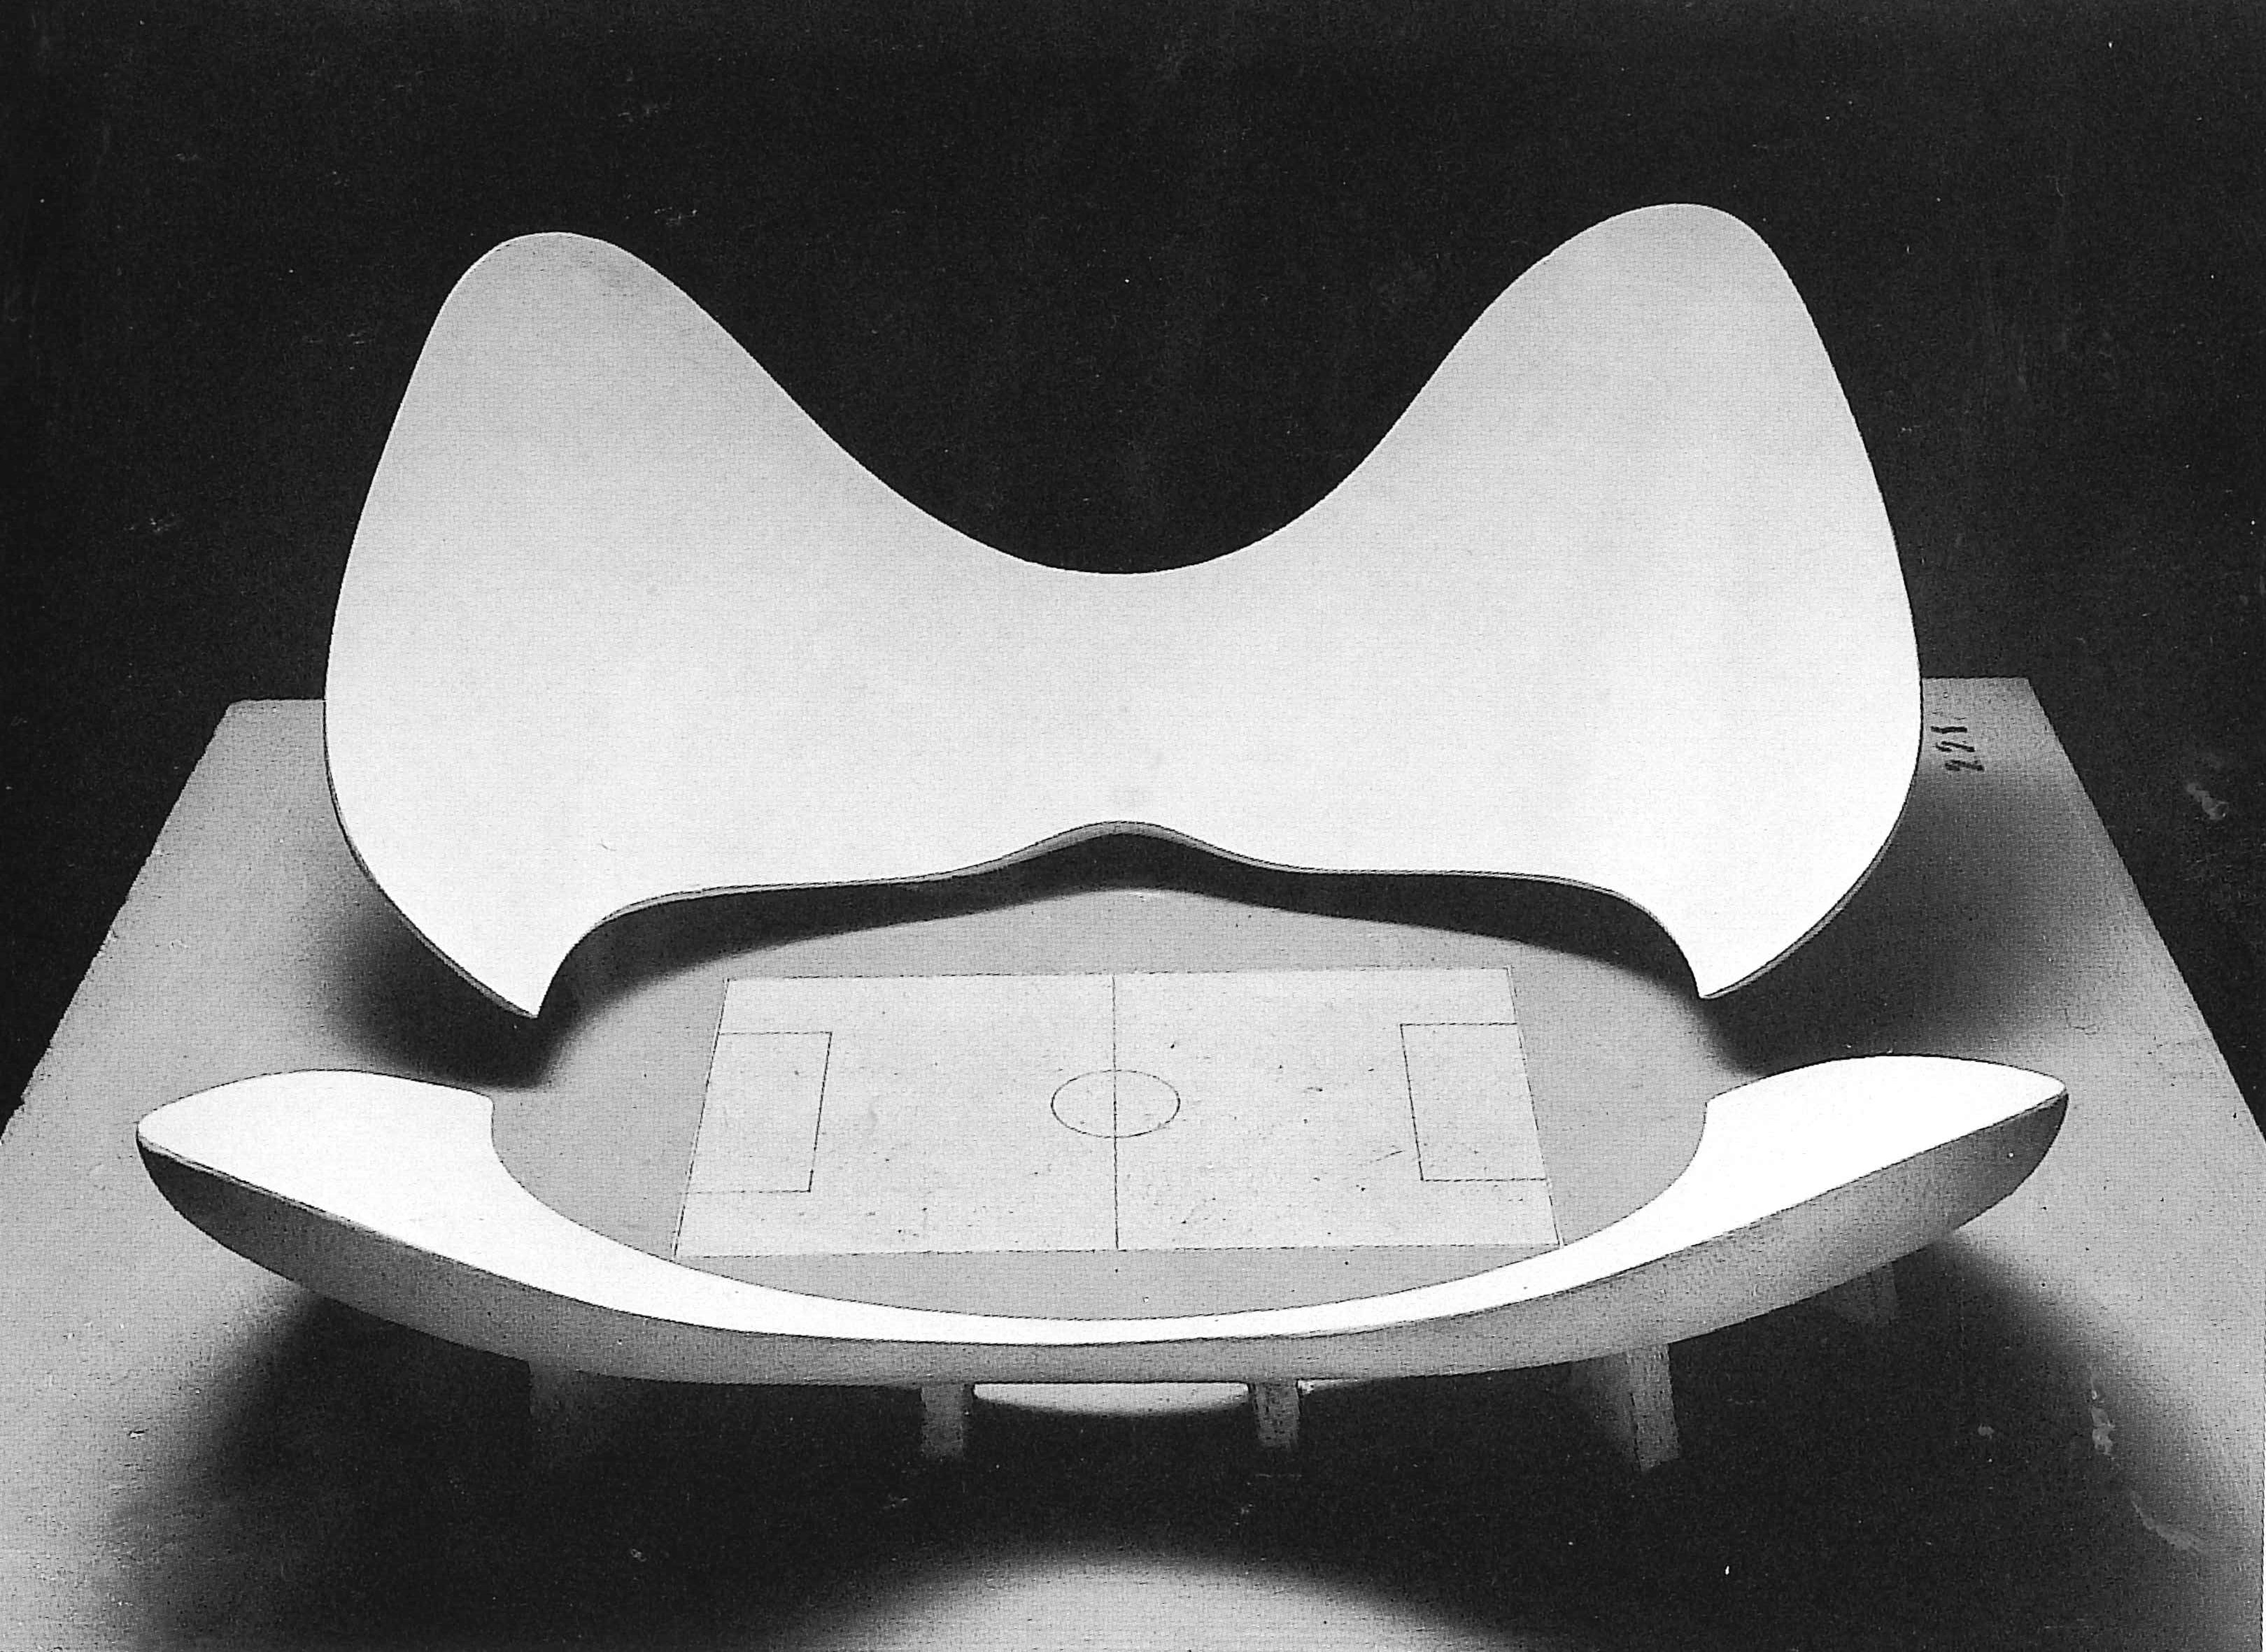
\includegraphics[width = \linewidth]{obrazky-figures/moretti_1.jpg}
    \caption{Model štadióna N od Luigi Moretti. Tento model bol vystavený na výstave parametrickej architektúry v~Twelfth Milan Triennial v~roku 1960. Parametrický model pozostávajúci z~devätnástich parametrov. Zdroj:  \cite{davis_2013}}
    \label{fig:morretiStadion}
\end{figure}

\begin{figure}[H]
    \centering
    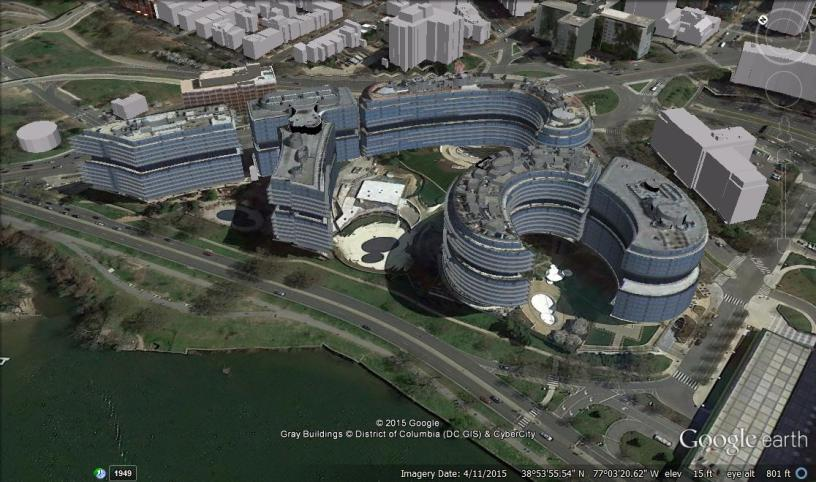
\includegraphics[width = \linewidth]{obrazky-figures/watergate-complex.jpg}
    \caption{Watergate Complex navrhnutý Luigi Morettim. Prvý veľký stavebný projekt, na ktorý boli využité parametrické modely. Zdroj: \cite{munger_2015}}
    \label{fig:Watergate}
\end{figure}





\section{Systémy pre tvorbu parametrických modelov} \label{sec:Existing_systems}
Existuje niekoľko systémov pre tvorbu parametrických modelov. Zväčša sú platené, ale sú aj také, ktoré umožňujú vytváranie modelov zdarma. Väčšinou tieto parametrické modelovacie systémy nie sú navrhnuté pre domáceho používateľa ale skôr pre profesionálnych 3D dizajnérov. Táto časť je podľa blogu \cite{gaget_2018}.


\subsection*{Solidworks}
Solidworks je jedným z~najlepších softvérov na tvorbu mechanických častí. Tento parametrický softvér je profesionálny nástroj pre inžinierov a dizajnérov. Umožňuje vykonať nad vytvoreným modelom aj rôzne simulácie, napríklad záťažové alebo tepelné ako je vidieť na obrázku \ref{fig:solidworks_simulations}.\nopagebreak
\begin{figure}[H]
    \centering
    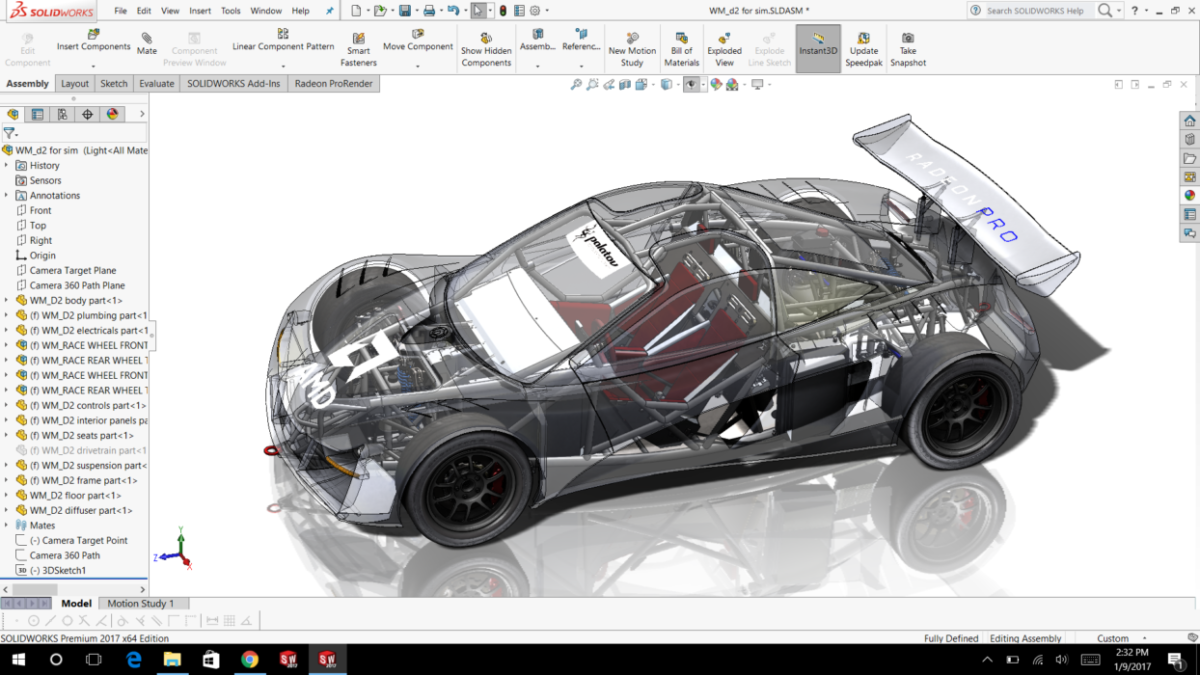
\includegraphics[width = 0.49\linewidth]{obrazky-figures/programs/solidworks_01.png}
    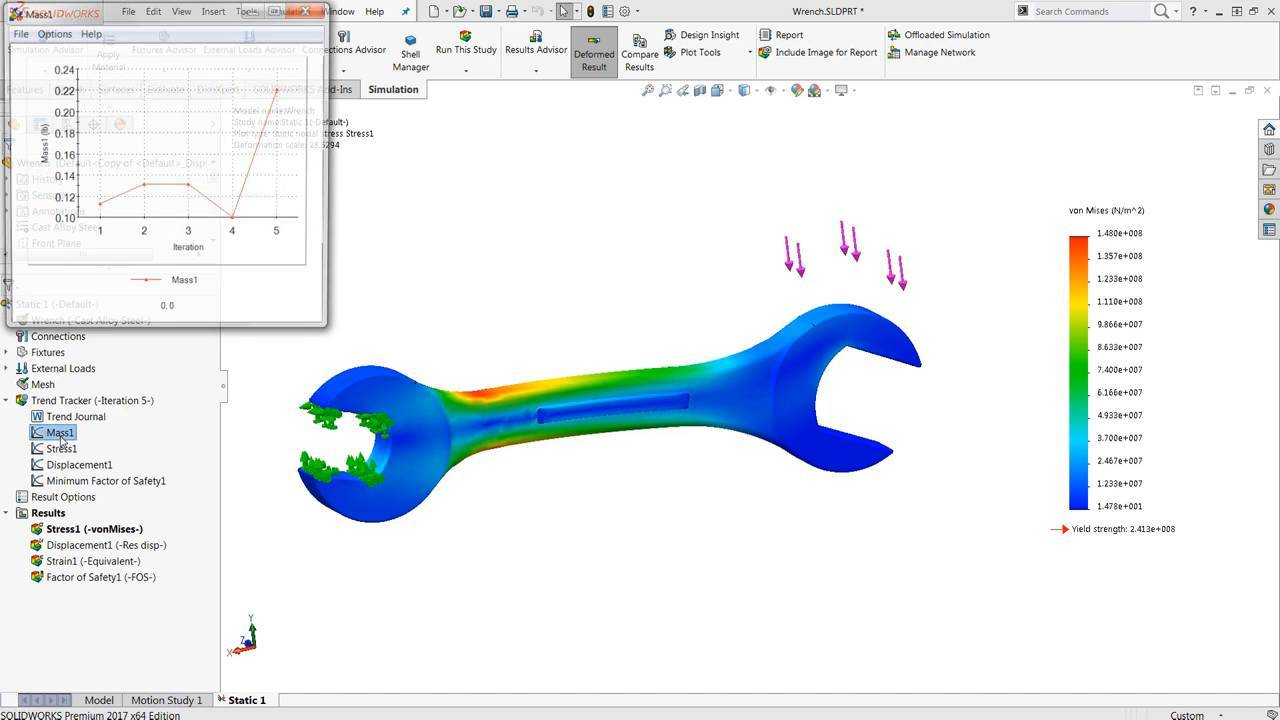
\includegraphics[width = 0.49\linewidth]{obrazky-figures/programs/solidworks, simulation.jpg}
    \caption{Prostredie programu Solidworks. Vpravo je záťažová simulácia. Zdroj: \cite{solidworks_2017} \cite{ames_2017} }
    % je tepelná simulácia \cite{goengineer_2014}
    \label{fig:solidworks_simulations}
\end{figure}


\subsection*{Catia}
Tento softvér je náročnejší pre menej zdatných užívateľov. Je to komplexný nástroj určený hlavne pre profesionálov a umožňuje množstvo pokročilejších nástrojov, ako je prevedenie dvojrozmerného obrázku do trojrozmerného modelu alebo generovanie organických tvarov, ktoré spĺňajú pevnostné požiadavky, ale sú od pôvodného modelu značne odľahčené \cite{technodat_cz_2017}.\nopagebreak
\begin{figure}[H]
    \centering
    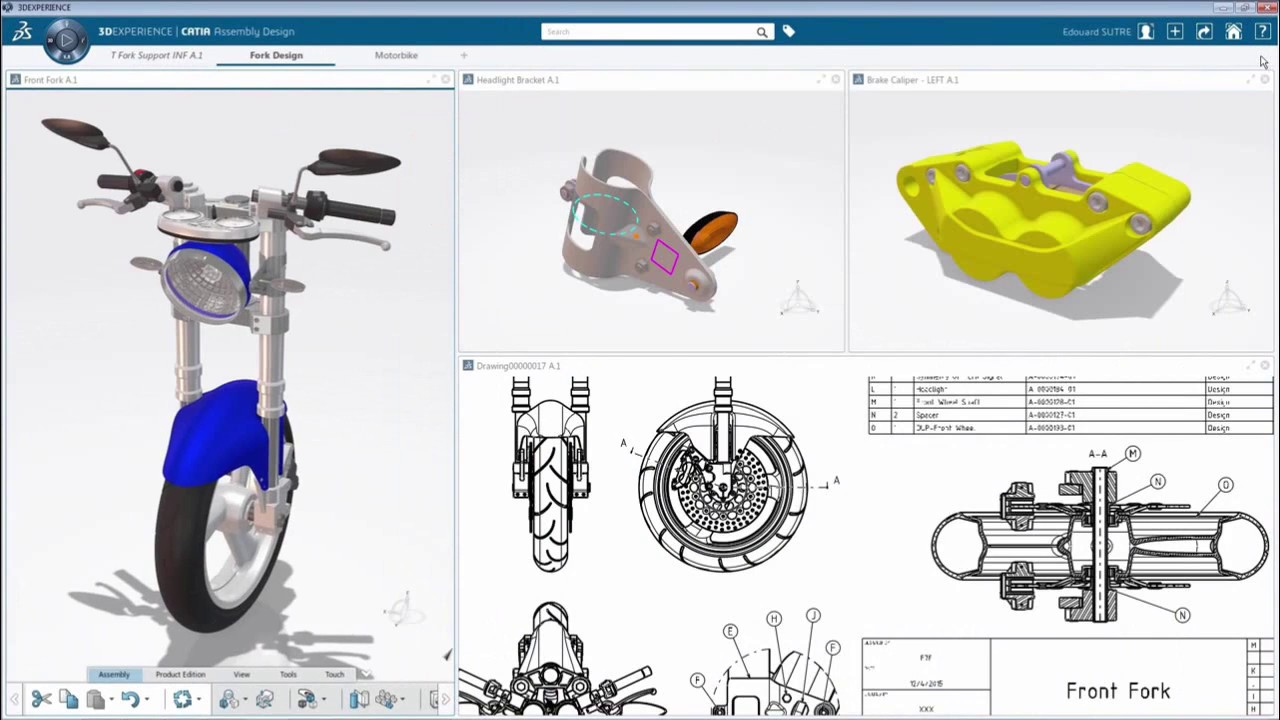
\includegraphics[width = 0.49\linewidth]{obrazky-figures/programs/Catia.jpg}
    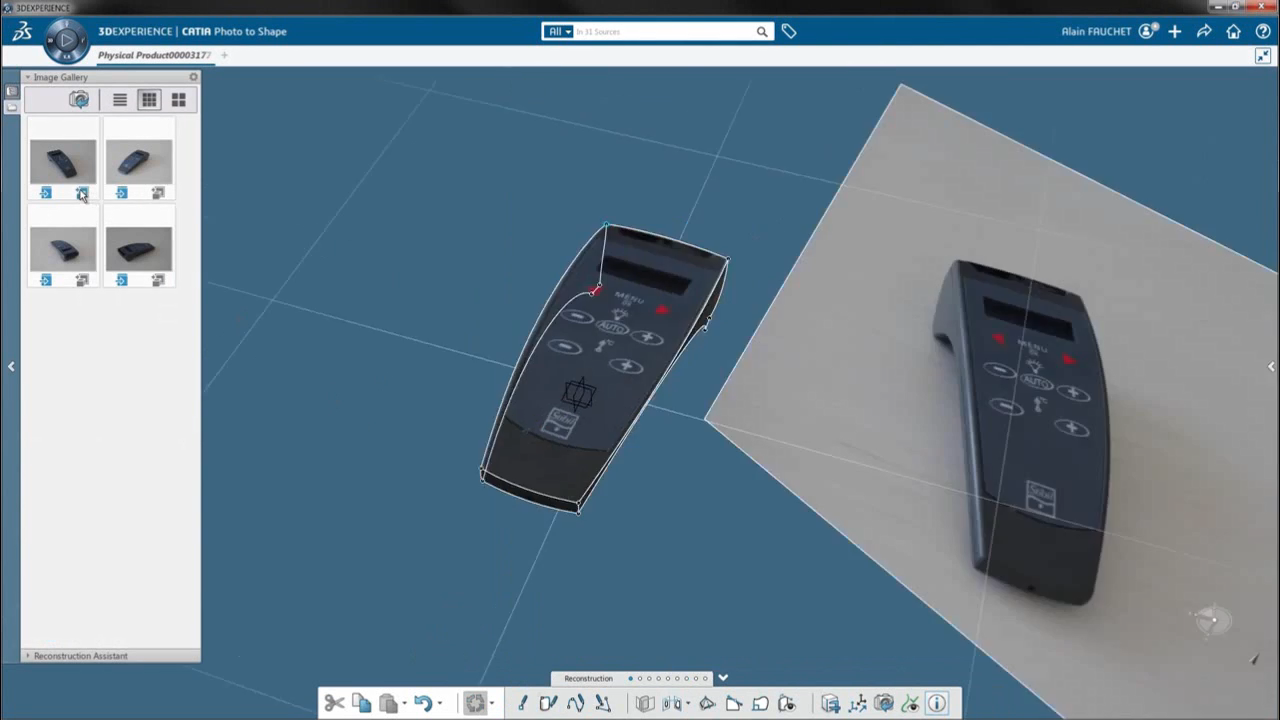
\includegraphics[width = 0.49\linewidth]{obrazky-figures/programs/Catia2.png}
    \caption{Prostredie programu Catia. Vpravo je ukážka prevodu z~2D obrázku do 3D modelu. Zdroj: \cite{technodat_cz_2017} }
    \label{fig:Catia}
\end{figure}


\subsection*{FreeCAD}
FreeCad je voľne dostupný softvér s~intuitívnym grafickým rozhraním. Umožňuje množstvo podobných nástrojov ako Catia a SolidWorks. Je zameraný na strojárstvo a návrh výrobku~\cite{freecad_2018}.\nopagebreak
\begin{figure}[H]
    \centering
    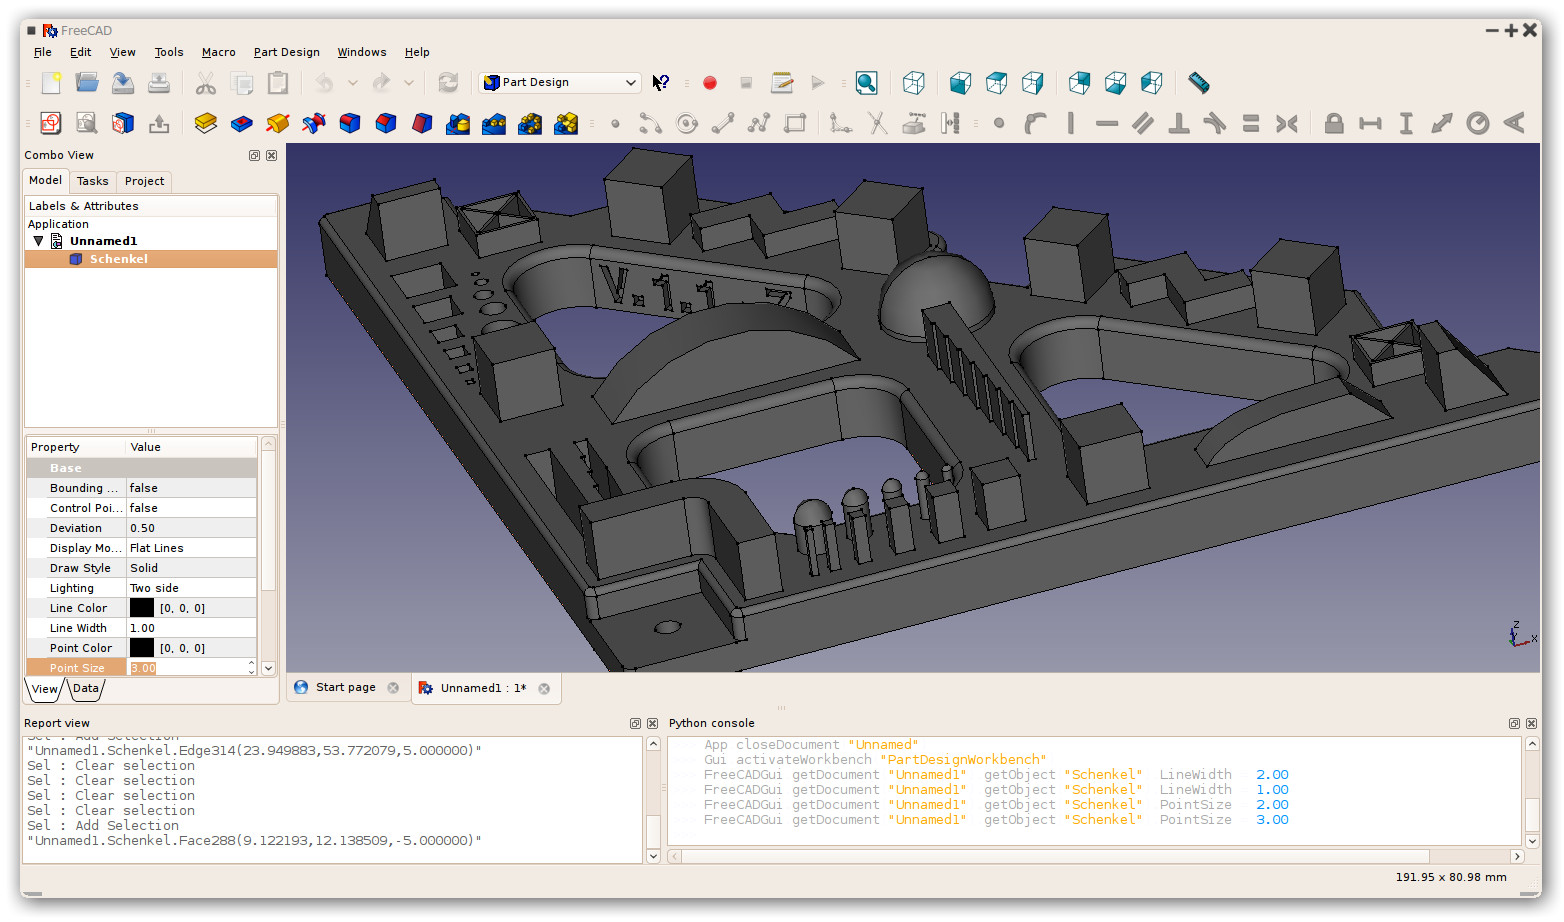
\includegraphics[width = 0.5\linewidth]{obrazky-figures/programs/Freecad_default.jpg}
    \caption{Prostredie programu FreeCAD. Zdroj: \cite{freecad_2018}}
    \label{fig:FreeCAD}
\end{figure}


\subsection*{Creo Parametric}
Jedná sa o~softvér pre priemyselný dizajn. Umožňuje vytvárať zložité trojrozmerné modely. Poskytuje veľa účinných nástrojov prispôsobených priemyselnému výrobnému prostrediu. Tento softvér sa často používa napríklad v~automobilovom priemysle.\nopagebreak
\begin{figure}[H]
    \centering
    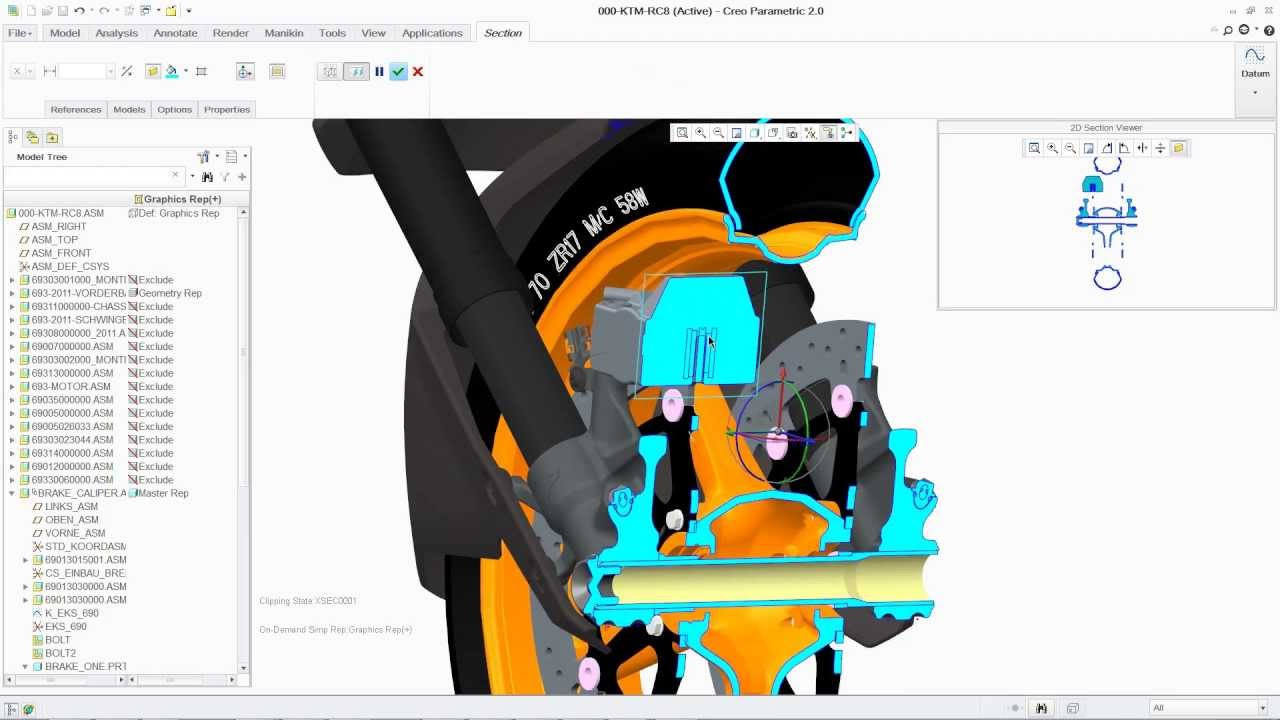
\includegraphics[width = 0.5\linewidth]{obrazky-figures/programs/Creo_Parametric.jpg}
    \caption{Prostredie programu Creo Parametric Zdroj: \cite{ptc_2013} }
    \label{fig:Creo}
\end{figure}


\subsection*{Rhino s~plugiom Grasshopper}
Rhino je profesionálny 3D CAD softvér používaný v~množstve spoločností. Pre prácu s~parametrickými modelmi je potrebný plugin Grasshopper. 

Grasshopper je vizuálny programovací jazyk, znázornený na obrázku \ref{fig:Grasshopper}.
Umožňuje tvorbu parametrických modelov pre konštrukčné inžinierstvo, architektúru a výrobu.\nopagebreak
\begin{figure}[H]
    \centering
    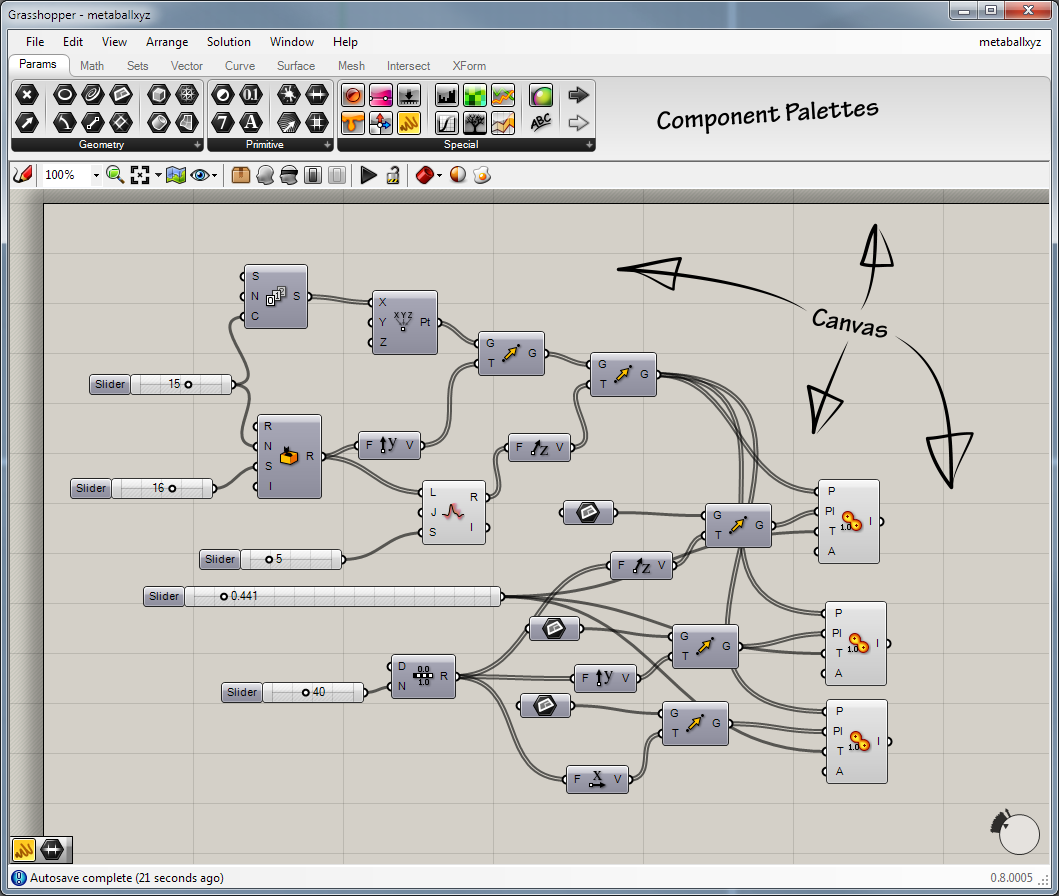
\includegraphics[width = 0.5\linewidth]{obrazky-figures/programs/Grasshopper_MainWindow.png}
    \caption{Prostredie programu Grasshopper Zdroj: \cite{rutten_2011} }
    \label{fig:Grasshopper}
\end{figure}


\subsection*{Fusion 360}
Fusion 360 nie je iba  parametrický modelovací systém. Podporuje aj priame modelovanie a umožňuje prechod medzi týmito typmi modelovania. Keďže pri priamom modelovaní nie je model vytváraný pomocou stromu operácií, je tento strom pri prenose odstránený. Má dobré simulačné a modelovacie nástroje, ktoré pomáhajú pri návrhu.\nopagebreak
\begin{figure}[H]
    \centering
    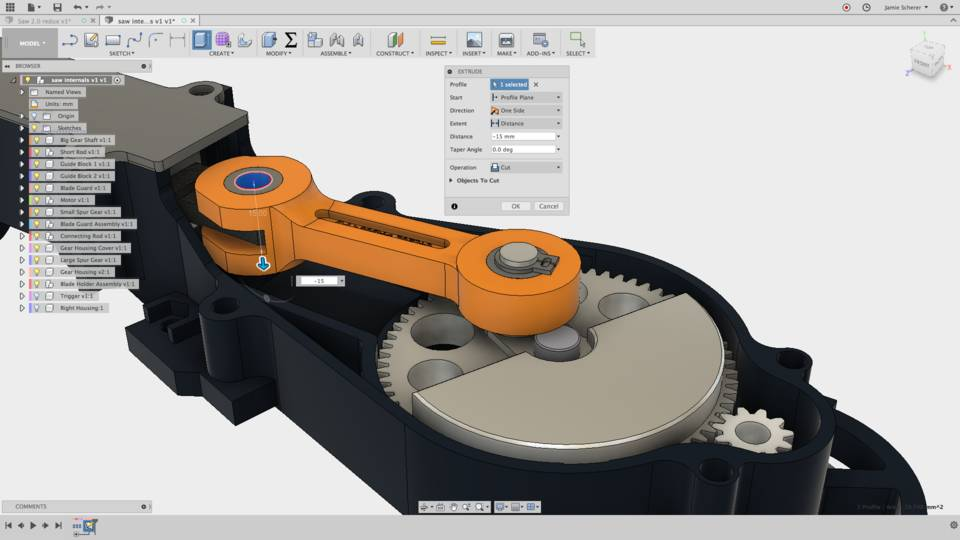
\includegraphics[width = 0.5\linewidth]{obrazky-figures/programs/Fusion.jpg}
    \caption{Fusion 360 Zdroj: \cite{gaget_2018} }
    \label{fig:Fusion}
\end{figure}

\subsection*{Inventor}
Inventor je rovnako ako Fusion 360 vytvorený spoločnosťou Autodesk. Tento program je často používaný v~strojárstve. Inventor ponúka množstvo parametrických možností, ktoré pomáhajú vytvárať 3D modely a hlavne mechanické konštrukcie.\nopagebreak
\begin{figure}[H]
    \centering
    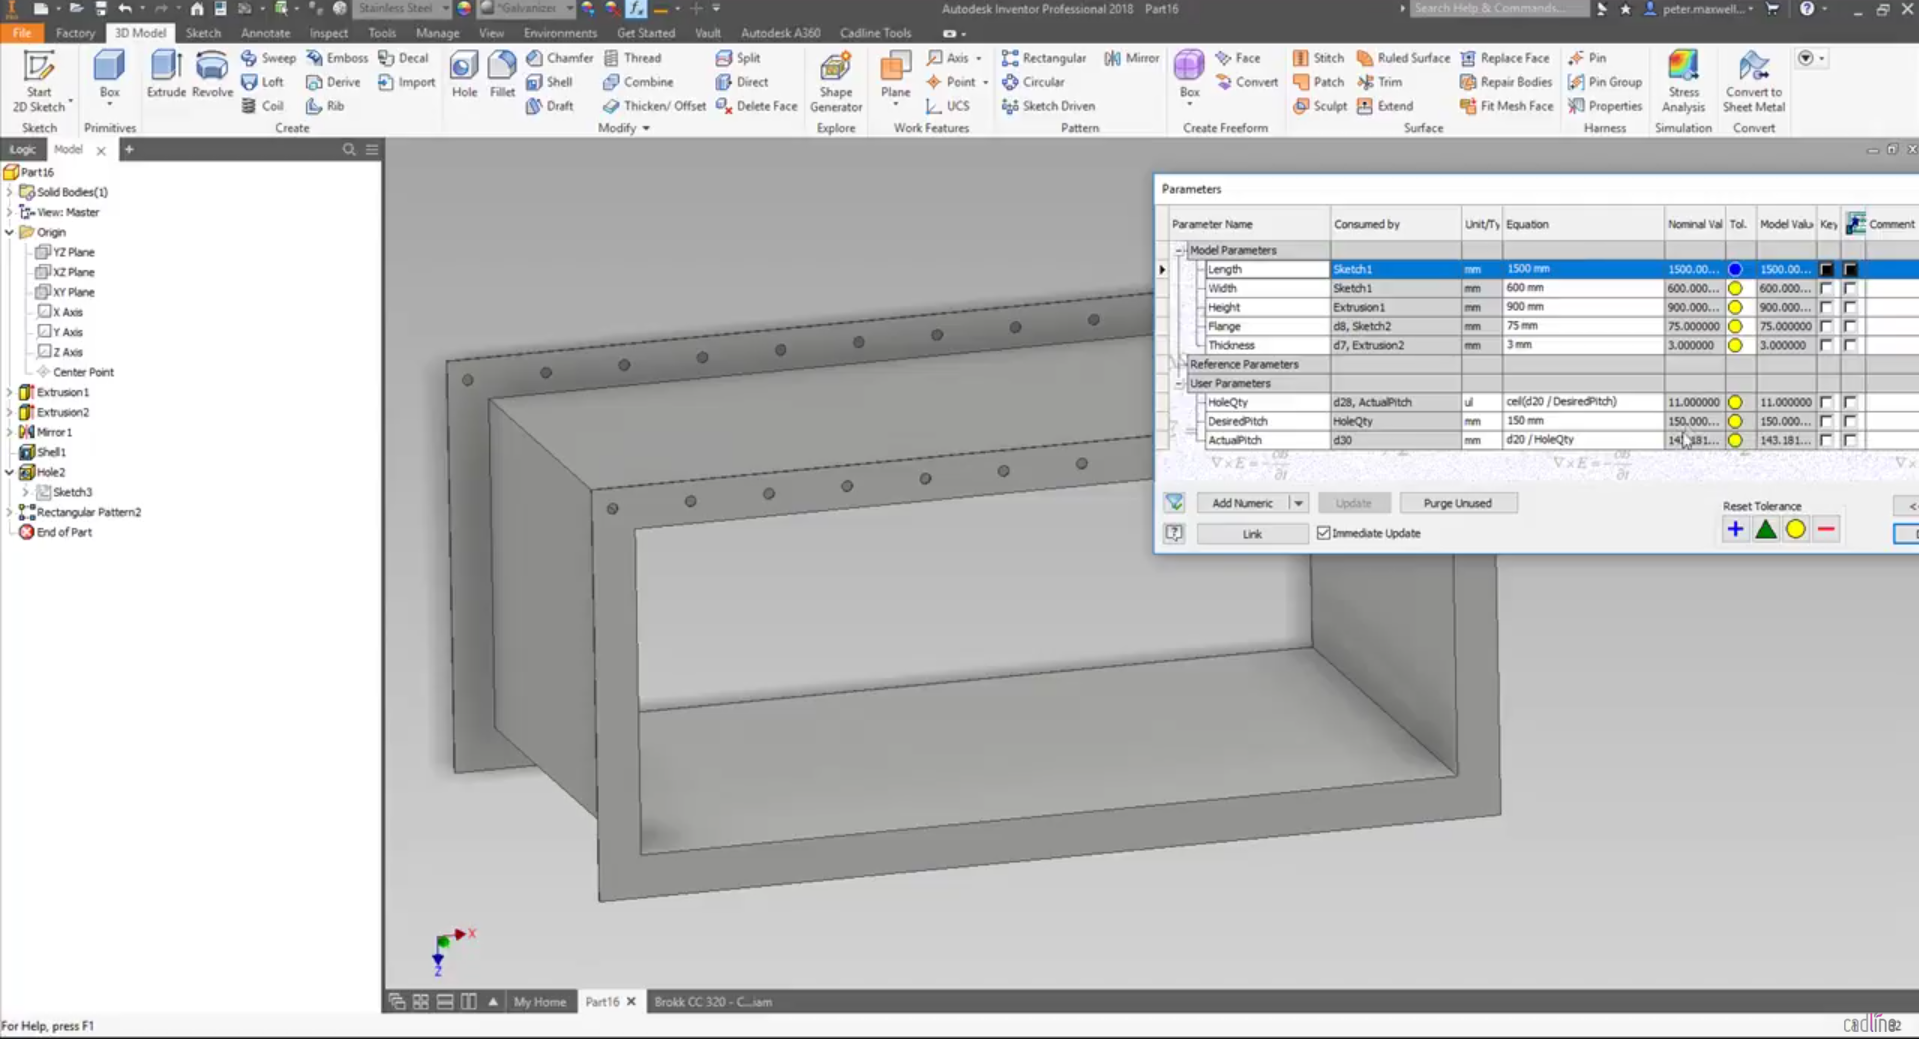
\includegraphics[width = 0.5\linewidth]{obrazky-figures/programs/Inventor.png}
    \caption{Inventor Zdroj: \cite{cadline_2017} }
    \label{fig:Inventor}
\end{figure}

\section{Existujúce knižnice na tvorbu trojrozmerných  modelov} \label{sec:existing_libraries}
Existuje niekoľko knižníc, ktoré umožňujú vytváranie trojrozmerných modelov. V tejto časti je opísaných niekoľko z nich.\nopagebreak
\subsection*{Libfive}
Libfive je knižnica  a sada nástrojov na modelovanie pevných látok, zvlášť vhodná na parametrické a procedurálne navrhovanie. Jazyk, ktorý knižnica používa na modelovanie objektov, je podobný jazyku Lisp.\nopagebreak
\begin{figure}[H]
    \centering
    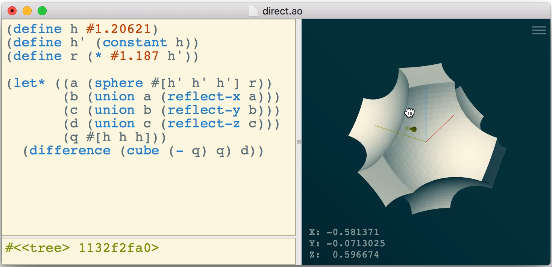
\includegraphics[width = 0.9\linewidth]{obrazky-figures/programs/libfive.png}
    \caption{Aplikácia Studio, používajúca knižnicu libfive. Zdroj: \cite{} }
    \label{fig:Inventor}
\end{figure}
\todo{cite https://libfive.com/studio/}

\subsection*{OpenSCAD}
\nopagebreak
\begin{figure}[H]
    \centering
    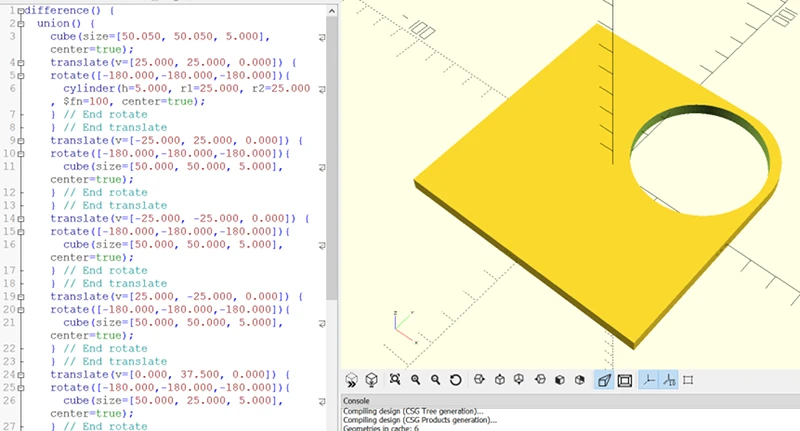
\includegraphics[width = 0.9\linewidth]{obrazky-figures/programs/openSCAD.png}
    \caption{Aplikácia Studio, používajúca knižnicu libfive. Zdroj: \cite{} }
    \label{fig:Inventor}
\end{figure}
\todo{cite https://www.openscad.org/documentation.html}


\subsection*{Tigl}
TiGL je knižnica, ktorá je určená hlavne pre geometrické modelovanie lietadiel a helikoptér. Je založená hlavne na vytváraní plôch pomocou kriviek NURBS.\nopagebreak
\begin{figure}[H]
    \centering
    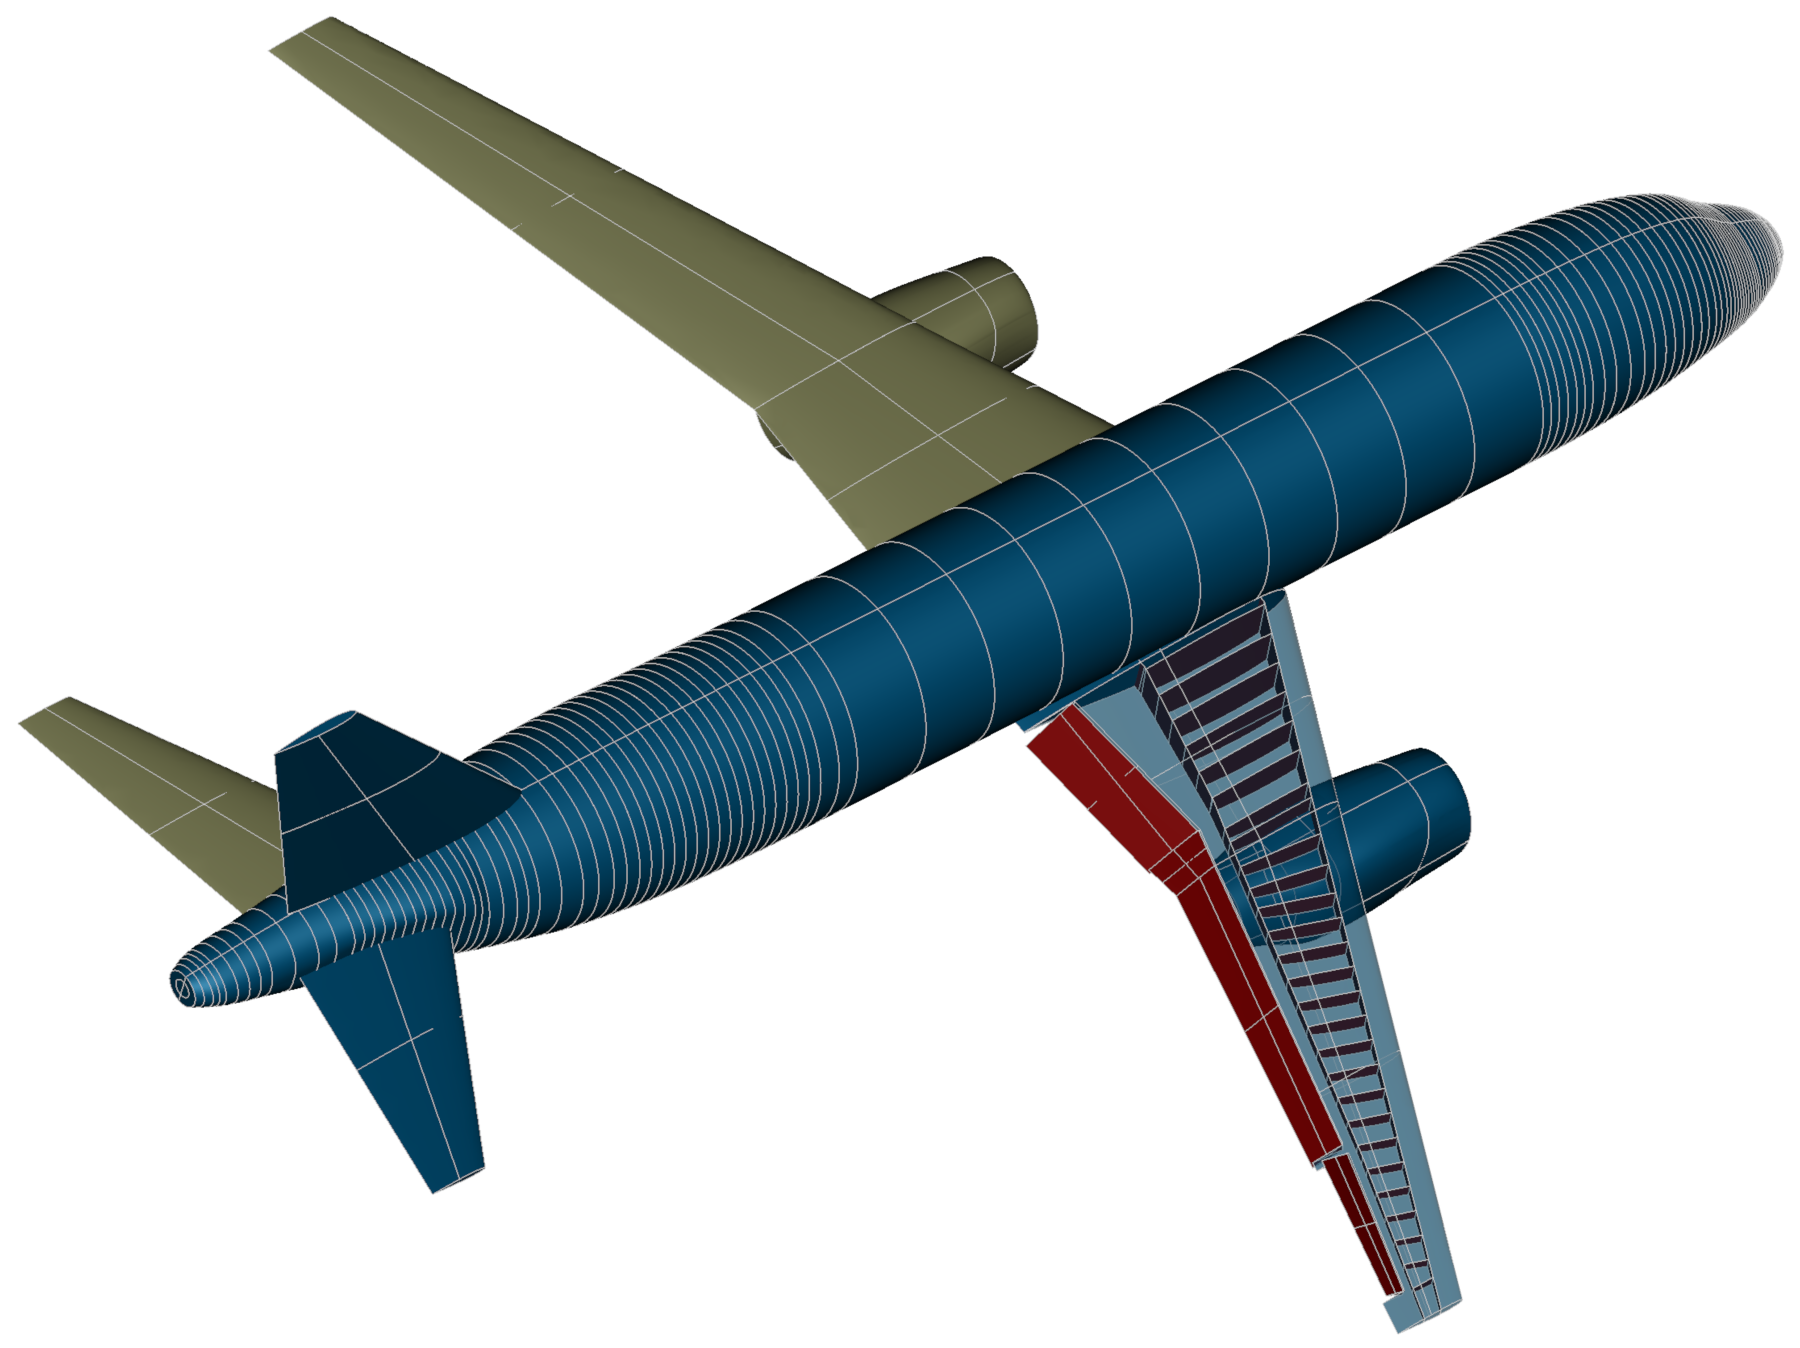
\includegraphics[width = 0.5\linewidth]{obrazky-figures/programs/tigl.png}
    \caption{Model vytvorený pomocou knižnice Tigl. Zdroj: \cite{} }
    \label{fig:Inventor}
\end{figure}
\todo{cite https://dlr-sc.github.io/tigl/pages/showcase.html}

\chapter{Geometrické objekty a operácie v~3D modelovaní}
\label{chapt:Geometrické_tvary}

Geometrické objekty môžeme rozdeliť do 4 kategórií podľa dimenzií. Body, úsečky, plochy a objemové objekty.
Spájaním objektov z~nižších dimenzií, vznikajú zložitejšie objekty z~vyšších dimenzií. 


Táto kapitola opisuje jednotlivé geometrické objekty a operácie, ktoré ich vytvárajú, a to od jednoduchších až k~zložitejším.

\section{Bod v 3D modelovaní}
Bod je základnou stavebnou jednotkou všetkých objektov. Všetky geometrické útvary sa dajú definovať ako množina bodov. Je to bezrozmerný geometrický útvar, teda nemá šírku, výšku ani hrúbku. Jeho úlohou je označiť pozíciu v~priestore. Pozíciu bodu v~trojrozmernom priestore udáva vzdialenosť na jednotlivých osiach ortogonálneho súradnicového systému X, Y a Z. Táto pozícia môže byť v~absolútnom tvare, teda od stredu súradnicového systému alebo v~relatívnom tvare, kedy je závislá na pozícii iného bodu.



\begin{figure}[H]
	\centering
	%\subfloat{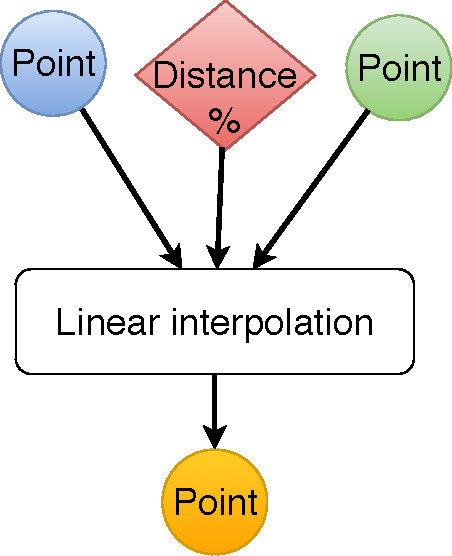
\includegraphics[height=0.3\textwidth]{obrazky-figures/Diagram/Point/DP Navrh operacii-0D - Point Linear interpolation.pdf}}
	\subfloat{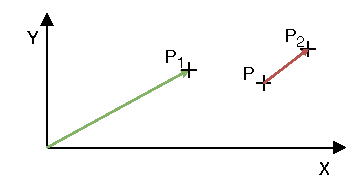
\includegraphics[height=0.3\textwidth]{obrazky-figures/Diagram/Draw/1Points/DP Navrh operacii-0D - Point.pdf}}
	\caption{Bod P$_1$ s~absolútnou pozíciou a bod P$_2$ s~relatívnou pozíciou od bodu P}
	\label{fig:Point}
\end{figure}

\subsection*{Lineárna interpolácia}
Lineárna interpolácia umožňuje získať bod, ktorý je na rovnakej priamke ako dva zadané body. Na obrázku \ref{fig:PointLinearInterpolation} sú tieto body zobrazené modrou a zelenou farbou, výsledný bod je zobrazený žltou farbou. Pozícia bodu závisí od zadanej vzdia\-le\-nos\-ti od počiatočného bodu. Táto vzdia\-le\-nosť môže byť zadaná dĺžkou alebo percentuálne, kde 50\% vytvorí bod uprostred počiatočného a koncového bodu. 




\begin{figure}[H]
	\centering
	%\subfloat{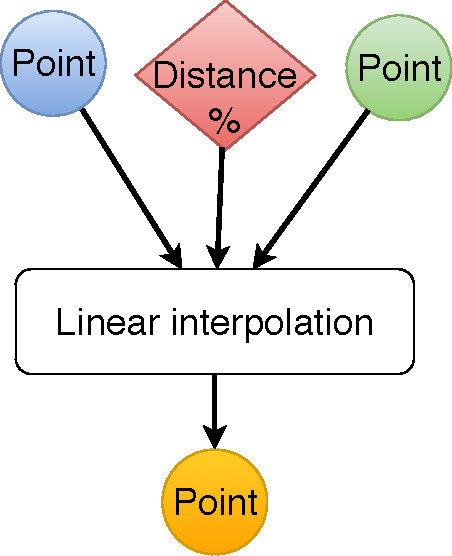
\includegraphics[height=0.3\textwidth]{obrazky-figures/Diagram/Point/DP Navrh operacii-0D - Point Linear interpolation.pdf}}
	\subfloat{
\includegraphics[height=0.3\textwidth]{obrazky-figures/Diagram/Draw/1Points/DP Navrh operacii-0D - PointLinearInterpolation.pdf}}
	\caption{Lineárna interpolácia medzi bodmi, kde \texttt{d} označuje vzdialenosť medzi zadanými bodmi a  \texttt{h} označuje vzdialenosť v~akej sa má vykonať interpolácia }
	\label{fig:PointLinearInterpolation}
\end{figure}

Ak je zadaná vzdialenosť pomocou dĺžky, použije sa vzorec \ref{eq:LiearnInterpolation}. Pri percentuálnej vzdialenosti sa použije obdobný vzorec, ale vektor medzi bodmi bod1 a bod2 sa nenormalizuje.
\begin{equation}
    bod = bod1 + norm(bod2 - bod1) * vzdialenos\check{t};
	\label{eq:LiearnInterpolation}
\end{equation}


\subsection*{Priesečník plochy a úsečky}

Pri tejto operácii sa používa ľubovolný plošný objekt ako rovina a úsečka ako priamka. Táto geometrická operácia vytvorí bod v~mieste, kde sa priamka pretína s~rovinou. 


\begin{figure}[H]
	\centering
	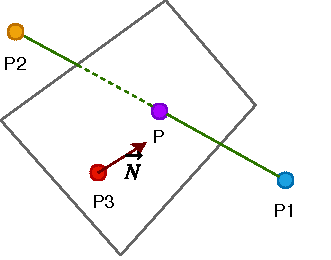
\includegraphics[height=0.3\textwidth]{obrazky-figures/DP Navrh operacii-Intersection.pdf}
	\caption{Pretnutie plochy priamkou}
	\label{fig:Intersection}
\end{figure}


Rovnica pre rovinu, ktorá je tvorená bodom \texttt{P\textsubscript{3}} nachádzajúcom sa na rovine a normálou N, sa dá zapísať ako \ref{eq:rovnicaPlochy_intersection} \cite{bourke_Point_Line_Plane}. 
\begin{equation}
    \textbf{N} \cdot (\textbf{P} - \textbf{P3}) = 0
	\label{eq:rovnicaPlochy_intersection}
\end{equation}
Rovnica priamky \ref{eq:rovnicaPriamky_intersection}, ktorá je určená bodmi \texttt{P\textsubscript{1}} a \texttt{P\textsubscript{2}}
\begin{equation}
	\textup{P}=\textbf{P1}+u (\textbf{P2}-\textbf{P1})
    \label{eq:rovnicaPriamky_intersection}
\end{equation}
Bod \texttt{P} označuje priesečník medzi rovinou a priamkou. Pomocou substitúcie získame rovnicu \ref{eq:rovnicaPriesecniku}.
\begin{equation}
	\textbf{N} \cdot (\textbf{P1}+u(\textbf{P2}-\textbf{P1}))) = \textbf{N} \cdot \textbf{P3}
    \label{eq:rovnicaPriesecniku}
\end{equation}
Po vyriešení tejto rovnice dostaneme rovnicu \ref{eq:rovnicaPriesecnikuSolved}. Výslednú pozíciu bodu dostaneme dosadením $u$ do rovnice pre  priamku \ref{eq:rovnicaPriamky_intersection}.
\begin{equation}
	u=\frac
{\textbf{N} \cdot (\textbf{P3}-\textbf{P1})}
{\textbf{N} \cdot (\textbf{P2}-\textbf{P1})}
    \label{eq:rovnicaPriesecnikuSolved}
\end{equation}


Ako je vidieť na obrázku \ref{fig:GraphIntersection_Plane_Line}, pomocou tejto operácie sa vytvorí bod aj mimo zadaných objektov. Problém nastáva, ak je zadaná úsečka paralelná s~plochou, a teda je kolmá na normálu plochy $N$. Skalárny súčin v~menovateli je potom rovný 0. V~tomto prípade priesečník buď neexistuje, alebo je priesečníkov nekonečne veľa, ak úsečka leží na rovine.

\begin{figure}[H]
	\centering
%	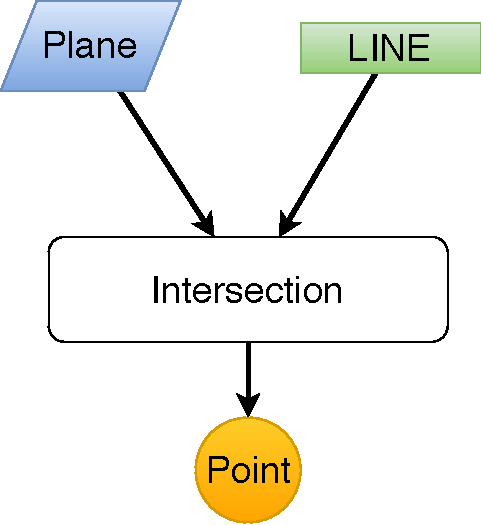
\includegraphics[height=0.3\textwidth]{obrazky-figures/Diagram/Point/DP Navrh operacii-0D - PointIntersection PlaneLine.pdf}
	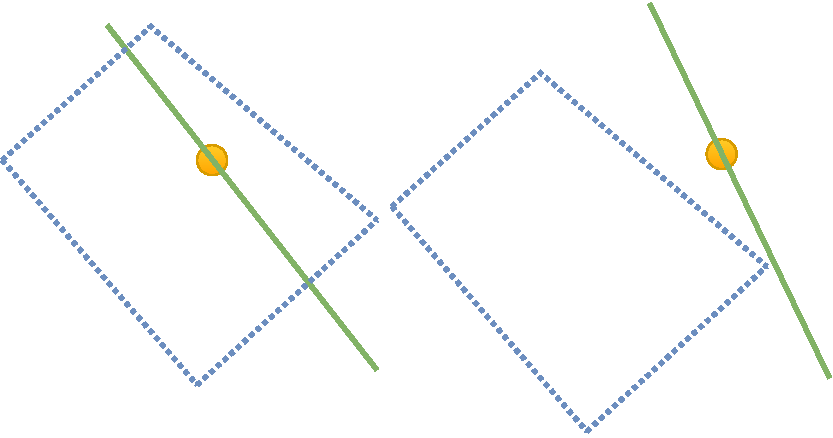
\includegraphics[height=0.3\textwidth]{obrazky-figures/Diagram/Draw/1Points/DP Navrh operacii-0D - PointIntersectionPlaneLine.pdf}
	\caption{Priesečník plochy a priamky. Vpravo je zobrazený prípad, ak sa priesečník nachádza na rovine, ale je mimo plochy objektu}
	\label{fig:GraphIntersection_Plane_Line}
\end{figure}

\subsection*{Stred plochy}
Existuje množstvo možností ako získať stred objektu. Do tejto práce som vybral dve metódy a to metódu minimálneho štvorca a priemer všetkých bodov. %Pri týchto operáciách sa prevádza zadaná plocha z trojrozmerného priestoru  do dvojrozmerného.


\subsubsection{Minimálny štvorec}
Pri tejto operácii sa prejdú všetky body a zistí sa maximálna a minimálna hodnota v~jednotlivých osiach. Výsledný bod sa nachádza uprostred nich.

%//Create point on position of middle of entered surface
%	//	Example:
%	//		SurfaceMiddle(PointName, Circle)	//- Create Point on center of Circle
%	//		SurfaceMiddle(PointName, Rectangle)	//- Create Point on middle of Rectangle
%	//		SurfaceCenter(PointName, Shape)		//- Create Point on middle of shape 
%	//		SurfaceMiddle(PointName, Shape)		//- Create Point on middle of shape - centroid (sum of points / count of points)

\begin{figure}[H]
	\centering
%	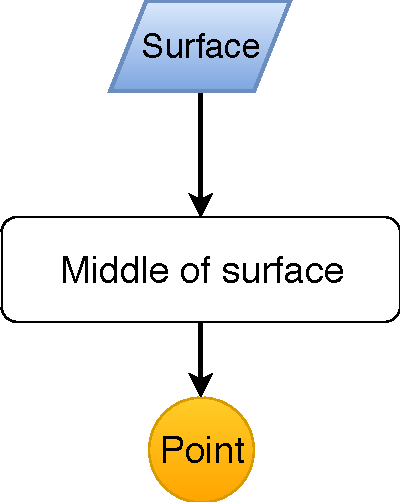
\includegraphics[height=0.3\textwidth]{obrazky-figures/Diagram/Point/DP Navrh operacii-0D - PointMiddle of surface.pdf}
	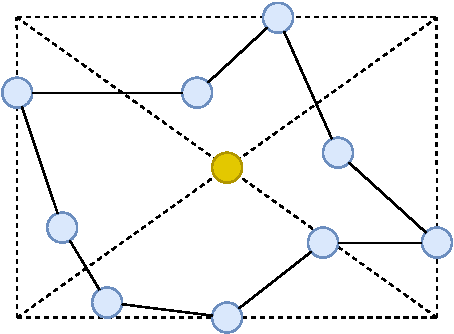
\includegraphics[height=0.3\textwidth]{obrazky-figures/Diagram/Draw/1Points/minimal square.pdf}
	\caption{Stred plochy pomocou minimálneho štvorca }
	\label{fig:PointMiddleofsurface}
\end{figure}



\subsubsection{Priemer všetkých bodov}
Nájdenie aritmetického priemeru všetkých bodov polygónu.

\begin{equation}
    \frac{1}{n} \sum_{i=0}^{n} p_i   
    \label{eq:aritPriemer}
\end{equation}


\subsubsection{Stred trojuholníka}
Aj pre trojuholník existuje množstvo typov stredu. V~súčastnosti je podľa encyklopédie stredov trojuholníkov známych až 30 714 trojuholníkových centier \cite{kimberling_2019}. Tento počet každým dňom narastá. Pre porovnanie, v~roku 1994 bolo známych 101, v~roku 1998 bolo 360 a v~decembri 2004 bolo známych 3053 \cite{Kimberling_Center_2004}. Medzi najznámejšie patria ťažisko (G), ortocentrum (H), stred vpísanej kružnice (I), opísanej kružnice (O) aj stred kružnice deviatich bodov (N). Tieto body sú zaznačené na obrázku \ref{fig:TriangleCenters}.


\begin{figure}[H]
	\centering
	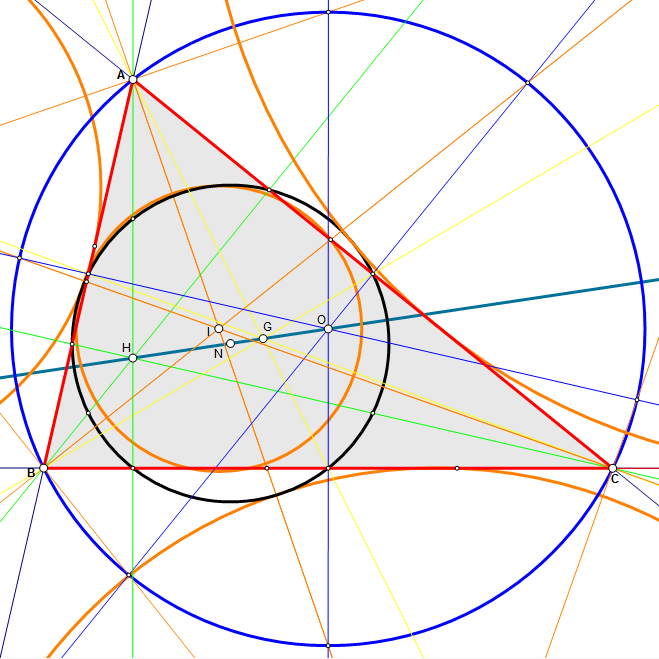
\includegraphics[width=0.9\textwidth]{obrazky-figures/Trigonometric_centres.png}
	\caption{Najznámejšie stredy trojuholníka sú ťažisko (G), ortocentrum (H), stred vpísanej kružnice (I), opísanej kružnice (O) aj stred kružnice deviatich bodov (N) \cite{triangle_center_2012}}
	\label{fig:TriangleCenters}
\end{figure}


 \mbox{} \\*
\paragraph{Ťažisko (angl. Centroid)}\unskip \mbox{} \\*

Ťažisko trojuholníka sa nachádza v~priesečníku troch mediánov trojuholníka. Na nájdenie jeho pozície stačí vypočítať aritmetický priemer vrcholov trojuholníka v~jednotlivých osiach \ref{eq:triangleCentroid} \cite{Centroid_of_a_Triangle}.



\begin{equation}
    \frac{A+B+C}{3}
    \label{eq:triangleCentroid}
\end{equation}

 \mbox{} \\*
\paragraph{Stred vpísanej kružnice (angl. Incenter)}\unskip \mbox{} \\*
\label{sec:TriangleCenter}

Z~každého bodu trojuholníka urobíme priamku tak, aby uhly na oboch stranách priam\-ky boli rovnaké. Táto priamka sa nazýva tiež bisektor \cite{angle_bisector_theorem}. Stred vpísanej kružnice je na priesečníku týchto priamok.




Stred vpísanej kružnice sa dá vypočítať aj pomocou vzorca \ref{eq:Incenter}, kde  $A$, $B$, $C$ sú vrcholy trojuholníka a $a$, $b$, $c$ sú dĺžky strán protiľahlých k~vrcholom $A$, $B$, $C$. \cite{Incenter_page_2011}.
\begin{equation}
O = \frac{a\ast A+b\ast  B +c \ast C}{a + b + c}
    \label{eq:Incenter}
\end{equation}


 \mbox{} \\*
\paragraph{Stred opísanej kružnice (angl. Circumcenter)}\unskip \mbox{} \\*

U~jednotlivých strán trojuholníka zistíme stred a z~tohto bodu urobíme kolmice. Tam kde sa tieto kolmice stretnú, vznikne stred vpísanej kružnice. Veľkosť kružnice je vzdialenosť od stredu k~ľubovoľnému vrcholu trojuholníka. Táto vzdialenosť je pre všetky vrcholy rovnaká.
 \mbox{} \\*

\paragraph{Ortocentrum (angl. Orthocenter)}\unskip \mbox{} \\*

Ortocentrum sa nachádza na priesečníku kolmíc, ktoré prechádzajú cez protiľahlý vrchol. Tieto kolmice sa tiež nazývajú výškou trojuholníka. 
Ak je trojuholník tupý, ortocentrum sa nachádza mimo trojuholníka, ak je trojuholník v~niektorom vrchole kolmý, nachádza sa v~takomto vrchole aj ortocentrum trojuholníka.

Pre získanie pozície ortocentra zistíme aspoň dve kolmice pomocou operácie \ref{sec:najkratsiauseckaBP}. Pozícia ortocentra sa nachádza v~mieste, kde sa tieto kolmice pretínajú. 


 \mbox{} \\*
\paragraph{Stred kružnice deviatich bodov (angl. NinePointCenter)}\unskip \mbox{} \\*

Kružnica deviatich bodov, tiež známa ako Feuefbachova kružnica, po nemeckom matematikovi Karl Wilhelm Feuerbach, ktorý ako prvý dokázal, že sa kružnica deviatich bodov dotýka vpísanej kružnice a pripísaných kružníc \cite{NinePointTheorem}.


\newtheorem{theorem}{Teorém}
 
\begin{theorem}[{\cite{vyznamne_prvky_trojuholnika} Teorém kružnice deviatich bodov}]
Nech ABC je všeobecný trojuholník, P,Q,R nech sú päty jeho výšok, K,L,M nech sú stredy jeho strán, O~nech je priesečník výšok a T,U,V nech sú postupne stredy úsečiek AO,BO,CO. Potom 9 bodov P, Q, R, K, L, M, T, U, V~leží na jednej (tzv. Feuerbachovej) kružnici. 

\end{theorem}


\begin{figure}[H]
	\centering
	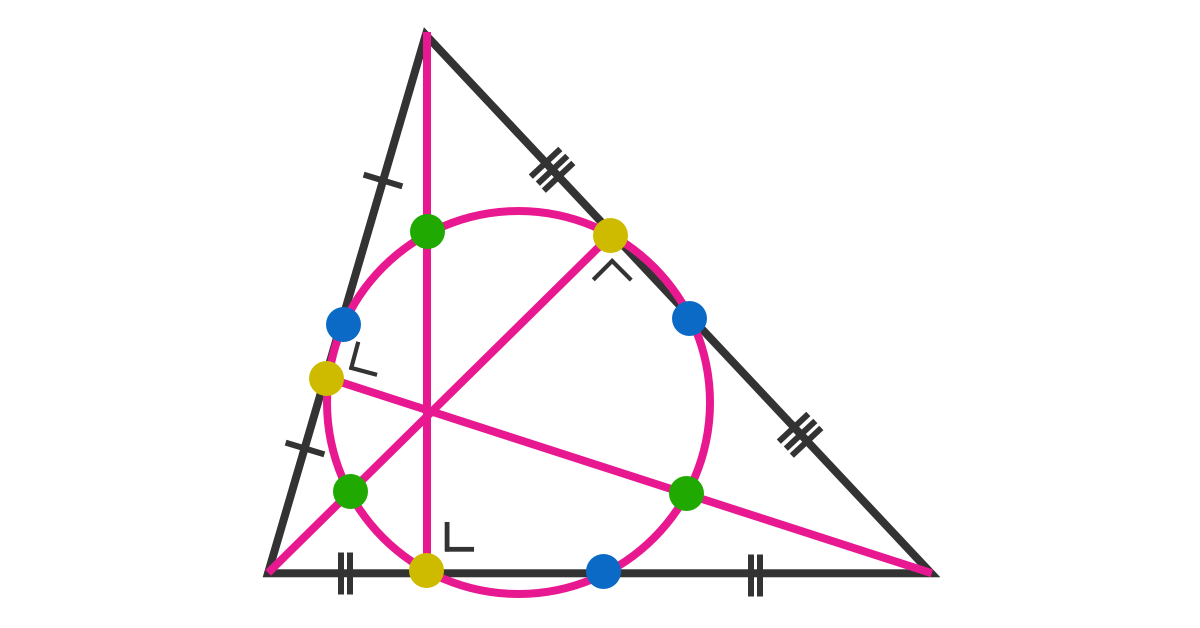
\includegraphics[width=0.9\textwidth]{obrazky-figures/NinePointCircle.png}
	\caption{Kružnica deviatich bodov. Modré body označujú stredy strán, žlté body označujú päty výšok a zelené sú stredy medzi vrcholmi a priesečníkom výšok\cite{katz_prakash_khim}}
	\label{fig:TriangleCenters_ninePoints}
\end{figure}



\subsection*{Stred objektu}
%https://www.gamedev.net/forums/topic/468405-center-of-a-3d-object/

Rovnako ako pri dvojrozmerných objektoch, je aj u~trojrozmerných objektoch viacero variánt získania stredu objektu. Zvolil som dve metódy, a to metódu ohraničujúceho kvádra a metódu priemerného stredu všetkých bodov.


\subsubsection{Stred pomocou ohraničujúceho kvádra}
Pri tejto metóde sa prejdú všetky body a zoberie sa maximálna a minimálna hodnota v~osiach X, Y a Z. Takto dostaneme ohraničujúci kváder (Bounding box) a ako výsledný bod sa zoberie stred tohto kvádra.
		
\begin{figure}[H]
	\centering
%	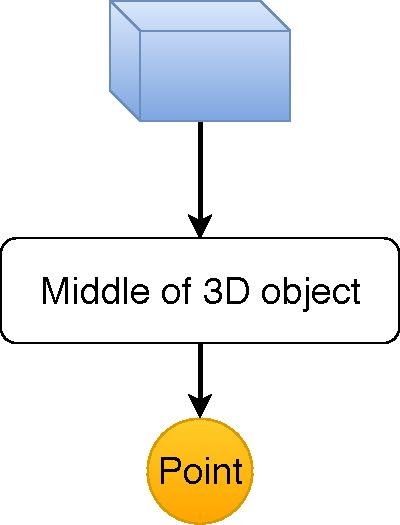
\includegraphics[height=0.3\textwidth]{obrazky-figures/Diagram/Point/DP Navrh operacii-0D - PointMiddle of 3D object.pdf}
	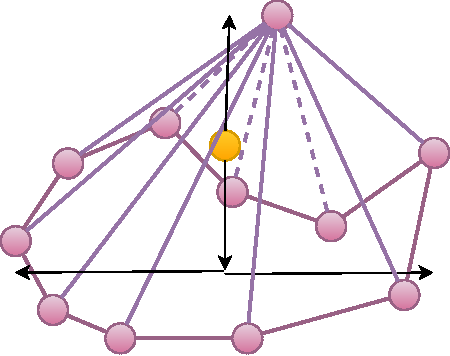
\includegraphics[height=0.3\textwidth]{obrazky-figures/Diagram/Draw/1Points/DP Navrh operacii-0D - PointMiddle of 3D object.pdf}
	\caption{Stred ohraničujúceho kvádra}
	\label{fig:PointMiddle of 3D object}
\end{figure}

\subsubsection{Ťažisko - Priemer všetkých bodov} 
Pri tejto operácii sa sčítajú koordináty všetkých bodov. To vytvorí tri veľké čísla, ktoré sa následne vydelia počtom bodov.


% \begin{figure}[H]
% 	\centering
% %	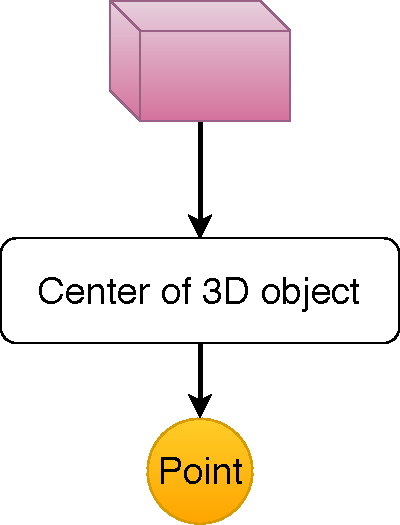
\includegraphics[height=0.3\textwidth]{obrazky-figures/Diagram/Point/DP Navrh operacii-0D - PointCenter of 3D object.pdf}
% 	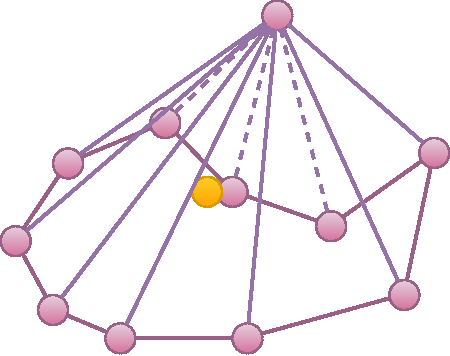
\includegraphics[height=0.3\textwidth]{obrazky-figures/Diagram/Draw/1Points/DP Navrh operacii-0D - PointCenter of 3D object.pdf}
% 	\caption{Priemerný všetkých bodov}
% 	\label{fig:1}
% \end{figure}








\section{Úsečky v 3D modelovaní}
Úsečka je časť priamky medzi dvoma koncovými bodmi. Aby bolo možné používať v~geometrických operáciách smerový vektor z~úsečky, môžeme tieto body označiť ako počiatočný a koncový, ako je zobrazené na obrázku \ref{fig:Navrh operacii-1D - Line}. 
%Úsečka sa nachádza v mnohých operáciach ako parameter, kde zastupuje úlohu smerového vektoru.

\begin{equation}
    P = P1 + u(P2-P1)
    \label{eq:priamka}
\end{equation}. 

\begin{figure}[H]
	\centering
%	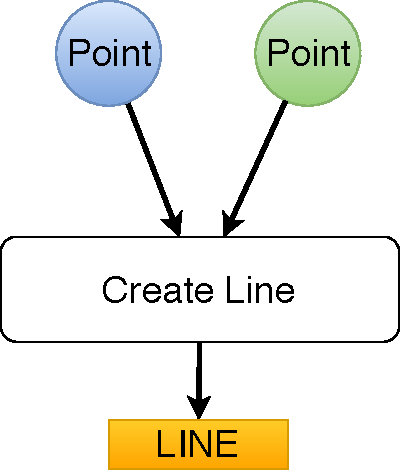
\includegraphics[height=0.3\textwidth]{obrazky-figures/Diagram/Line/DP Navrh operacii-1D - Line.pdf}
	
\includegraphics[]{obrazky-figures/Diagram/Draw/2Line/DP Navrh operacii-1D - Line.pdf}
	\caption{Zobrazenie úsečky s~počiatočným a koncovým bodom}
	\label{fig:Navrh operacii-1D - Line}
\end{figure}


\subsection*{Zmena dĺžky úsečky}
Vytvorenie úsečky so zadanou dĺžkou. Dĺžka môže byť zadaná vzdialenosťou alebo percentuálne od veľkosti zadanej úsečky. Výsledná úsečka je v~rovnakom smere a začína v~rovnakom bode ako zadaná úsečka. V~prípade, ak veľkosť výslednej úsečky sa rovná jedna, táto geometrická operácia sa nazýva aj normalizácia.  


\begin{figure}[H]
	\centering
%	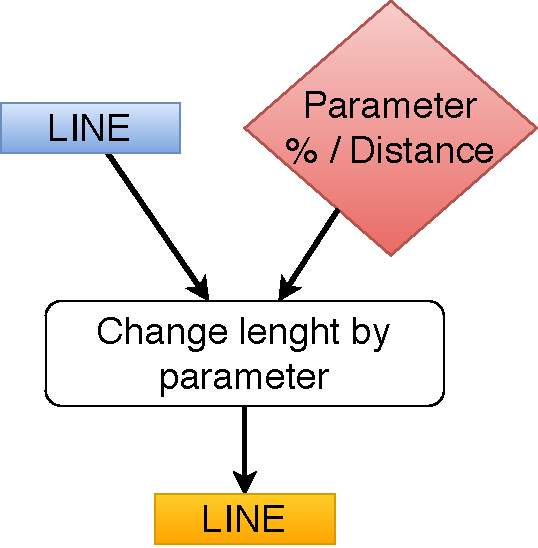
\includegraphics[height=0.3\textwidth]{obrazky-figures/Diagram/Line/DP Navrh operacii-1D - LineChangeLength.pdf}
	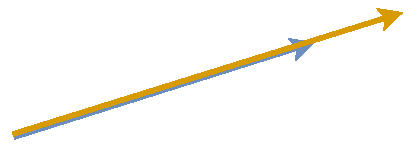
\includegraphics[]{obrazky-figures/Diagram/Draw/2Line/DP Navrh operacii-1D - LineChangeLength.pdf}
	\caption{Zmena veľkosti úsečky}
	\label{fig:LineChangeLength}
\end{figure}

\subsection*{Najkratšia úsečka medzi bodom a priamkou}\label{sec:najkratsiauseckaBP}
Priamka je definovaná dvoma bodmi, bodom $P1(x1-y1)$ a bodom $P2(x2,y2)$. 
Rovnica priamky je \ref{eq:MinlinePointLine_LineEq}.
\begin{equation}
    P = P1 + u(P2-P1)
    \label{eq:MinlinePointLine_LineEq}
\end{equation}

Na získanie najkratšej vzdialenosti je potrebné nájsť kolmicu od bodu $P3(x3,y3)$ na priamku. Z~toho vyplýva, že skalárny súčin medzi nimi musí byť rovný 0, tento vzťah je vidieť v~rovnici \ref{eq:MinlinePointLine_LinesEq}.

\begin{equation}
    (P3-P)\cdot(P2-P1) =0 
    \label{eq:MinlinePointLine_LinesEq}
\end{equation}
Bod P označuje najbližší bod na priamke k~bodu $P3$.

Substitúciou rovnice \ref{eq:MinlinePointLine_LineEq} do \ref{eq:MinlinePointLine_LinesEq} získame rovnicu \ref{eq:MinlinePointLine_subs}.

\begin{equation}
[P3 - P1 - u(P2-P1)] \cdot (P2 - P1) = 0
    \label{eq:MinlinePointLine_subs}
\end{equation}

Vyriešením tejto rovnice získame rovnicu \ref{eq:MinlinePointLine_subsSolved}, ktorú následne môžeme dosadiť do rovnice pre priamku \ref{eq:MinlinePointLine_LineEq} a získať pozíciu bodu $P$. Ak by sme chceli, aby sa bod vytváral iba na úsečke a nie mimo nej, bolo by potrebné testovať vzdialenosť $u$, či je v rozmedzí (0,1). Ak je hodnota $u$ záporná alebo väčšia ako jedna,  najbližší bod na priamke k~bodu $P3$ sa nachádza mimo zadanej úsečky. 
\begin{equation}
u= \frac
{\left (x3 -x1  \right )\left (x2-x1  \right )
+\left (y3-y1  \right )\left (y2-y1  \right )
+\left (z3-z1  \right )\left (z2-z1  \right )}
{\left \| P2-P1 \right \|^{2}}
    \label{eq:MinlinePointLine_subsSolved}
\end{equation}
Výsledná úsečka je tvorená bodmi $P$ a $P3$ \cite{bourke_Point_Line_Plane}.
%Pre získanie bodu na priamke, ktorý je najbližšie k bodu $P3$ je možné následne použiť operáciu pre získanie počiatočného bodu úsečky .



\begin{figure}[H]
	\centering
%	\includegraphics[height=0.3\textwidth]{obrazky-figures/Diagram/Line/DP Navrh operacii-1D -  LineMinPL.pdf}
	\includegraphics[height=0.3\textwidth]{obrazky-figures/Diagram/Draw/2Line/DP Navrh operacii-1D -  LineMinPL.pdf}
	\caption{Najkratšia vzdialenosť medzi úsečkou a bodom}
	\label{fig:LineMinPL}
\end{figure}

\subsection*{Najkratšia úsečka medzi dvomi priamkami}
Keďže v~trojrozmernom priestore často nenastáva pretnutie dvoch úsečiek v~jednom bode, je práve najkratšia úsečka medzi dvoma priamkami používaná ako priesečník priamok v~trojrozmernom priestore.


Hľadáme najkratšiu úsečku s~bodmi $P_a$ a $P_b$, kde $P_a$ leží na priamke definovanou bodmi $P_1$ a $P_2$, a $P_b$ leží na priamke, ktorá je definovaná bodmi $P_3$ a $P_4$.

Pre bod $P_a$ môžeme napísať rovnicu  \ref{eq:MinlineLL_Pa}.
\begin{equation}
P_a=P_1 + u_a(P_2-P_1)
    \label{eq:MinlineLL_Pa}
\end{equation}
Podobne pre bod $P_b$ rovnicu \ref{eq:MinlineLL_Pb}.
\begin{equation}
P_b=P_3 + u_b(P_4-P_3)
    \label{eq:MinlineLL_Pb}
\end{equation}
Pri hľadaní najkratšej úsečky medzi týmito priamkami si stačí uvedomiť, že najkratšia úsečka bude na tieto priamky kolmá, čo nám umožňuje zapísať následovné rovnice  \ref{eq:MinlineLL_dotab}.
\begin{equation}
\begin{aligned}
(P_a-P_b) \cdot (P_2-P_1) =0\\
(P_a-P_b) \cdot (P_4-P_3) =0
\end{aligned}
    \label{eq:MinlineLL_dotab}
\end{equation}
Po doplnení  $P_a$ a $P_b$ do týchto rovníc získame rovnice \ref{eq:MinlineLL_dotabExp}.
\begin{equation}
\begin{aligned}
((P_1 + u_a(P_2-P_1))-(P_3 + u_b(P_4-P_3))) \cdot (P_2-P_1) =0\\
((P_1 + u_a(P_2-P_1))-(P_3 + u_b(P_4-P_3))) \cdot (P_4-P_3) =0
\end{aligned}
    \label{eq:MinlineLL_dotabExp}
\end{equation}
Keďže by tieto rovnice boli veľmi rozsiahle, je vhodné si pre riešenie tejto rovnice definovať nasledovnú substitúciu \ref{eq:MinlineLL_subsdmnop}.
\begin{equation}
d_{mnop}=(x_m - x_n)(x_o-x_p)+(y_m - y_n)(y_o-y_p)+(z_m - z_n)(z_o-z_p)
    \label{eq:MinlineLL_subsdmnop}
\end{equation}
Pomocou tejto substitúcie sa dajú rovnice \ref{eq:MinlineLL_dotabExp} zapísať nasledovne \ref{eq:MinlineLL_dotabExpshort}.
\begin{equation}
\begin{aligned}
d_{1321} + u_a d_{2121} - u_b d_{4321} = 0\\
d_{1343} + u_a d_{2143} - u_b d_{4343} = 0
\end{aligned}
    \label{eq:MinlineLL_dotabExpshort}
\end{equation}
Vyriešením týchto rovníc pre $u_a$ získame rovnicu \ref{eq:MinlineLL_dotabExpshortSolving}.
\begin{equation}
 u_a= \frac
 {d_{1343} d_{4321} - d_{1321} d_{4343} }
 {d_{2121} d_{4343} - d_{2143} d_{2143} }
    \label{eq:MinlineLL_dotabExpshortSolving}
\end{equation}
Keď už poznáme $u_a$, pomocou dosadenia do rovnice \ref{eq:MinlineLL_dotabExpshortSolved_ub} získame $u_b$ \cite{bourke_Point_Line_Plane}.
\begin{equation}
\begin{aligned}
u_b  = \frac{d_{1321} + u_a d_{2121}}{d_{4321}}
\end{aligned}
    \label{eq:MinlineLL_dotabExpshortSolved_ub}
\end{equation}



\begin{figure}[H]
	\centering
%	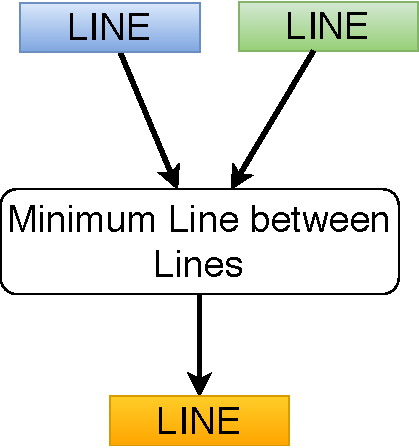
\includegraphics[height=0.3\textwidth]{obrazky-figures/Diagram/Line/DP Navrh operacii-1D - LineMinLL.pdf}
	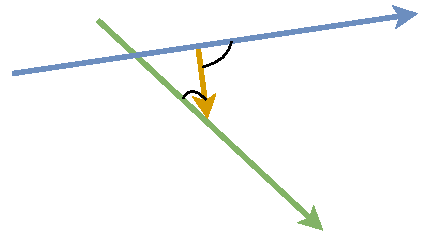
\includegraphics[height=0.3\textwidth]{obrazky-figures/Diagram/Draw/2Line/DP Navrh operacii-1D - LineMinLL.pdf}
	\caption{Najkratšia vzdialenosť medzi dvomi úsečkami}
	\label{fig:LineMinLL}
\end{figure}


\subsection*{Najkratšia úsečka medzi plochou a bodom}


Rovina je definovaná pomocou normály $\overrightarrow{N}=(A, B, C)$ a bodom na nej ležiacom $P_a=(x_a,y_a,z_a)$.
Hľadaná úsečka má rovnaký smer ako normála plochy.
Vzdialenosť medzi touto rovinou a bodom $P_b=(x_b,y_b,z_b)$ dostaneme pomocou vzorca \ref{eq:minlineSP}, kde premietneme vektor medzi bodom $P_b$ a bodom $P_a$ na normálu roviny $\overrightarrow{N}$ pomocou skalárneho súčinu. 
\begin{equation}
 distance = (P_b - P_a) \cdot \overrightarrow{N}
    \label{eq:minlineSP}
\end{equation}

Bod $P$ získame vynásobením vektora $\overrightarrow{N}$ touto vzdialenosťou a následným odčítaním od bodu $P_b$ \ref{eq:minlineSP_P}.
\begin{equation}
 P = P_b - (\overrightarrow{N} * distance)
    \label{eq:minlineSP_P}
\end{equation}

Výsledná úsečka má počiatočný bod na ploche a koncový bod $P_b$ \cite{bourke_Point_Line_Plane}.

%Každý bod $P=(x,y,z)$ leží na rovine, ak splňuje \ref{eq:rovnicaPlochySP}.
%\begin{equation}
%Ax+By+Cz+D = 0
%    \label{eq:rovnicaPlochySP}
%\end{equation}




\begin{figure}[H]
	\centering
%	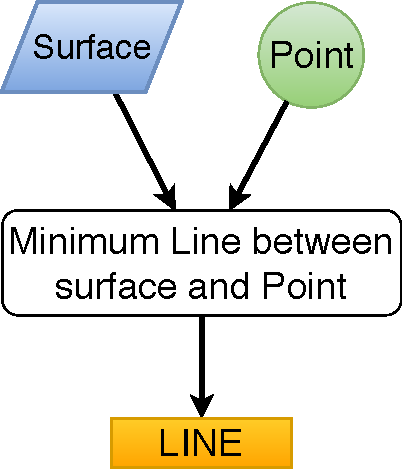
\includegraphics[height=0.3\textwidth]{obrazky-figures/Diagram/Line/DP Navrh operacii-1D - LineMinSP.pdf}
	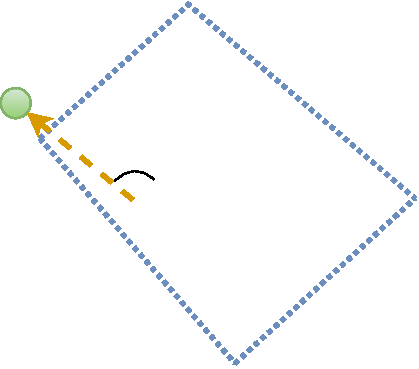
\includegraphics[height=0.3\textwidth]{obrazky-figures/Diagram/Draw/2Line/DP Navrh operacii-1D - LineMinSP.pdf}
	\caption{Najkratšia vzdialenosť medzi plochou a bodom}
	\label{fig:LineMinSP}
\end{figure}


\subsection*{Vektorový súčin}\label{subsec:crossproduct}
Vektorový súčin (cross product) vytvára úsečku, ktorá je kolmá na dané úsečky (priamky). Zadané úsečky sa najprv prevedú na vektory ($koncov\acute{y}\_bod - za\check{c}iato\check{c}n\acute{y}\_bod$).
Veľkosť úsečky závisí od veľkosti zadaných úsečiek a od uhla, ktorý zvierajú. 

\begin{equation}
 L_1 \times L_2 =  \{
 y_{l1} z_{l2} + y_{l2} z_{l1} ,
 z_{l1} x_{l2} + z_{l2} x_{l1} ,
 x_{l1} y_{l2} + x_{l2} y_{l1}\}
    \label{eq:cross}
\end{equation}


\begin{figure}[H]
	\centering
%	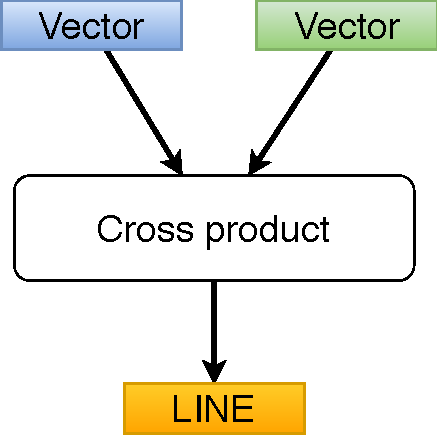
\includegraphics[height=0.3\textwidth]{obrazky-figures/Diagram/Line/DP Navrh operacii-1D - LineCross.pdf}
	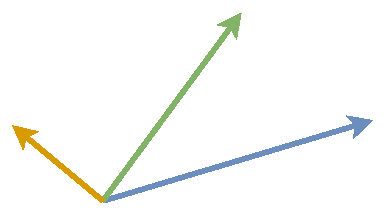
\includegraphics[height=0.3\textwidth]{obrazky-figures/Diagram/Draw/2Line/DP Navrh operacii-1D - LineCross.pdf}
	\caption{Vektorový súčin}
	\label{fig:LineCross}
\end{figure}

Táto operácia sa často používa aj v~počítačovej grafike, kde sa používa pre výpočet normály plošných útvarov. Výsledný vektor sa musí normalizovať, teda vydeliť jeho dĺžkou.
% \subsection*{Normála roviny}
% Normála plochy sa pri väčšine plošných objektov predvypočítava už pri vytváraní. Ak objekt nebol vytváraný už priamo so zadanou normálou, je potrebné ju vypočítať. Výpočet normály sa robí pomocou vektorového súčinu \ref{subsec:crossproduct}, ktorého výsledný vektor je potrebné normalizovať, teda vydeliť jeho dĺžkou.



% \subsection*{Presun úsečky}
% Táto operácia nepremiestňuje zadanú úsečku ale vytvára úsečku v rovnakom smere a rovnakej dĺžke ako zadaná úsečka $L$, ale počiatočný bod bude na pozícii zadaného bodu $P$. 
% Koncový bod úsečky $P2$ získame pomocou vzorca \ref{eq:LineReloc}. 

% \begin{equation}
%     P2 = P + (P_{2L}-P_{1L})
%     \label{eq:LineReloc}
% \end{equation}




% \begin{figure}[H]
% 	\centering
% %	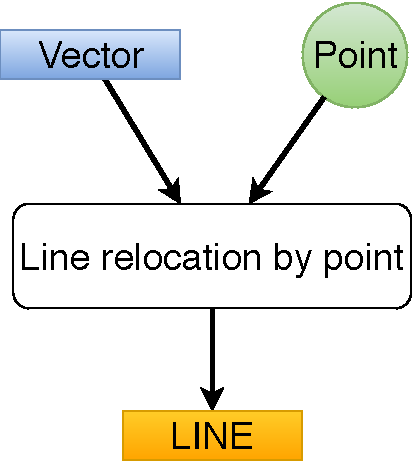
\includegraphics[height=0.3\textwidth]{obrazky-figures/Diagram/Line/DP Navrh operacii-1D - LineRelocation.pdf}
% 	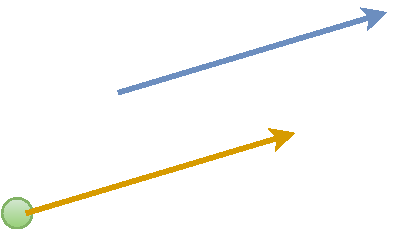
\includegraphics[height=0.3\textwidth]{obrazky-figures/Diagram/Draw/2Line/DP Navrh operacii-1D - LineRelocation.pdf}
% 	\caption{Presun úsečky}
% 	\label{fig:1}
% \end{figure}

\section{Plošné objekty v 3D modelovaní}


\subsection*{Kruh}
Je viac metód ako zadávať kruh. Základným spôsobom pre vytvorenie kruhu je zadanie stredového bodu a priemeru. Keďže chceme aby bol kruh v~trojrozmernom priestore, je potrebné zadať aj normálu. 

Ďalším spôsobom je zadanie troch bodov, kde jeden z~bodov označuje stred kruhu, druhý bod leží na obvode kruhu a tretí bod ležiaci na ploche kruhu tak, aby nebol s~ostatnými bodmi na jednej priamke, označuje natočenie kruhu.

\begin{figure}[H]
	\centering
	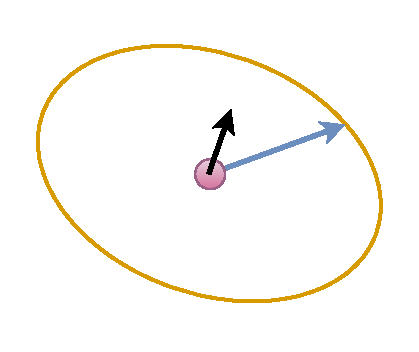
\includegraphics[height=0.3\textwidth]{obrazky-figures/Diagram/Draw/3Plane/DP Navrh operacii-2D - SurfaceCreate Circle.pdf}
	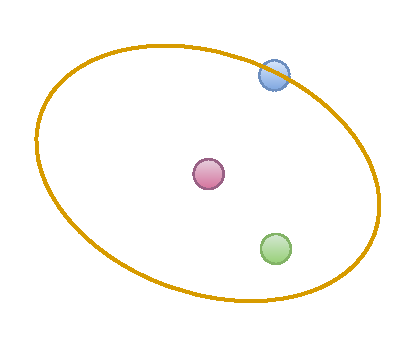
\includegraphics[height=0.3\textwidth]{obrazky-figures/Diagram/Draw/3Plane/DP Navrh operacii-2D - SurfaceCreate Circle2.pdf}
	\caption{Vľavo je kruh pomocou priemeru a normály a v~pravo je kruh tvorený troma bodmi, kde jeden bod udáva stred a pomocou ďalších dvoch bodov sa určí priemer a smer normály}
	\label{fig:SurfaceCreate Circle2}
\end{figure}

Alternatívne môžeme vyjadriť kruh pomocou opísanej (Circumscribed) alebo vpísanej (Inscribed) kružnice trojuholníka (obrázok \ref{fig:SurfaceInscribed Circumscribed Circle}). Postup pre nájdenie stredu opísanej a vpísanej kružnice trojuholníka je v~časti \ref{sec:TriangleCenter}.



\begin{figure}[H]
	\centering
	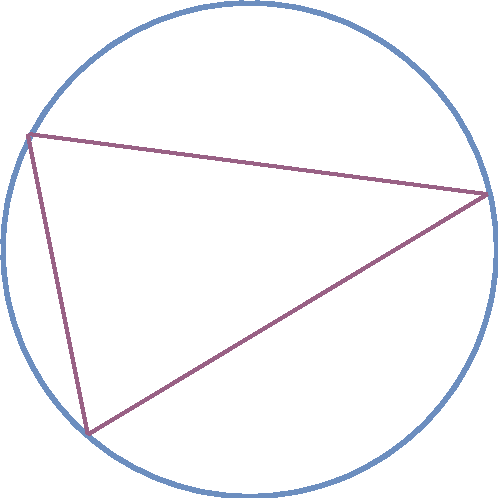
\includegraphics[height=0.3\textwidth]{obrazky-figures/Diagram/Draw/3Plane/DP Navrh operacii-2D - SurfaceCircumscribed Circle.pdf}
	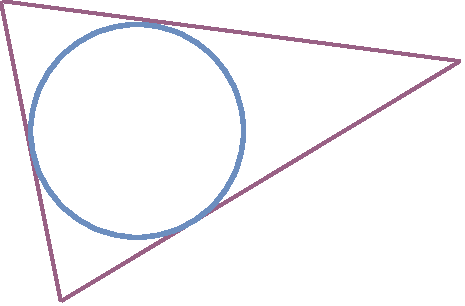
\includegraphics[height=0.3\textwidth]{obrazky-figures/Diagram/Draw/3Plane/DP Navrh operacii-2D - SurfaceInscribed Circle.pdf}
	\caption{Opísaná a vpísaná kružnica trojuholníka}
	\label{fig:SurfaceInscribed Circumscribed Circle}
\end{figure}



\subsection*{Obdĺžnik}
Často používaným geometrickým objektom v~modelovaní je aj obdĺžnik. Základnými parametrami obdĺžnikov je výška a šírka. Ďalším parametrom je často aj natočenie okolo normály. Keďže sa zaoberáme objektami v~trojrozmernom priestore, obdĺžnik musí definovať aj normála, ako je vidieť na obrázku \ref{fig:SurfaceCreate Rectangle}. 


\begin{figure}[H]
	\centering

	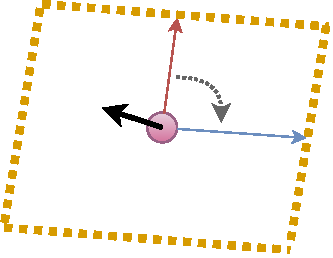
\includegraphics[height=0.3\textwidth]{obrazky-figures/Diagram/Draw/3Plane/DP Navrh operacii-2D - SurfaceCreate Rectangle.pdf}
	\caption{Obdĺžnik}
	\label{fig:SurfaceCreate Rectangle}
\end{figure}



\subsection*{Polygón}
Keďže v~reálnom svete nie sú základom objektov len dokonalé objekty ako kruh, trojuholník alebo štvorec, zvolil som pre túto prácu aj tvorbu polygónov. Polygóny pozostávajú z~množiny bodov a množinou hrán, ktoré tieto body spájajú a vytvárajú obvod polygónu. Keďže polygón je plošný útvar, musí byť tvorený minimálne 3 bodmi. Táto operácia má ako jediná premenlivý počet bodov. 

Všetky primitívne objekty, ako štvorec, kruh alebo trojuholník, sú konvexné, teda všetky vnútorné uhly sú menšie alebo rovné 90 stupňov. Proces triangulácie je v~tomto prípade veľmi jednoduchý. Stačí spojiť jeden ľubovoľný bod so všetkými ostatnými bodmi. Pri zadávaní polygónov pomocou bodov sa ale môže stať, že niektorý vnútorný uhol polygónu bude tupý, teda väčší ako 90 stupňov. Klasická metóda triangulácie teda nepostačuje a je potrebné vybrať niektorú inú metódu, napríklad \textit{Ear clipping method}.















































\section{Objemové objekty v 3D modelovaní}
Medzi základné geometrické objemové telesá patrí guľa, kváder, valec, a ihlan. Nad týmito geometrickými telesami je možné vykonávať rôzne geometrické operácie.


% \subsection{Valec}


% \begin{figure}[H]
% 	\centering
% 	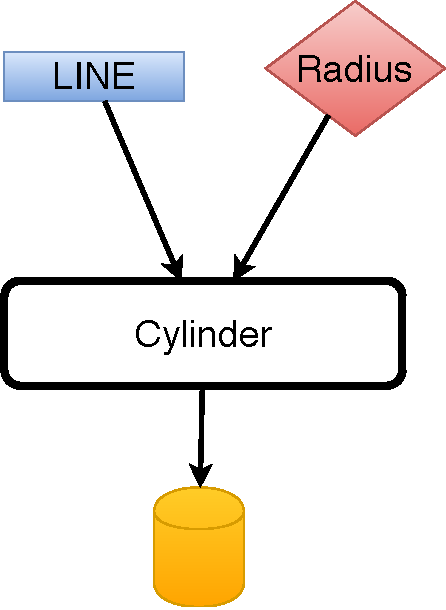
\includegraphics[height=0.3\textwidth]{obrazky-figures/Diagram/Volumetric/DP Navrh operacii-3D - ObjectsCylinder.pdf}
% 	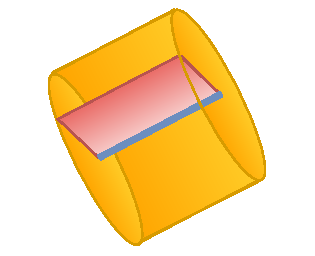
\includegraphics[height=0.3\textwidth]{obrazky-figures/Diagram/Draw/4Object/DP Navrh operacii-3D - ObjectsCylinder.pdf}
% 	\caption{Valec}
% 	\label{fig:ObjectsCylinder}
% \end{figure}

% \subsection*{Guľa}


% \subsection*{Ihlan}


\begin{figure}[H]
	\centering
% 	\includegraphics[height=0.3\textwidth]{obrazky-figures/Diagram/Draw/4Object/DP Navrh operacii-3D - ObjectsCreate Pyramid by distance from center.pdf}
	\includegraphics[height=0.3\textwidth]{obrazky-figures/Diagram/Draw/4Object/DP Navrh operacii-3D - ObjectsCreate Pyramid.pdf}
	\caption{Ihlany s~rôznymi základmi.}
	\label{fig:ObjectsCreate Pyramid}
\end{figure}


\subsection*{Extrudovanie} 
Natiahne plochu do priestoru v~smere normály, čím získa na objeme. Pomocou tejto operácie sa dá vytvoriť aj napríklad kváder alebo valec, ak je základ štvorcového, respektívne kruhového tvaru. Táto operácia je zobrazená na obrázku \ref{fig:ObjectsExtrude}, kde je fialovým zobrazená počiatočná plocha a žltým je zobrazená extrudácia. Extrudáciu je možné spraviť tak, že sa vytvorí kópia zadanej plochy a posunie sa o~zadaný offset. Tieto dve plochy sa následne prepoja. Častou modifikáciou je extrudovanie po krivke a/alebo postupná zmena veľkosti. 




\begin{figure}[H]
	\centering
% 	\includegraphics[height=0.3\textwidth]{obrazky-figures/Diagram/Volumetric/DP Navrh operacii-3D - ObjectsExtrude.pdf}
	\includegraphics[height=0.3\textwidth]{obrazky-figures/Diagram/Draw/4Object/DP Navrh operacii-3D - ObjectsExtrude.pdf}
	\caption{Extrudovanie}
	\label{fig:ObjectsExtrude}
\end{figure}


% \subsection{Zagulatená plocha}


% \begin{figure}[H]
% 	\centering
% 	\includegraphics[height=0.3\textwidth]{obrazky-figures/Diagram/Volumetric/DP Navrh operacii-3D - ObjectsSpherical curved surface.pdf}
% 	\includegraphics[height=0.3\textwidth]{obrazky-figures/Diagram/Draw/4Object/DP Navrh operacii-3D - ObjectsSpherical curved surface.pdf}
% 	\caption{Zagulatenie plochy}
% 	\label{fig:ObjectsSpherical curved surface}
% \end{figure}





\subsection*{Booleovské operácie nad objemovými telesami}
\label{sec:CSG}
Pre vytvorenie zložitejších objektov je potrebné jednoduché objekty skladať pomocou booleovských operácií ako zjednotenie (union), prienik (intersection) a rozdiel medzi množinami (minus). Tieto operácie sú zobrazené aj na obrázku \ref{fig:BooleanOperation}, kde tvoria CSG (constructive solid geometry) strom. Keďže sú tieto operácie náročné na spracovanie, rozhodol som sa využiť niektorú z~voľne dostupných knižníc. Našiel som niekoľko dostupných knižníc, ktoré by sa dali použiť. Jednou z~nich je knižnica \texttt{libigl}\cite{libigl}.
%https://stackoverflow.com/questions/24694845/c-library-for-mesh-to-mesh-intersection-what-is-available
%https://libigl.github.io/tutorial/#boolean-operations-on-meshes

Knižnica libigl je používaná aj veľkými spoločnosťami ako je Activision, EA, Adobe, Google, Epic Games, Microsoft, Pixar, UBISOFT a ďalšie. Táto knižnica je distribuovaná pod licenciou Mozilla Public License (MPL).
Obľúbená je hlavne pre svoju jednoduchosť. Pre tvorbu booleovských operácií nad mesh stačí zavolať funkciu \texttt{mesh\_boolean}.
Táto funkcia pracuje s~bodmi (V) a trojuholníkmi (F). Na výpočet zjednotenia (typ \\ \texttt{MESH\_BOOLEAN\_TYPE\_UNION}) pre mesh $A=(VA,FA)$ a mesh $B=(VB,FB)$ je nasledovná funkcia. Výsledok tejto funkcie sa uloží do mesh $C=(VC,FC)$,

\begin{lstlisting}
igl::copyleft::cgal::mesh_boolean(VA,FA,VB,FB,MESH_BOOLEAN_TYPE_UNION,VC,FC);
\end{lstlisting}

\begin{figure}[H]
	\centering
	\includegraphics[width=\textwidth]{obrazky-figures/cube-sphere-cylinders-csg-tree.jpg}
	\caption{Skladanie objektov pomocou booleovských operácii. Zdroj  \cite{libigl}}
	\label{fig:BooleanOperation}
\end{figure}



\todo{Pridat aj výpočet obsahu, obvodu, povrchu a objemu?}
















































% \chapter{\todo{treba zmenit}}
% Geometrické operácie sa delia na 4 typy podľa toho, aký typ objektu sa dá pomocou nich vytvoriť. Sú to operácie bodové, úsečkové, plošné a priestorové. Na vytváranie zložitejších objektov je potrebné využívať jednoduchšie geometrické objekty. 

% Všetky geometrické operácie sa dajú zapisovať pomocou textovej podoby. Tento textový zápis operácií je taktiež uvedený pri jednotlivých operáciach nižšie. 
% Textová podoba geometrickej operácie sa začína názvom použitej geometrickej operácie a parametrami uvedenými v zátvorkách ( a ), oddelenými znakom \texttt{','}.  U jednotlivých parametrov sa medzery na začiatku a konci ignorujú.

% Pri parametroch typu $Float$ sa požaduje desatinné číslo, pri ostatných parametroch je potrebné uviesť názov existujúceho objektu, ktorý je rovnakého typu alebo podtypu aký je vyžadovaný. Požadované parametre pre jednotlivé geometrické operácie sú uvedené nižšie. 

% Parametrom typu $Float$ je možné vytvoriť názov, pomocou ktorého sa bude dať na daný parameter neskôr pristupovať. 
% Tento názov sa zadáva za hodnotou parametra oddelený znakom \texttt{';'}.

% Jednotlivé operácie sa oddeľujú bodkočiarkou \texttt{';'}. 
% Táto textová podoba geometrických operácií sa používa aj pre uloženie do súboru a jeho neskoršie načítanie. 

% Pre predstavu ako sa jednotlivé objekty vytvárajú uvádzam príklad pre vytvorenie ihlana s kruhovou podstavou s polomerom 5 a výškou 10:
% \begin{itemize}
%     \item Na vytvorenie ihlana je potrebné najprv vytvoriť bod na pozícii XYZ, napr. $\left [ 1, 2, 3 \right ]$, ktorý bude slúžiť ako stred kruhovej podstavy.
% 	\begin{lstlisting}
% 	Point(bod podstavy, 1, 2, 3 ,0);
% 	\end{lstlisting}
% 	\item Na vytvorenie kruhu (podstavy ihlana) je potrebný polomer a normála. Ako normálu, je možné využiť smer ľubovolnej úsečky, ale keďže zatiaľ žiadnu úsečku vytvorenú nemáme, je potrebné ju vytvoriť. Úsečka sa skladá z dvoch bodov a to počiatočného a koncového. Ako normála, sa použije normalizovaný vektor medzi bodom počiatočným a koncovým \ref{eq:normalizacia_usecky}.

% 	\begin{equation}
% 		\overrightarrow{normal\_vector}=
% 		\frac{end\_point - begin\_point}{
% 		\left \|  end\_point - begin\_point \right \|}
% 	\label{eq:normalizacia_usecky}
% 	\end{equation}

% 	\begin{lstlisting}
% 	Point(počiatočný bod, 0, 0, 0, 0);
% 	Point(koncový bod, 1, 1, 1, 0);
% 	Line(normála, počiatočný bod, koncový bod, 0);
% 	\end{lstlisting}
% 	\item Keď už je normála vytvorená, je možné vytvoriť kruh s polomerom 5.
% 	\begin{lstlisting}
% 	Circle(podstava, bod podstavy, 5, normála, 0) 
% 	\end{lstlisting}
% 	\item Ostáva vytvoriť samotný ihlan s výškou 10.
% 	\begin{lstlisting}
% 	Pyramid(ihlan s kruhovou podstavou, podstava, 10, 1)
% 	\end{lstlisting}
% \end{itemize}

% \todo{ako vyzerá tento sled operácií pomocou graphviz a v 3D}

% Ďalej nasleduje výpis podporovaných geometrických operácií, kde pri každej operácií sa nachádza jednoduchý popis, formát zápisu tejto operácie a grafové zobrazenie vytvorenia tejto operácie.


% \section{Bodové operácie}
% Bodové operácie sú operácie, ktorých výstupom je bod.
% \subsection{Bod}
% Základná stavebná jednotka každého objektu. Na vytvorenie bodu je potrebné zadať jeho pozíciu v osiach X, Y a Z. Bod môže byť zadaný buď v absolútnej alebo v relatívnej pozícii, kedy je jeho pozícia závislá na polohe iného bodu.
% \begin{lstlisting}
%     Point(string name, float X, float Y, float Z,float visibility) 
%     Point(string name, float X, float Y, float Z,Point Parent,
%         float visibility)
% \end{lstlisting}

% \begin{figure}[H]
% 	\centering
% 	\includegraphics[height=0.3\textwidth]{obrazky-figures/Diagram/Point/DP Navrh operacii-0D - Point.pdf}
% 	\includegraphics[height=0.3\textwidth]{obrazky-figures/Diagram/Draw/1Points/DP Navrh operacii-0D - Point.pdf}
% 	\caption{Vytvorenie bodu na absolútnej pozícii}
% 	\label{fig:1}
% \end{figure}
% \begin{figure}[H]
% 	\centering
% 	\includegraphics[height=0.3\textwidth]{obrazky-figures/Diagram/Point/DP Navrh operacii-0D - Point2.pdf}
% 	\includegraphics[height=0.3\textwidth]{obrazky-figures/Diagram/Draw/1Points/DP Navrh operacii-0D - PointRelative.pdf}
% 	\caption{Vytvorenie bodu na relatívnej pozícii od iného bodu}
% 	\label{fig:1}
% \end{figure}

% \subsection{Lineárna interpolácia}
% Výsledná pozícia bodu závisí od zadanej vzdia\-le\-nos\-ti od počiatočného bodu. Táto vzdia\-le\-nosť môže byť zadaná dĺžkou alebo percentuálne, kde 50\% vytvorí bod uprostred počiatočného a koncového bodu. 
% Keďže percentá sa zadávajú tiež vo formáte desatinného čísla ($Float$), bolo potrebné tieto operácie rozlíšiť. Pre zadanie vzdialenosti podľa dĺžky, sa zadáva operácia \texttt{LinearInterpolationDist}, 
% pre percentuálnu vzdialenosť je operácia \texttt{LinearInterpolationPerc}.
% \begin{lstlisting}
%     LinearInterpolationDist(string name, Point fromPoint, Point toPoint,
%         float distance, float visibility)
%     LinearInterpolationPerc(string name, Point fromPoint, Point toPoint,
%         float percentage, float visibility)
% \end{lstlisting}


% \begin{figure}[H]
% 	\centering
% 	\subfloat{\includegraphics[height=0.3\textwidth]{obrazky-figures/Diagram/Point/DP Navrh operacii-0D - Point Linear interpolation.pdf}}
% 	\subfloat{\includegraphics[]{obrazky-figures/Diagram/Draw/1Points/DP Navrh operacii-0D - PointLinearInterpolation.pdf}}
% 	\caption{Lineárna interpolácia}
% 	\label{fig:1}
% \end{figure}

% Ak je zadaná vzdialenosť pomocou dĺžky, použije sa vzorec \ref{eq:LiearnInterpolation}. Pri percentuálnej vzdialenosti sa použije obdobný vzorec, ale vektor medzi bodmi bod1 a bod2 sa nenormalizuje.
% \begin{equation}
%     bod = bod1 + norm(bod2 - bod1) * vzdialenos\check{t};
% 	\label{eq:LiearnInterpolation}
% \end{equation}


% \subsection{Priesečník plochy a úsečky}
% http://paulbourke.net/geometry/pointlineplane/

% Pri tejto operácii sa používa ľubovolný plošný objekt ako rovina a úsečka ako priamka. Táto geometrická operácia vytvorí bod v mieste, kde sa priamka pretína s rovinou. 


% \begin{figure}[H]
% 	\centering
% 	\includegraphics[height=0.3\textwidth]{obrazky-figures/DP Navrh operacii-Intersection.pdf}
% 	\caption{Pretnutie plochy priamkou}
% 	\label{fig:1}
% \end{figure}


% Rovnica pre rovinu, ktorá je tvorená bodom \texttt{P\textsubscript{3}} nachádzajúcom sa na rovine a normálou N, sa dá zapísať ako \ref{eq:rovnicaPlochy_intersection}. 
% \begin{equation}
%     \textbf{N} \cdot (\textbf{P} - \textbf{P3}) = 0
% 	\label{eq:rovnicaPlochy_intersection}
% \end{equation}

% Rovnica pre priamku, ktorá je určená bodmi \texttt{P\textsubscript{1}} a \texttt{P\textsubscript{2}}
% \ref{eq:rovnicaPriamky_intersection}
% \begin{equation}
% 	\textup{P}=\textbf{P1}+u (\textbf{P2}-\textbf{P1})
%     \label{eq:rovnicaPriamky_intersection}
% \end{equation}
	
% Bod \texttt{P} označuje priesečník medzi rovinou a priamkou. Pomocou substitúcie získame rovnicu \ref{eq:rovnicaPriesecniku}.

% \begin{equation}
% 	\textbf{N} \cdot (\textbf{P1}+u(\textbf{P2}-\textbf{P1}))) = \textbf{N} \cdot \textbf{P3}
%     \label{eq:rovnicaPriesecniku}
% \end{equation}

% Po vyriešení tejto rovnice dostaneme rovnicu \ref{eq:rovnicaPriesecnikuSolved}. Výslednú pozíciu bodu dostaneme dosadením $u$ do rovnice pre  priamku \ref{eq:rovnicaPriamky_intersection}.
% \begin{equation}
% 	u=\frac
% {\textbf{N} \cdot (\textbf{P3}-\textbf{P1})}
% {\textbf{N} \cdot (\textbf{P2}-\textbf{P1})}
%     \label{eq:rovnicaPriesecnikuSolved}
% \end{equation}


% \begin{lstlisting}
% 	Intersection_Plane_Line(string name, Line lineName, Sufrace surfaceName,
% 	    float visibility)
% \end{lstlisting}

% Ako je vidieť na obrázku \ref{fig:GraphIntersection_Plane_Line}, pomocou tejto operácie sa vytvorí bod aj mimo zadaných objektov. Problém nastáva, ak je zadaná úsečka paralelná s plochou a teda je kolmá na normálu plochy $N$. Skalárny súčin v menovateli je potom rovný 0. V tomto prípade nieje možné nájsť priesečník.

% \begin{figure}[H]
% 	\centering
% 	\includegraphics[height=0.3\textwidth]{obrazky-figures/Diagram/Point/DP Navrh operacii-0D - PointIntersection PlaneLine.pdf}
% 	\includegraphics[height=0.3\textwidth]{obrazky-figures/Diagram/Draw/1Points/DP Navrh operacii-0D - PointIntersectionPlaneLine.pdf}
% 	\caption{Priesečník plochy a priamky.}
% 	\label{fig:GraphIntersection_Plane_Line}
% \end{figure}

% \subsection{Stred plochy}
% Existuje množstvo možností ako získať stred objektu. Do tejto práce som vybral dve, metódu minimálneho štvorca a priemer všetkých bodov. Pri týchto operáciach sa prevádza 
% zadaná plocha z trojrozmerného priestoru  do dvojrozmerného.


% \subsubsection{Minimálny štvorec}
% Pri tejto operácii sa prejdú všetky body a zistí sa maximálna a minimálna hodnota v jednotlivých osiach a výsledný bod sa nachádza uprostred nich.


% \begin{lstlisting}
% 	SurfaceCenterMinimalSquare(string name, Surface surfaceName, float visibility)
% \end{lstlisting}
% %//Create point on position of middle of entered surface
% %	//	Example:
% %	//		SurfaceMiddle(PointName, Circle)	//- Create Point on center of Circle
% %	//		SurfaceMiddle(PointName, Rectangle)	//- Create Point on middle of Rectangle
% %	//		SurfaceCenter(PointName, Shape)		//- Create Point on middle of shape 
% %	//		SurfaceMiddle(PointName, Shape)		//- Create Point on middle of shape - centroid (sum of points / count of points)

% \begin{figure}[H]
% 	\centering
% 	\includegraphics[height=0.3\textwidth]{obrazky-figures/Diagram/Point/DP Navrh operacii-0D - PointMiddle of surface.pdf}
% 	\includegraphics[height=0.3\textwidth]{obrazky-figures/Diagram/Draw/1Points/DP Navrh operacii-0D - PointMiddle of surface.pdf}
% 	\caption{Stred plochy pomocou minimálneho štvorca }
% 	\label{fig:1}
% \end{figure}



% \subsubsection{Priemer všetkých bodov}
% Nájde aritmetický priemer všetkých bodov polygónu.

% \begin{equation}
%     \frac{1}{n} \sum_{i=0}^{n} p_i   
%     \label{eq:aritPriemer}
% \end{equation}
% \begin{lstlisting}
% 	SurfaceCenterAverage(string name, Surface surfaceName, float visibility)
% \end{lstlisting}


% \begin{figure}[H]
% 	\centering
% 	\includegraphics[height=0.3\textwidth]{obrazky-figures/Diagram/Point/DP Navrh operacii-0D - PointCenter of surface.pdf}
% 	\includegraphics[height=0.3\textwidth]{obrazky-figures/Diagram/Draw/1Points/DP Navrh operacii-0D - PointCenter of surface.pdf}
% 	\caption{Stred plochy pomocou výpočtu priemeru všetkých bodov}
% 	\label{fig:1}
% \end{figure}

% \subsubsection{Stred trojuholníku}
% Pre stred trojuholníka existuje v súčastnosti, podľa encyklopédie stredov trojuholníkov, až 30 483 trojuholníkových centier \cite{http://faculty.evansville.edu/ck6/encyclopedia/ETC.html}. Tento počet každým dňom narastá. Pre porovnanie, v decembri 2004 bolo známych 3053 \cite{http://mathworld.wolfram.com/KimberlingCenter.html}. Medzi najznámejšie patria ťažisko (G), ortocentrum (H), stred vpísanej kružnice (I), opísanej kružnice (O) aj stred kružnice deviatich bodov (N). Tieto body sú zaznačené na obrázku \ref{fig:TriangleCenters}.


% \begin{figure}[H]
% 	\centering
% 	\includegraphics[width=0.9\textwidth]{obrazky-figures/Trigonometric_centres.png}
% 	\caption{Najznámejšie stredy trojuholníka sú ťažisko (G), ortocentrum (H), stred vpísanej kružnice (I), opísanej kružnice (O) aj stred kružnice deviatich bodov (N)}
% 	\label{fig:TriangleCenters}
% \end{figure}


% \paragraph{Ťažisko (Centroid)}\mbox{} \\

% Ťažisko trojuholníku sa nachádza v priesečníku troch mediánov trojuholníka. Na nájdenie jeho pozície stačí vypočítať aritmetický priemer vrcholov trojuholníka v jednotlivých osiach \ref{eq:triangleCentroid} \cite{https://brilliant.org/wiki/triangles-centroid/}.



% \begin{equation}
%     \frac{A+B+C}{3}
%     \label{eq:triangleCentroid}
% \end{equation}

% \paragraph{Stred vpísanej kružnice (Incenter)}\mbox{} \\

% Z každého bodu trojuholníka urobíme priamku tak, aby uhly na oboch stranách priam\-ky boli rovnaké. Táto priamka sa nazýva tiež bisektor \cite{https://www.tutorvista.com/math/angle-bisector-theorem}. Stred vpísanej kružnice je na priesečníku týchto priamok.




% Stred vpísanej kružnice sa dá vypočítať aj pomocou vzorca \ref{eq:Incenter} \cite{https://www.mathopenref.com/coordincenter.html}.
% \begin{equation}
% O = \frac{a\ast A+b\ast  B +c \ast C}{a + b + c}
%     \label{eq:Incenter}
% \end{equation}
% kde  $A$, $B$, $C$ sú vrcholy trojuholníka a $a$, $b$, $c$ sú dĺžky strán protiľahlých k vrcholom $A$, $B$, $C$.

% \paragraph{Stred opísanej kružnice (Circumcenter)}\mbox{} \\

% U jednotlivých strán trojuholníka zistíme stred a z tohto bodu urobíme kolmice. Kde sa tieto kolmice stretnú, vznikne stred vpísanej kružnice. Veľkosť kružnice je vzdialenosť od stredu k ľubovolnému vrcholu trojuholníka. Táto vzdialenosť je pre všetky vrcholy rovnaká.


% \paragraph{Ortocentrum (Orthocenter)}\mbox{} \\

% Ortocentrum sa nachádza na priesečníku kolmíc, ktoré prechádzajú cez protiľahlí vrchol. Tieto kolmice sa tiež nazývajú výškou trojuholníka. 
% Ak je trojuholník tupý, ortocentrum sa nachádza mimo trojuholníka, ak je trojuholník v niektorom vrchole kolmý, nachádza sa v takomto vrchole aj ortocentrum trojuholníka.

% Pre získanie pozície ortocentra zistíme aspoň dve kolmice pomocou operácie \ref{sec:najkratsiauseckaBP}. Pozícia ortocentra sa nachádza v mieste, kde sa tieto kolmice pretínajú. 


% \paragraph{Stred kružnice deviatich bodov (NinePointCenter)}\mbox{} \\

% Kružnica deviatich bodov, tiež známa ako Feuefbachova kružnica, po nemeckom matematikovi Karl Wilhelm Feuerbach, ktorý ako prvý dokázal, že sa kružnica deviatich bodov dotýka vpísanej a pripísaných kružníc \cite{NinePointTheorem} 


% \newtheorem{theorem}{Teorém}
 
% \begin{theorem}[{\cite{https://lms.umb.sk/mod/book/tool/print/index.php?id=76930&chapterid=1746} Teorém kružnice deviatich bodov}]
% Nech ABC je všeobecný trojuholník, P,Q,R nech sú päty jeho výšok, K,L,M nech sú stredy jeho strán, O nech je priesečník výšok a T,U,V nech sú postupne stredy úsečiek AO,BO,CO. Potom 9 bodov P,Q,R,K,L,M,T,U,V leží na jednej (tzv. Feuerbachovej) kružnici. \todo{Ako citovať? https://lms.umb.sk/mod/book/tool/print/index.php?id=76930&chapterid=1746}

% \end{theorem}


% \begin{figure}[H]
% 	\centering
% 	\includegraphics[width=0.9\textwidth]{obrazky-figures/NinePointCircle.png}
% 	\caption{Kružnica deviatich bodov. Modré body označujú stredy strán, žlté body označujú päty výšok a zelené sú stredy medzi vrcholmi a priesečníkom výšok}
% 	\label{fig:TriangleCenters}
% \end{figure}



% \subsection{Stred objektu}
% https://www.gamedev.net/forums/topic/468405-center-of-a-3d-object/

% Rovnako ako pri 2D objektoch, aj u 3D objektoch je viacero variant získania stredu objektu. Vybral som metódu ohraničujúceho kvádra a metódu priemerného stredu všetkých bodov.


% \subsubsection{Stred pomocou ohraničujúceho kvádra}
% Prejde všetky body a zoberie maximálnu a minimálnu hodnotu v osiach X, Y a Z. Takto dostaneme ohraničujúci kváder (Bounding box) a ako výsledný bod sa zoberie stred tohto kvádra.

% \begin{lstlisting}
% 	ObjectCenterBoundingBox(string name, Object3D ObjectName, 
% 		float visibility)
% \end{lstlisting}
		
% \begin{figure}[H]
% 	\centering
% 	\includegraphics[height=0.3\textwidth]{obrazky-figures/Diagram/Point/DP Navrh operacii-0D - PointMiddle of 3D object.pdf}
% 	\includegraphics[height=0.3\textwidth]{obrazky-figures/Diagram/Draw/1Points/DP Navrh operacii-0D - PointMiddle of 3D object.pdf}
% 	\caption{Stred ohraničujúceho kvádra}
% 	\label{fig:1}
% \end{figure}

% \subsubsection{Priemer všetkých bodov} 
% Pri tejto operácii sa spočítajú koordináty všetkých bodov. To vytvorí tri veľké čísla, ktoré sa následne vydelia počtom bodov.

% \begin{lstlisting}
% 	ObjectCenterAverage(string name, Object3D ObjectName,
% 		float visibility)
% \end{lstlisting}

% \begin{figure}[H]
% 	\centering
% 	\includegraphics[height=0.3\textwidth]{obrazky-figures/Diagram/Point/DP Navrh operacii-0D - PointCenter of 3D object.pdf}
% 	\includegraphics[height=0.3\textwidth]{obrazky-figures/Diagram/Draw/1Points/DP Navrh operacii-0D - PointCenter of 3D object.pdf}
% 	\caption{Priemerný všetkých bodov}
% 	\label{fig:1}
% \end{figure}

% \subsection{Začiatok a koniec úsečky}
% Aby sa dalo pristupovať k začiatočnému a koncovému bodu úsečky, vytvoril som operácie \texttt{LineFirstPoint} a \textt{LineSecondPoint}.
% \label{sec:begandendofline}

% \begin{lstlisting}
%     LineFirstPoint(string name, Line lineName, float visibility)
%     LineSecondPoint(string name, Line lineName, float visibility)
% \end{lstlisting}
		
		


% \begin{figure}[H]
% 	\centering
% 	\includegraphics[height=0.3\textwidth]{obrazky-figures/Diagram/Point/DP Navrh operacii-0D - PointFirst POINT of LINE.pdf}
% 	\includegraphics[height=0.3\textwidth]{obrazky-figures/Diagram/Draw/1Points/DP Navrh operacii-0D - PointFirstPointOfLine.pdf}
% 	\caption{Počiatočný bod úsečky}
% 	\label{fig:1}
% \end{figure}



% \begin{figure}[H]
% 	\centering
% 	\includegraphics[height=0.3\textwidth]{obrazky-figures/Diagram/Point/DP Navrh operacii-0D - PointSecond POINT of LINE.pdf}
% 	\includegraphics[height=0.3\textwidth]{obrazky-figures/Diagram/Draw/1Points/DP Navrh operacii-0D - PointSecondPointOfLine.pdf}
% 	\caption{Koncový bod úsečky}
% 	\label{fig:1}
% \end{figure}



	






% \section{Úsečkové operácie}
% Geometrické operácie vytvárajúce úsečky. 

% \subsection{Úsečka}
% Úsečka sa nachádza v mnohých operáciach ako parameter, kde zastupuje úlohu smerového vektoru. Každá úsečka sa začína počiatočným bodom a končí koncovým bodom. Pre získanie počiatočného a koncového bodu sú operácie \ref{sec:begandendofline}.

% \begin{lstlisting}
% 	Line(string lineName, Point počiatočný_bod, Point koncový_bod, float visibility)
% \end{lstlisting}

% \begin{figure}[H]
% 	\centering
% 	\includegraphics[height=0.3\textwidth]{obrazky-figures/Diagram/Line/DP Navrh operacii-1D - Line.pdf}
% 	\includegraphics[]{obrazky-figures/Diagram/Draw/2Line/DP Navrh operacii-1D - Line.pdf}
% 	\caption{Vytvorenie úsečky pomocou bodu počiatočného a bodu koncového}
% 	\label{fig:1}
% \end{figure}

% \subsection{Normalizovanie veľkosti úsečky}
% Táto operácia vytvorí úsečku s dĺžkou 1 v rovnakom smere ako pôvodná a s rovnakým počiatočným bodom.
% \begin{lstlisting}
% 	LineNormalize(string lineName, Line l, float visibility)
% \end{lstlisting}

% \begin{figure}[H]
% 	\centering
% 	\includegraphics[height=0.3\textwidth]{obrazky-figures/Diagram/Line/DP Navrh operacii-1D - LineNormalize.pdf}
% 	\includegraphics[]{obrazky-figures/Diagram/Draw/2Line/DP Navrh operacii-1D - LineNormalize.pdf}
% 	\caption{Normalizácia veľkosti úsečky}
% 	\label{fig:1}
% \end{figure}

% \subsection{Zmena dĺžky úsečky}
% Vytvorenie úsečky so zadanou dĺžkou. Dĺžka môže byť zadaná vzdialenosťou alebo percentuálne od veľkosti zadanej úsečky. Výsledná úsečka je v rovnakom smere a začína v rovnakom bode ako zadaná úsečka. V prípade ak je veľkosť výslednej úsečky 
% \begin{lstlisting}
% 	LineChangeLengthDist(string lineName, Line l, float distance, 
% 	    float visibility)
% 	LineChangeLengthPerc(string lineName, Line l, float percent, 
% 	    float visibility) 
% \end{lstlisting}%//percent = (0;100>

% \begin{figure}[H]
% 	\centering
% 	\includegraphics[height=0.3\textwidth]{obrazky-figures/Diagram/Line/DP Navrh operacii-1D - LineChangeLength.pdf}
% 	\includegraphics[]{obrazky-figures/Diagram/Draw/2Line/DP Navrh operacii-1D - LineChangeLength.pdf}
% 	\caption{Zmena veľkosti úsečky}
% 	\label{fig:1}
% \end{figure}

% \subsection{Najkratšia úsečka medzi bodom a priamkou}\label{sec:najkratsiauseckaBP}
% Priamka je definovaná dvoma bodmi, bodom $P1(x1-y1)$ a bodom $P2(x2,y2)$. 
% Rovnica priamky je 
% \begin{equation}
%     P = P1 + u(P2-P1)
%     \label{eq:MinlinePointLine_LineEq}
% \end{equation}. 

% Na získanie najkratšej vzdialenosti je potrebné nájsť kolmicu od bodu $P3(x3,y3)$ na priamku. Z toho vyplýva, že skalárny súčin medzi nimi musí byť rovný 0, tento vzťah je vidieť v rovnici \ref{eq:MinlinePointLine_LinesEq}.

% \begin{equation}
%     (P3-P)\cdot(P2-P1) =0 
%     \label{eq:MinlinePointLine_LinesEq}
% \end{equation}
% Bod P označuje najbližší bod na priamke k bodu $P3$.

% Substitúciou rovníc \ref{eq:MinlinePointLine_LineEq} a \ref{eq:MinlinePointLine_LinesEq} získame rovnicu \ref{eq:MinlinePointLine_subs}.

% \begin{equation}
% [P3 - P1 - u(P2-P1)] \cdot (P2 - P1) = 0
%     \label{eq:MinlinePointLine_subs}
% \end{equation}

% Vyriešením tejto rovnice získame rovnicu \ref{eq:MinlinePointLine_subsSolved}, ktorú následne môžeme dosadiť do rovnice pre priamku \ref{eq:MinlinePointLine_LineEq} a získať pozíciu bodu $P$. Ak by sme chceli, aby sa bod vytváral iba na úsečke a nie mimo nej, bolo by potrebné testovať vzdialenosť $u$ na rozmedzie (0,1). Ak je hodnota $u$ záporná alebo väčšia ako jedna,  najbližší bod na priamke k bodu $P3$ sa nachádza mimo zadanej úsečky. 
% \begin{equation}
% u= \frac
% {\left (x3 -x1  \right )\left (x2-x1  \right )
% +\left (y3-y1  \right )\left (y2-y1  \right )
% +\left (z3-z1  \right )\left (z2-z1  \right )}
% {\left \| P2-P1 \right \|^{2}}
%     \label{eq:MinlinePointLine_subsSolved}
% \end{equation}


% Výsledná úsečka je tvorená počiatočným bodom $P$ a koncovým bodom $P3$.
% Pre získanie bodu na priamke, ktorý je najbližšie k bodu $P3$ je možné následne použiť operáciu pre získanie počiatočného bodu úsečky \ref{sec:begandendofline}.


% \begin{lstlisting}
% 	MinLineBetweenPointAndLine(string lineName, Point p, Line l,
% 	float visibility)
% \end{lstlisting}

% \begin{figure}[H]
% 	\centering
% 	\includegraphics[height=0.3\textwidth]{obrazky-figures/Diagram/Line/DP Navrh operacii-1D -  LineMinPL.pdf}
% 	\includegraphics[height=0.3\textwidth]{obrazky-figures/Diagram/Draw/2Line/DP Navrh operacii-1D -  LineMinPL.pdf}
% 	\caption{Najkratšia vzdialenosť medzi úsečkou a bodom}
% 	\label{fig:1}
% \end{figure}

% \subsection{Najkratšia úsečka medzi dvomi priamkami}
% Keďže v trojrozmernom priestore často nenastáva pretnutie dvoch úsečiek práve v jednom bode, je práve najkratšia úsečka medzi dvoma priamkami používaná ako priesečník priamok v trojrozmernom priestore.


% Hľadáme najkratšiu úsečku s bodmi $P_a$ a $P_b$, kde $P_a$ leží na priamke definovanou bodmi $P_1$ a $P_2$, a $P_b$ leží na priamke ktorá je definovaná bodmi $P_3$ a $P_4$.

% Pre bod $P_a$ môžeme napísať rovnicu  \ref{eq:MinlineLL_Pa}.
% \begin{equation}
% P_a=P_1 + u_a(P_2-P_1)
%     \label{eq:MinlineLL_Pa}
% \end{equation}

% Podobne pre bod $P_b$ rovnicu \ref{eq:MinlineLL_Pb}.
% \begin{equation}
% P_b=P_3 + u_b(P_4-P_3)
%     \label{eq:MinlineLL_Pb}
% \end{equation}

% Pri hľadaní najkratšej úsečky medzi týmito priamkami si stačí uvedomiť, že najkratšia úsečka bude na tieto priamky kolmá, čo nám umožňuje zapísať následovné rovnice  \ref{eq:MinlineLL_dotab}.

% \begin{equation}
% \begin{aligned}
% (P_a-P_b) \cdot (P_2-P_1) =0\\
% (P_a-P_b) \cdot (P_4-P_3) =0
% \end{aligned}
%     \label{eq:MinlineLL_dotab}
% \end{equation}

% Po doplnení  $P_a$ a $P_b$ do týchto rovníc získame rovnice \ref{eq:MinlineLL_dotabExp}.


% \begin{equation}
% \begin{aligned}
% ((P_1 + u_a(P_2-P_1))-(P_3 + u_b(P_4-P_3))) \cdot (P_2-P_1) =0\\
% ((P_1 + u_a(P_2-P_1))-(P_3 + u_b(P_4-P_3))) \cdot (P_4-P_3) =0
% \end{aligned}
%     \label{eq:MinlineLL_dotabExp}
% \end{equation}

% Keďže by tieto rovnice boli veľmi rozsiahle, je vhodné si pre riešenie tejto rovnice definovať nasledovnú substitúciu \ref{eq:MinlineLL_subsdmnop}.

% \begin{equation}
% d_{mnop}=(x_m - x_n)(x_o-x_p)+(y_m - y_n)(y_o-y_p)+(z_m - z_n)(z_o-z_p)
%     \label{eq:MinlineLL_subsdmnop}
% \end{equation}


% Pomocou tejto substitúcie sa dajú rovnice \ref{eq:MinlineLL_dotabExp} zapísať v nasledovne \ref{eq:MinlineLL_dotabExpshort}.


% \begin{equation}
% \begin{aligned}
% d_{1321} + u_a d_{2121} - u_b d_{4321} = 0\\
% d_{1343} + u_a d_{2143} - u_b d_{4343} = 0
% \end{aligned}
%     \label{eq:MinlineLL_dotabExpshort}
% \end{equation}

% Vyriešením týchto rovníc pre $u_a$ získame rovnicu \ref{eq:MinlineLL_dotabExpshortSolving}.
% \begin{equation}
%  u_a= \frac
%  {d_{1343} d_{4321} - d_{1321} d_{4343} }
%  {d_{2121} d_{4343} - d_{2143} d_{2143} }
%     \label{eq:MinlineLL_dotabExpshortSolving}
% \end{equation}

% Keď už poznáme $u_a$, pomocou dosadenia do rovnice \ref{eq:MinlineLL_dotabExpshortSolved_ub} získame $u_b$ 

% \begin{equation}
% \begin{aligned}
% u_b  = \frac{d_{1321} + u_a d_{2121}}{d_{4321}}
% \end{aligned}
%     \label{eq:MinlineLL_dotabExpshortSolved_ub}
% \end{equation}


% http://paulbourke.net/geometry/pointlineplane/
% \begin{lstlisting}
% 	MinLineBetweenLineAndLine(string lineName, Line l1, Line l2, float visibility)
% \end{lstlisting}

% \begin{figure}[H]
% 	\centering
% 	\includegraphics[height=0.3\textwidth]{obrazky-figures/Diagram/Line/DP Navrh operacii-1D - LineMinLL.pdf}
% 	\includegraphics[height=0.3\textwidth]{obrazky-figures/Diagram/Draw/2Line/DP Navrh operacii-1D - LineMinLL.pdf}
% 	\caption{Najkratšia vzdialenosť medzi dvomi úsečkami}
% 	\label{fig:1}
% \end{figure}


% \subsection{Najkratšia úsečka medzi plochou a bodom}
% http://paulbourke.net/geometry/pointlineplane/


% Rovina je definovaná pomocou normáli $\overrightarrow{N}=(A, B, C)$ a bodom na nej ležiacom $P_a=(x_a,y_a,z_a)$.
% Hľadaná úsečka má rovnaký smer ako normála plochy.
% Vzdialenosť medzi touto rovinou a bodom $P_b=(x_b,y_b,z_b)$ dostaneme pomocou vzorca \ref{eq:minlineSP}, kde premietneme vektor medzi bodom $P_b$ a bodom $P_a$ na normálu roviny $\overrightarrow{N}$ pomocou skalárneho súčinu. 
% \begin{equation}
%  distance = (P_b - P_a) \cdot \overrightarrow{N}
%     \label{eq:minlineSP}
% \end{equation}

% Bod $P$ získame vynásobením vektora $\overrightarrow{N}$ touto vzdialenosťou a následným odčítaním od bodu $P_b$ \ref{eq:minlineSP_P}.
% \begin{equation}
%  P = P_b - (\overrightarrow{N} * distance)
%     \label{eq:minlineSP_P}
% \end{equation}

% Výsledná úsečka má počiatočný bod na ploche a koncový bod $P_b$ 

% %Každý bod $P=(x,y,z)$ leží na rovine, ak splňuje \ref{eq:rovnicaPlochySP}.
% %\begin{equation}
% %Ax+By+Cz+D = 0
% %    \label{eq:rovnicaPlochySP}
% %\end{equation}




% \begin{lstlisting}
% 	MinLineBetweenPointAndSurface(string lineName, Point p, Surface s,
% 	    float visibility)
% \end{lstlisting}

% \begin{figure}[H]
% 	\centering
% 	\includegraphics[height=0.3\textwidth]{obrazky-figures/Diagram/Line/DP Navrh operacii-1D - LineMinSP.pdf}
% 	\includegraphics[height=0.3\textwidth]{obrazky-figures/Diagram/Draw/2Line/DP Navrh operacii-1D - LineMinSP.pdf}
% 	\caption{Najkratšia vzdialenosť medzi plochou a bodom}
% 	\label{fig:1}
% \end{figure}


% \subsection{Najkratšia úsečka}
% Aby bolo možné jednoduchšie pristupovať k predchádzajúcim operáciam, vytvoril som pre ne aj alternatívny zápis, ktorý identifikuje aké parametre dostal a podľa nich zvolí pomocou ktorej operácie má riešiť, teda najkratšia úsečka medzi bodom a priamkou, bodom a plochou alebo dvomi priamkami.

% \begin{lstlisting}
% 	MinLine(string lineName, Line l, Point p, float visibility)
% 	MinLine(string lineName, Line l1, Line l2, float visibility)
% 	MinLine(string lineName, Surface s, point p, float visibility)
% \end{lstlisting}




% \subsection{Vektorový súčin}\label{subsec:crossproduct}
% Vytvára úsečku, ktorá je kolmá na zadané úsečky (priamky). Zadané úsečky sa najprv prevedú na vektory ($koncov\acute{y}\_bod - za\check{c}iato\check{c}n\acute{y}\_bod$).
% Veľkosť úsečky závisí od veľkosti zadaných úsečiek a od uhla ktorý zvierajú. 

% \begin{equation}
%  L_1 \times L_2 =  \{
%  y_{l1} z_{l2} + y_{l2} z_{l1} ,
%  z_{l1} x_{l2} + z_{l2} x_{l1} ,
%  x_{l1} y_{l2} + x_{l2} y_{l1}\}
%     \label{eq:cross}
% \end{equation}


% \begin{lstlisting}
% 	CrossProduct(string lineName, Line l1, Line l2, float visibility)
% \end{lstlisting}

% \begin{figure}[H]
% 	\centering
% 	\includegraphics[height=0.3\textwidth]{obrazky-figures/Diagram/Line/DP Navrh operacii-1D - LineCross.pdf}
% 	\includegraphics[height=0.3\textwidth]{obrazky-figures/Diagram/Draw/2Line/DP Navrh operacii-1D - LineCross.pdf}
% 	\caption{Vektorový súčin}
% 	\label{fig:1}
% \end{figure}

% \subsection{Normála roviny}
% Normála plochy sa pri väčšine plošných objektov predvypočítava už pri vytváraní. Ak objekt nebol vytváraný už priamo so zadanou normálou, je potrebné ju vypočítať. Výpočet normály sa robí pomocou vektorového súčinu \ref{subsec:crossproduct}, ktorého výsledný vektor je potrebné normalizovať, teda vydeliť jeho dĺžkou.


% \begin{lstlisting}
% 	SurfaceNormal(string lineName, Surface s, float visibility)
% \end{lstlisting}


% \begin{figure}[H]
% 	\centering
% 	\includegraphics[height=0.3\textwidth]{obrazky-figures/Diagram/Line/DP Navrh operacii-1D - LineSurfaceNormal.pdf}
% 	\includegraphics[height=0.3\textwidth]{obrazky-figures/Diagram/Draw/2Line/DP Navrh operacii-1D - LineSurfaceNormal.pdf}
% 	\caption{Normála roviny}
% 	\label{fig:1}
% \end{figure}



% \subsection{Presun úsečky}
% Táto operácia nepremiestňuje zadanú úsečku ale vytvára úsečku v rovnakom smere a rovnakej dĺžke ako zadaná úsečka $L$, ale počiatočný bod bude na pozícii zadaného bodu $P$. 
% Koncový bod úsečky $P2$ získame pomocou vzorca \ref{eq:LineReloc}. 

% \begin{equation}
%     P2 = P + (P_{2L}-P_{1L})
%     \label{eq:LineReloc}
% \end{equation}


% \begin{lstlisting}
% 	LineRelocationByPoint(string lineName, Line l, Point p, float visibility)
% \end{lstlisting}


% \begin{figure}[H]
% 	\centering
% 	\includegraphics[height=0.3\textwidth]{obrazky-figures/Diagram/Line/DP Navrh operacii-1D - LineRelocation.pdf}
% 	\includegraphics[height=0.3\textwidth]{obrazky-figures/Diagram/Draw/2Line/DP Navrh operacii-1D - LineRelocation.pdf}
% 	\caption{Presun úsečky}
% 	\label{fig:1}
% \end{figure}






% \section{Plošné operácie}
% \todo{ku kazdej nieco napisat}

% \subsection{Obdĺžnik z~úsečky}


% \begin{lstlisting}
% 	RectangleFromLine(string surfaceName, Line l, float width,
% 	    Point surfacePoint, short type, float visibility)
% 	RectangleFromLine(string surfaceName, Line l, float width,
% 	    Vector3 normalVector, short type, float visibility)
% \end{lstlisting}
%//create Rectangle from Line l
%/*type:
%	0 - width/2 to left, width/2 to right
%	1 - width to left
%	2 - width to right
%	*/
%	//if normal vector is not perpendicular to line, as normal is used normalized dot product %between line and normal vector
%	//if normal vector is same direction as line normal, exception occure
%	//If surface point is not on line l, exception occure

% \begin{figure}[H]
% 	\centering
% 	\includegraphics[height=0.3\textwidth]{obrazky-figures/Diagram/Surface/DP Navrh operacii-2D - SurfaceRectangleFromLine.pdf}
% 	\includegraphics[height=0.3\textwidth]{obrazky-figures/Diagram/Draw/3Plane/DP Navrh operacii-2D - SurfaceRectangleFromLine.pdf}
% 	\caption{Vytvorenie obdĺžnika pomocou úsečky.}
% 	\label{fig:SurfaceRectangleFromLine}
% \end{figure}

% \subsection{Kruh}
% Je viac metód ako zadávať kruh. Základným spôsobom pre vytvorenie kruhu je zadanie stredového bodu a priemeru. Keďže chceme aby bol kruh v trojrozmernom priestore, je potrebné zadať aj normálu. 

% Ďalším spôsobom je zadanie troch bodov, kde jeden z bodov označuje stred kruhu, druhý bod leží na obvode kruhu a tretí bod ležiaci na ploche kruhu tak, aby nebol s ostatnými bodmi na jednej priamke, označuje natočenie kruhu.

% Alternatívne môžeme vyjadriť kruh pomocou opísanej (Circumscribed) alebo vpísanej (Inscribed) kružnice trojuholníka. Postup pre nájdenie stredu opísanej a vpísanej kružnice trojuholníka je v časti \ref{sec:TriangleCenter}.

% \begin{lstlisting}
% 	Circle(string surfaceName, Point center, float radius, Line lineNormal,
% 	    float visibility)
% 	Circle(string surfaceName, Point center, Point outlinePoint,
% 	    Point planePoint, float visibility)
% \end{lstlisting}

% \begin{figure}[H]
% 	\centering
% 	\includegraphics[height=0.3\textwidth]{obrazky-figures/Diagram/Surface/DP Navrh operacii-2D - SurfaceCreate Circle.pdf}
% 	\caption{}
% 	\label{fig:SurfaceCreate Circle}
% \end{figure}


% \subsection{Trojuholník}
% Trojuholník patrí medzi základné geometrické objekty. Trojuholník je tvorený troma 
% \begin{lstlisting}
% 	Triangle(string surfaceName, Line l, Point p, float visibility)
% 	Triangle(string surfaceName, Point p1, Point p2, Point p3, float visibility)
% \end{lstlisting}

% \begin{figure}[H]
% 	\centering
% 	\includegraphics[height=0.3\textwidth]{obrazky-figures/Diagram/Surface/DP Navrh operacii-2D - SurfaceTriangle.pdf}
% 	\includegraphics[height=0.3\textwidth]{obrazky-figures/Diagram/Draw/3Plane/DP Navrh operacii-2D - SurfaceCreate Triangle.pdf}
% 	\caption{Trojuholník}
% 	\label{fig:SurfaceCreate Triangle}
% \end{figure}


% \subsection{Obdĺžnik}
% \begin{lstlisting}
% 	Rectangle(string surfaceName, Point center, float X, float Y, float Roll/*[0,360]*/, Line normal, float visibility)
% \end{lstlisting}
% \begin{figure}[H]
% 	\centering
% 	\includegraphics[height=0.3\textwidth]{obrazky-figures/Diagram/Surface/DP Navrh operacii-2D - SurfaceCreate Rectangle.pdf}
% 	\includegraphics[height=0.3\textwidth]{obrazky-figures/Diagram/Draw/3Plane/DP Navrh operacii-2D - SurfaceCreate Rectangle.pdf}
% 	\caption{Obdĺžnik}
% 	\label{fig:SurfaceCreate Rectangle}
% \end{figure}


% \subsection{Polygón}
% Keďže v reálnom svete nie sú základom objektov len dokonalé objekty ako kruh, trojuholník alebo štvorec, zvolil som pre túto prácu aj tvorbu polygónov. Polygóny pozostávajú z množiny bodov a množinou hrán, ktoré tieto body spájajú a vytvárajú obvod polygónu. Keďže polygón je plošný útvar, musí byť tvorený minimálne 3 bodmi. Táto operácia má ako jediná premenlivý počet bodov. 

% Všetky primitívne objekty, ako štvorec,kruh alebo trojuholník, sú konvexné, teda všetky vnútorné uhly sú menšie alebo rovné 90 stupňov. Proces triangulácie je v tomto prípade veľmi jednoduchý. stačí spojiť jeden ľubovoľný bod so všetkými ostatnými bodmi. Pri zadávaní polygónov pomocou bodov sa ale môže stať, že niektorý vnútorný uhol polygónu bude tupý, teda väčší ako 90 stupňov. Klasická metóda triangulácie teda nepostačuje a je potrebné vybrať niektorú inú metódu, napríklad \textit{Ear clipping method}.
% \begin{lstlisting}
% 	Shape(string surfaceName, Point p1, Point p2, Point p3, ..., float visibility)//minimum 3 points
% \end{lstlisting} 

% \begin{figure}[H]
% 	\centering
% 	\includegraphics[height=0.3\textwidth]{obrazky-figures/Diagram/Surface/DP Navrh operacii-2D - SurfaceCreate Shape.pdf}
% 	\includegraphics[height=0.3\textwidth]{obrazky-figures/Diagram/Draw/3Plane/DP Navrh operacii-2D - SurfaceCreate Shape.pdf}
% 	\caption{Shape}
% 	\label{fig:SurfaceCreate Shape}
% \end{figure}



% \subsection{Opísaná kružnica}
% \begin{lstlisting}
% 	Circumscribed(string surfaceName, Triangle t, float visibility)
% \end{lstlisting} 

% \begin{figure}[H]
% 	\centering
% 	\includegraphics[height=0.3\textwidth]{obrazky-figures/Diagram/Surface/DP Navrh operacii-2D - SurfaceCircumscribed Circle.pdf}
% 	\includegraphics[height=0.3\textwidth]{obrazky-figures/Diagram/Draw/3Plane/DP Navrh operacii-2D - SurfaceCircumscribed Circle.pdf}
% 	\caption{Opísaná kružnica}
% 	\label{fig:SurfaceCircumscribed Circle}
% \end{figure}

% \subsection{Vpísaná kružnica}
% \begin{lstlisting}
% 	Inscribed(string surfaceName, Triangle t, float visibility)
% \end{lstlisting}	

% \begin{figure}[H]
% 	\centering
% 	\includegraphics[height=0.3\textwidth]{obrazky-figures/Diagram/Surface/DP Navrh operacii-2D - SurfaceInscribed Circle.pdf}
% 	\includegraphics[height=0.3\textwidth]{obrazky-figures/Diagram/Draw/3Plane/DP Navrh operacii-2D - SurfaceInscribed Circle.pdf}
% 	\caption{Vpísaná kružnica}
% 	\label{fig:SurfaceInscribed Circle}
% \end{figure}




% \section{Priestorové operácie}
% Tieto operácie sú zatiaľ len koncepty a teda nie sú implementované.

% \subsection{Pyramida}
% \begin{lstlisting}
%     Pyramid(string objectName, Surface s, float distance, float visibility) //Create Pyramid by     distance from center
%     Pyramid(string objectName, Surface s, Point p, float visibility) //Create Pyramid by Point
% \end{lstlisting}

% \begin{figure}[H]
% 	\centering
% 	\includegraphics[height=0.3\textwidth]{obrazky-figures/Diagram/Volumetric/DP Navrh operacii-3D - ObjectsCreate Pyramid by distance from center.pdf}
% 	\includegraphics[height=0.3\textwidth]{obrazky-figures/Diagram/Draw/4Object/DP Navrh operacii-3D - ObjectsCreate Pyramid by distance from center.pdf}
% 	\caption{text}
% 	\label{fig:ObjectsCreate Pyramid by distance from center}
% \end{figure}

% \begin{figure}[H]
% 	\centering
% 	\includegraphics[height=0.3\textwidth]{obrazky-figures/Diagram/Volumetric/DP Navrh operacii-3D - ObjectsCreate Pyramid.pdf}
% 	\includegraphics[height=0.3\textwidth]{obrazky-figures/Diagram/Draw/4Object/DP Navrh operacii-3D - ObjectsCreate Pyramid.pdf}
% 	\caption{text}
% 	\label{fig:ObjectsCreate Pyramid}
% \end{figure}


% \subsection{Extrudovanie} 
% Natiahne plochu do priestoru v~smere normály. 
% \begin{lstlisting}
%     Extrude(string objectName, Surface s, float distance, float visibility) 
% \end{lstlisting}

% \begin{figure}[H]
% 	\centering
% 	\includegraphics[height=0.3\textwidth]{obrazky-figures/Diagram/Volumetric/DP Navrh operacii-3D - ObjectsExtrude.pdf}
% 	\includegraphics[height=0.3\textwidth]{obrazky-figures/Diagram/Draw/4Object/DP Navrh operacii-3D - ObjectsExtrude.pdf}
% 	\caption{Extrudovanie}
% 	\label{fig:ObjectsExtrude}
% \end{figure}


% \subsection{Zagulatená plocha}
% \begin{lstlisting}
%     SpericalCurvedSurface(string objectName, Surface s, float distance, float visibility)
% \end{lstlisting}

% \begin{figure}[H]
% 	\centering
% 	\includegraphics[height=0.3\textwidth]{obrazky-figures/Diagram/Volumetric/DP Navrh operacii-3D - ObjectsSpherical curved surface.pdf}
% 	\includegraphics[height=0.3\textwidth]{obrazky-figures/Diagram/Draw/4Object/DP Navrh operacii-3D - ObjectsSpherical curved surface.pdf}tohoto
% 	\caption{Zagulatenie plochy}
% 	\label{fig:ObjectsSpherical curved surface}
% \end{figure}



% \subsection{Valec}
% \begin{lstlisting}
% Cylinder(string objectName, Line l, float radius, float visibility)
% \end{lstlisting}

% \begin{figure}[H]
% 	\centering
% 	\includegraphics[height=0.3\textwidth]{obrazky-figures/Diagram/Volumetric/DP Navrh operacii-3D - ObjectsCylinder.pdf}
% 	\includegraphics[height=0.3\textwidth]{obrazky-figures/Diagram/Draw/4Object/DP Navrh operacii-3D - ObjectsCylinder.pdf}
% 	\caption{Valec}
% 	\label{fig:ObjectsCylinder}
% \end{figure}


\chapter{Analýza a koncept práce}

\section{Analýza súčasného stavu vo svete}
Existuje niekoľko systémov a knižníc pre tvorbu trojrozmerných modelov. Niekoľko z nich je opísaných v časti \ref{sec:Existing_systems} a \ref{sec:existing_libraries}. Systémy opísané v časti \ref{sec:Existing_systems} umožňujú návrh rôznych komplexných modelov. Tieto modelovacie systémy sú veľmi kvalitné a často používané aj profesionálnymi grafickými dizajnérmi. Tieto systémy vytvárajú modely pomocou rôznych geometrických operácii. 

Ak ale užívateľ chce prepojiť takýto parametrický model s programovacím jazykom, napríklad kvôli nastaveniu parametrov z výsledkov simulácie  alebo jeho dynamickú úpravu, má často iba obmedzené možnosti. Niektoré modelovacie systémy obsahujú aplikačné programovacie rozhranie (API). Modelovacie systémy zväčša umožňujú prácu s modelmi iba pomocou skriptov alebo je potrebné pridať doplnky (angl. add-in), na prepojenie modelovacích systémov s externou aplikáciou. 
 Rozhranie takéhoto systému je ale často veľmi komplikované na používanie. 
 
 
Pri použití knižnice na tvorbu trojrozmerných modelov sa nerozširuje komplexný modelovací systém, ale sa rozširuje programovací jazyk o možnosť tvorby geometrických modelov. Existujúce knižnice, ktoré umožňujú tvorbu grafických modelov sú opísané v časti \ref{sec:existing_libraries}.
Tieto knižnice nie sú také komplexné ako modelovacie systémy, a preto je ich rozhranie podstatne jednoduchšie.


\begin{table}[H]
\centering
\begin{tabular}{ |c|c|c|c| }
 \hline
 Názov & Typ & API & Cena \\
 \hline
 \hline
 Solidworks & Systém & Add-in & \$4k-\$8k \\ 
  \hline
 Catia & Systém & Skripty & \$11k \\  
  \hline
 FreeCAD & Systém & Skripty & Zadarmo \\  
  \hline
 Creo Parametric & Systém & ? &  \$2,200 \\
  \hline
 Rhino s Grasshopper & Systém  & Skripty & \$995 \\
  \hline
 Fusion 360 & Systém & Skripty a Add-in & Zadarmo - \$1,500 \\
  \hline
 Inventor & Systém & iLogic add-in & 15,000 \euro  \\
  \hline
 Libfive & Knižnica & & Zadarmo \\
  \hline
 OpenSCAD & Knižnica & & Zadarmo \\
  \hline
 Tigl & Knižnica & & Zadarmo \\
  \hline
\end{tabular}
\caption{Parametre modelu - kváder s kruhovým výrezom}
 \label{tab:homeModel}
\end{table}










% Tieto systémy neumoznuju použitie hodnoty z jedného objektu v druhom objekte
% \todo{TODO}

\section{Koncept práce}
Z vykonanej analýzy vyplýva, že 
\todo{TODO cele prerobit}
+motivacia



umožňujú vytváranie modelu hlavne pomocou vytvárať dostatočne dynamický model, ktorý je možné v ľubovolný čas . 


\section{Technické parametre realizačnej časti}
Na základe analýzy a koncepcie  by mala knižnica zahrňovať tieto vlastnosti:
\begin{itemize}
\item vytváranie objektov pomocou geometrických operácií, ktoré sú závislé od iných objektov,
\item podpora všetkých geometrických objektov a operácií, ktoré sú opísané v kapitole \ref{chapt:Geometrické_tvary},
\item vykresľovanie trojrozmerného modelu pomocou OpenGL,
\item univerzálne vykresľovanie knižnice, pre použitie s rôznymi knižnicami pre tvorbu grafického okna, ako je Qt alebo GLFW,
\item ukladanie modelu v parametrickom súborovom formáte,
\item ukladanie objektu v~polygonálnom formáte  OBJ,
\item animácie modelu v~čase,
\item dynamický model,
\item možnosť získavania hodnôt z objektov,
\item knižnica napísaná v jazyku C++.
\end{itemize}


\section{Návrh geometrických funkcií}
Vytváranie trojrozmerných parametrických modelov je založené na skladaní rôznych operácií. Návrh skladanie operácii je zobrazené v nasledujúcich  príkladoch. 


\subsection*{Kváder s kruhovým výrezom}

\begin{table}[H]
\centering
\begin{tabular}{ |c|c| }
 \hline
 Parameter & Popis parametru \\
 \hline
 \hline
 a & Výška kvádra\\ 
  \hline
 b & Šírka kvádra \\  
  \hline
 c & Hĺbka kvádra \\  
  \hline
 r & Priemer výrezu  \\
  \hline
\end{tabular}
\caption{Parametre modelu - kváder s kruhovým výrezom}
 \label{tab:homeModel}
\end{table}

Počiatočný bod, od ktorého bude model vytváraný. Na pozícii tohoto bodu závisí pozícia celého objektu.\nopagebreak
\begin{figure}[H]
	\centering
	\includegraphics[height=0.3\textwidth]{obrazky-figures/Examples/A1.pdf}
	\caption{Počiatočný bod}
	\label{fig:A1}
\end{figure}
Vytvorenie kruhu a štvorca. Šírka a výška objektu je udávaná podľa parametrov modelu $a$ a $b$. Prierez kruhu udáva parameter $r$. Tieto objekty majú rovnakú orientáciu normály v priestore.
\nopagebreak
\begin{figure}[H]
	\centering
	\includegraphics[height=0.3\textwidth]{obrazky-figures/Examples/A2.pdf}
	\caption{Kruh a štvorec,  z ktorých sa vytvoria trojrozmerne objekty}
	\label{fig:A2}
\end{figure}
Pridaním hĺbky $c$ ku kruhu a štvorcu, vznikne kváder a valec.
\nopagebreak
\begin{figure}[H]
	\centering
	\includegraphics[height=0.3\textwidth]{obrazky-figures/Examples/A3.pdf}
	\caption{Kváder a valec, vytvorené pomocou natiahnutia kruhu a štvorca do priestoru}
	\label{fig:A3}
\end{figure}
Rozdielom kruhu od kvádra vznikne kváder s kruhovou dierou.
\nopagebreak
\begin{figure}[H]
	\centering
	\includegraphics[height=0.3\textwidth]{obrazky-figures/Examples/A4.pdf}
	\caption{Pretnutie plochy priamkou}
	\label{fig:A4}
\end{figure}

Pri modelovaní ale často nie je hneď zrejmé, aký rozmer má mať objekt. Na to slúžia v parametrickom modeli parametre. Pri zmene hodnoty parametru $c$ na menšiu hodnotu bude objekt vyzerať následne:\nopagebreak
\begin{figure}[H]
	\centering
	\includegraphics[height=0.3\textwidth]{obrazky-figures/Examples/A3x.pdf}
	\caption{Obdĺžnik s kruhom}
	\label{fig:A3x}
\end{figure}
Rozdielom týchto objektov vznikne následný objekt:\nopagebreak
\begin{figure}[H]
	\centering
	\includegraphics[height=0.3\textwidth]{obrazky-figures/Examples/A4x.pdf}
	\caption{Obdĺžnik s kruhovým prierezom}
	\label{fig:A4x}
\end{figure}

\subsection*{Model domu}
Ukážka vytvárania modelu domu pomocou geometrických operácií. Parametre tohto parametrického modelu sú uvedené v tabuľke \ref{tab:homeModel}.\nopagebreak
\begin{table}[H]
\centering
\begin{tabular}{ |c|c| }
 \hline
 Parameter & Popis parametru \\
 \hline
 \hline
 a & Šírka domu  \\ 
  \hline
 b & Dĺžka domu  \\  
  \hline
 c & Výška domu \\  
  \hline
 d & Výška strechy  \\
  \hline
\end{tabular}
\caption{Parametre modelu - Dom}
 \label{tab:homeModel}
\end{table}


Ako prvé je potrebné  stanoviť počiatočný bod, z ktorého sa bude model domu vytvárať. Na tomto bode je závislá pozícia domu. Keďže z tohto bodu sa bude vytvárať aj strecha, jeho výška je stanovená parametrom $c$.\nopagebreak
\begin{figure}[H]
	\centering
	\includegraphics[height=0.3\textwidth]{obrazky-figures/Examples/B1.pdf}
	\caption{Počiatočný bod domu}
	\label{fig:B1}
\end{figure}
Na bode sa vytvorí obdĺžnik, so šírkou zadanou parametrom $a$ a dĺžkou parametrom $b$. Tento obdĺžnik leží na vodorovnej rovine.\nopagebreak
\begin{figure}[H]
	\centering
	\includegraphics[height=0.3\textwidth]{obrazky-figures/Examples/B2.pdf}
	\caption{Rovina domu}
	\label{fig:B2}
\end{figure}
Pridaním výšky k rovine sa vytvorí blok domu. Z roviny vytvorenej v predchádzajúcom kroku sa dá vytvoriť aj strecha domu, a to vytvorením ihlanu s výškou zadanou parametrom $d$. \nopagebreak
\begin{figure}[H]
	\centering
	\includegraphics[height=0.3\textwidth]{obrazky-figures/Examples/B3.pdf}
	\caption{Vľavo: Strecha domu. Vpravo: Kváder domu}
	\label{fig:B3}
\end{figure}
Spojením týchto objektov, kvádra domu a strechy domu, vznikne kompletný model domu.\nopagebreak
\begin{figure}[H]
	\centering
	\includegraphics[height=0.3\textwidth]{obrazky-figures/Examples/B4.pdf}
	\caption{Model domu}
	\label{fig:Intersection}
\end{figure}



\chapter{Realizácia práce}
V~tejto časti je opísaný stav práce, návrh možností previazania objektov v~parametrickom modely a implementácia knižnice určenej na tvorbu trojrozmerných parametrických modelov, kde sú tieto možnosti previazania implementované.  

\section{Bloková schéma}

Knižnica by mala mať jednoduché rozhranie, aby bola ľahko použiteľná pre používateľa. Toto rozhranie je vidieť aj na blokovom diagrame \ref{fig:blockDiagram}. Operácie by mali byť ukladané v~zozname operácií. Po zavolaní metódy pre vyskladanie objektu sa všetky operácie vyhodnotia a vytvoria objekt. Operácie môžu obsahovať aj hodnoty parametrov modelu a aj hodnoty objektov, ktoré boli vytvorené z predchádzajúcich operácií. Výsledný model, by malo byť možné animovať. Na to je potrebné zahrnúť pri vyhodnocovaní operácií aj časovú premennú. Tú by sa malo dať ľubovoľne nastavovať a aj pozastaviť. Objekty sa majú ukladať do zoznamu objektov a ak užívateľ chce, malo by sa dať vytvorený model aj vizualizovať. 

\begin{figure}[H]
	\centering
	\includegraphics[width=1\textwidth]{obrazky-figures/Diagram.png}
	\caption{Bloková schéma knižnice }
	\label{fig:blockDiagram}
\end{figure}

\section{Skladanie operácií}
\label{sec:skladanie}
Všetky geometrické operácie sa dajú zapisovať pomocou textovej podoby. 
Textová podoba geometrickej operácie sa začína s názvom použitej geometrickej operácie a parametrami uvedenými v~zátvorkách \texttt{(} a \texttt{)}, oddelenými čiarkou. U~jednotlivých parametrov sa medzery na začiatku a konci ignorujú.

%Pri parametroch typu $Float$ sa požaduje desatinné číslo, pri ostatných parametroch je potrebné uviesť názov existujúceho objektu, ktorý je rovnakého typu alebo podtypu aký je vyžadovaný. 
 Keďže pri niektorých objektoch existuje viac možností ako objekt vytvoriť, inšpiroval som sa preťažovaním funkcií v~jazyku C++ a umožnil som, aby mali niektoré operácie rovnaký názov, ale rozdielny typ argumentov. Parametre môžu byť dvoch typov, a to buď názov objektu alebo v~tvare výrazu. Viac o~možnostiach výrazov je v~časti \ref{sec:vyrazy}. Operácie, ktoré táto knižnica umožňuje využiť, sú uvedené v~prílohe~\ref{Priloha:zoznamGeometrickychOperacii}, s~ich textovým zápisom a s~požadovanými parametrami, potrebnými na zostavenie týchto operácií.

Parametrom operácií, ktoré sú typu $Expression$ (zadávané výrazom), je možné vytvoriť názov, pomocou ktorého sa bude dať na daný parameter neskôr pristupovať. 
Tento názov sa zadáva za hodnotou parametra oddelený dvojbodkou.

Jednotlivé operácie sa oddeľujú bodkočiarkou (\texttt{;}). 
Táto textová podoba geometrických operácií sa používa pri vytváraní modelu a aj pre uloženie do súboru, a tiež jeho následné načítanie.

Pre predstavu ako sa jednotlivé objekty vytvárajú, uvádzam príklad pre vytvorenie kužeľu s~kruhovou podstavou s~polomerom 5 a výškou 10:
\begin{itemize}
    \item Na vytvorenie kužeľu je potrebné najprv vytvoriť bod na pozícii XYZ, napr. $\left [ 1, 2, 3 \right ]$, ktorý bude slúžiť ako stred kruhovej podstavy.
	\begin{lstlisting}
	Point(Stred podstavy, 1, 2, 3 ,00000000);
	\end{lstlisting}
	\item Na vytvorenie kruhu (podstavy kužeľa) je potrebný polomer a normála. Ako normálu je možné využiť smer ľubovoľnej úsečky, ale keďže zatiaľ žiadna úsečka vytvorená nie je, je potrebné ju vytvoriť. Úsečka sa skladá z~dvoch bodov, a to počiatočného a koncového. Ako normála sa použije normalizovaný vektor medzi bodom počiatočným a koncovým \ref{eq:normalizacia_usecky}.

	\begin{equation}
		\overrightarrow{normal\_vector}=
		\frac{end\_point - begin\_point}{
		\left \|  end\_point - begin\_point \right \|}
	\label{eq:normalizacia_usecky}
	\end{equation}

	\begin{lstlisting}
	Point(Počiatočný bod, 0, 0, 0, 00000000);
	Point(Koncový bod, 1, 1, 1, 00000000);
	Line(Normála, Počiatočný bod, Koncový bod, 00000000);
	\end{lstlisting}
	\item Keď už je normála vytvorená, je možné vytvoriť kruh s~polomerom 5.
	\begin{lstlisting}
	Circle(Podstava, Stred podstavy, 5, Normála, 00000000) 
	\end{lstlisting}
	\item Ostáva vytvoriť samotný kužeľ s~výškou 10.
	\begin{lstlisting}
	Cone(Kužeľ, Podstava, 10, 00FF00FF)
	\end{lstlisting}
\end{itemize}


Tento sled operácií je možné zobraziť pomocou orientovaného grafu \ref{fig:Sled_operácii_pomocou_orientovaného_grafu}. \nopagebreak
%Tento graf zobrazuje len objektové parametre, ktoré boli použité na vytvorenie objektu. 
\begin{figure}[H]
	\centering
	\includegraphics[height=0.6\textwidth]{obrazky-figures/DP Navrh operacii-Strom.pdf}
	\caption{Sled operácií pomocou orientovaného grafu}
	\label{fig:Sled_operácii_pomocou_orientovaného_grafu}
\end{figure}


Operácie používajú iba už vytvorené objekty a ich hodnoty, teda žiadny objekt nemôže byť závislý od iného objektu, ktorý je závislý na tomto objekte. Takýto graf sa tiež nazýva aj acyklický. 
















\section{Pridávanie a odoberanie objektov}
\label{sec:addAndRemoveObjects}
Jedným z~cieľov bolo, aby sa dal model dynamicky upravovať. Na to vo vytvorenej knižnici slúži niekoľko metód. 
Pre pridávanie operácií do modelu slúžia metódy \texttt{AddOperation}  a \texttt{AddOperations}, ktoré umožňujú pridávanie operácii v~\texttt{String}-ovej forme v~tvare ako je napísané v~časti \ref{sec:skladanie}. 
Na obrázku \ref{fig:addOperation} je zobrazené, ako sa prejaví po vložení následujúcej operácie pomocou metódy \texttt{AddOperations}:
\begin{lstlisting}
AddOperations("Extrude(Valec,Podstava,3:Šírka,00FF00FF)").
\end{lstlisting}
Po zavolaní tejto metódy, sa do zoznamu operácií vloží operácia \texttt{Extrude}, ktorá z kruhu \texttt{"Podstava"}, vytvára valec. Táto operácia tiež pridáva aj parameter \texttt{"Šírka"}.

\begin{figure}[H]
	\centering
	\includegraphics[align=c,width=0.45\textwidth]{obrazky-figures/Examples/DP Navrh operacii-Page-AddOperation model.pdf}
	\includegraphics[align=c,width=0.54\textwidth]{obrazky-figures/Examples/DP Navrh operacii-Page-AddOperation Graph.pdf}
	\caption{Ukážka, ako sa zmení model a graf modelu, pri vkladaní operácie.}
	\label{fig:addOperation}
\end{figure}



Metóda \texttt{AddOperations} umožňuje pridanie množiny operácii, kde jednotlivé zápisy operácií sú oddelené znakom bodkočiarky~(;).  Operácie je tiež môžné zapísať aj v~tvare štruktúry \texttt{Operation}, kde sa zapisujú jednotlivé zložky operácie, ako sú typ operácie, názov vytváraného objektu a parametre operácie.
Pomocou metódy \texttt{InsertOperation} je možné vkladať operácie do už vytvoreného modelu na ľubovoľnú pozíciu, prípadne pomocou metódy \texttt{ReplaceOperation} nahradiť ľubovoľnú operáciu. 
Metóda \texttt{RemoveOperation} umožňuje odstránenie jednej operácie na zadanej pozícii. Pre vymazanie celého modelu slúži metóda \texttt{DeleteModel}. 


Knižnica tiež umožňuje uloženie parametrického modelu do  súboru a jeho následné načítanie. Aby bolo možné použiť vytvorený objekt aj v~iných aplikáciach, je možné tento objekt exportovať do súborového formátu OBJ, ktorý kvôli svojej jednoduchosti patrí medzi najviac podporované geometrické súborové formáty. Pre ukladanie a načítanie modelu slúžia metódy: \texttt{Save}, \texttt{Load} a \texttt{SaveOBJ}.
% \lstset {language=C++}
% \begin{lstlisting}
% void Save(std::string filePath)
% void Load(std::string filePath)
% void SaveOBJ(std::string filePath)
% \end{lstlisting}

Pre otestovanie, či v~zapísanom reťazci nie je chyba, či už syntaktická alebo sémantická, slúži testovanie. Na začiatku každého testovania je potrebné zavolať metódu \texttt{void resetTest()} a následne je možné pridávať operácie pomocou metódy \texttt{TestOperation}. 
% \lstset {language=C++}
% \begin{lstlisting}
% bool TestOperation(std::string s).
% \end{lstlisting}
Takto pridané operácie sa nezapisujú do samotného modelu a budú vymazané pri ďalšom zavolaní metódy \texttt{resetTest()}. Metóda TestOperation vracia hodnotu True, ak sa nevyskytla žiadna chyba, a je teda možné operáciu do modelu bezchybne vložiť.


Aby sa urýchlil výpočet modelu, spracovanie sa nezačína hneď po každej úprave modelu, ale je potrebné, aby bola zavolaná metóda \texttt{BuildModel}.
% \begin{lstlisting}
% void BuildModel().
% \end{lstlisting}

% \todo{Odstranit problem}
% Pri skladaní iba jednoduchých operácií stačilo celý model pred generovaním zahodiť a vytvoriť znova celý model od začiatku. Problém nastal, keď som sa rozhodol implementovať konštruktívnu geometriu. Keďže model je vytváraný v~polygonálnej forme, použil som už spomenutú knižnicu libigl (viac o~konštruktívnej geometrii je v~časti \ref{sec:CSG}), ktorá umožňuje jednoduchú prácu s~boolovskými operáciami nad polygonálnymi objektami. Výpočet boolovskej operácie trvá nejaký čas, a teda nemôžeme hovoriť o~real-timeovej operácii. Preto bolo potrebné prerobiť algoritmus tak, aby sa znova generovali iba objekty, ktoré sa nejakým spôsobom modifikovali, či už pridaním novej operácie alebo zmenou hodnoty niektorého parametra operácie, alebo ak sa zmenila niektorá operácia, na ktorej je táto operácia tvoriaca daný objekt závislá. Taktiež je potrebné kontrolovať, či niektorá premenná v~zadanom výraze nezmenila svoju hodnotu (napríklad časová premenná alebo parameter niektorého objektu - viac v~časti \ref{sec:vyrazy}) a je teda potrebné znovu vypočítať zadaný výraz a podľa nových hodnôt vytvoriť objekt. 




Pri skladaní iba jednoduchých operácií stačilo celý model pred generovaním zahodiť a vytvoriť znova celý model od začiatku. Pri operáciach, ktoré trvajú niekoľko sekúnd, ako sú operácie konštruktívnej geometrie, je takýto postup generovania príliš pomalý.
Preto som navrhol algoritmus tak, aby sa znova generovali iba objekty, ktoré sa nejakým spôsobom modifikovali, či už pridaním novej operácie alebo zmenou hodnoty niektorého parametra operácie, alebo ak sa zmenila niektorá operácia, na ktorej je táto operácia tvoriaca daný objekt závislá. Taktiež je potrebné kontrolovať, či niektorá premenná v~zadanom výraze nezmenila svoju hodnotu (napríklad časová premenná alebo parameter niektorého objektu - viac v~časti \ref{sec:vyrazy}) a je teda potrebné znovu vypočítať zadaný výraz a podľa nových hodnôt vytvoriť objekt. 








Táto optimalizácia je zobrazená aj na grafe \ref{fig:build optimization}. V tomto grafe sú vyznačené operácie, ktoré je potrebné znovu vyhodnotiť, pri zmene jedného z parametrov. 

\begin{figure}[H]
	\centering
	\includegraphics[width=0.8\textwidth]{obrazky-figures/build optimalization.pdf}
	\caption{Graf operácii, pri zmene jedného parametra.}
	\label{fig:build optimization}
\end{figure}
Červenou farbou sú vyznačené operácie, ktorým sa zmenil parameter. Žltou farbou sú vyznačené operácie ktoré sú závislé od výsledku pozmenenej operácie. Tieto operácie je potrebné tiež znovu vyhodnotiť. Modrou farbou sú vyznačené operácie, ktorým sa žiadna hodnota nezmenila a nezmenila sa ani žiadna operácia na ktorej sú závislé. Výsledok týchto operácií by bol rovnaký, ako pred zmenou hodnoty parametra. Preto tieto operácie nie je potrebné znova spracovať, a tým sa dá ušetriť výpočtový čas na znovupostavenie modelu.

\section{Výrazy}
\label{sec:vyrazy}
Zo začiatku umožňovala knižnica v~parametroch operácií iba číselnú hodnotu, s~presnosťou dátového typu \textit{double}. To ale často nebolo dostatočné, preto som sa rozhodol prerobiť túto hodnotu na výrazy so základnou aritmetikou a s~použitím aj iných hodnôt z~objektov. Neskôr som pridal aj trigonometrické operácie a zaokrúhľovanie. Pridal som aj  časové premenné, aby sa dal model animovať v~čase.
Parametre operácií môžu byť zapísané v~tvare výrazu. Tieto výrazy sa počas zápisu overia a spracúvajú. Vyhodnocovanie prebieha až v~čase vytvárania modelu.


Príklady zápisu rôznych výrazov v operáciách vytvárajúcich body:


\lstset {language=C++}
\begin{lstlisting}
Point(P1,1+2:param1,0-5:param2,1.5:param3,FF0000FF);
Point(P2,param1+param2, sin(param3*time),P1.X,00FF00FF); 
\end{lstlisting}

Výrazy môžu obsahovať rôzne prvky. V tejto knižnici sú podporované nasledujúce prvky: 
\begin{itemize}
    \item  čísla (0; 1.5; -5.5)
    \item  parametre modelu
    \item  hodnoty z~objektov \todo{TODO}
    \item  časové premenné
        \begin{itemize}
            \item  time - časová hodnota v~milisekundách
            \item  time\_seconds - časová hodnota v~sekundách
         \end{itemize}
    \item  unárne operácie
        \begin{itemize}
            \item  round - zaokrúhlenie na celé číslo
            \item  ceil - zaokrúhlenie na vyššie celé číslo
            \item  floor  - zaokrúhlenie na nižšie celé číslo
            \item  trunc  - odstráni desatinnú časť čísla
            \item  sin - sínus
            \item  cos - kosínus
            \item  tan - tangens
            \item  asin - arkus sínus 
            \item  acos - arkus kosínus
            \item  atan - arkus tangens
            \item  sqrt - odmocnina
         \end{itemize}
    \item  binárne operácie
        \begin{itemize}
            \item + sčítanie
            \item - odčítanie
            \item * násobenie
            \item / delenie
            \item \% modulo
            \item \textsuperscript{$\wedge$} exponent
         \end{itemize}
    \item  zátvorky
        \begin{itemize}
            \item  (
            \item  )
         \end{itemize}
 \end{itemize}
 


\subsection*{Precedenčná tabuľka}
Na vyhodnocovanie výrazov je potrebná precedenčná tabuľka. Tá označuje, ktorá operácia má vyššiu prioritu pri výpočte. Zvislé popisky udávajú, aký znak je na vrchole zásobníka a vodorovné popisky udávajú, aký znak práve prišiel (vstupný token). Znak \$ na zásobníku určuje dno zásobníka a \$ na vstupe určuje koniec. Ak je výsledná hodnota z~precedenčnej tabuľky znak X, znamená to, že zadaný výraz je zapísaný v~chybej forme, a teda nie je možné takýto výraz ďalej riešiť.

Pre vyhodnocovanie výrazov sa v~knižnici využíva nasledovná precedenčná tabuľka: \nopagebreak
\begin{table}[H]
\centering
\begin{tabular}{ |m{1cm}||c c c c c c c c c c c |}
\hline
&+ & - & * & / & \% & i & ( & ) & \textsuperscript{$\wedge$} & unary & \$   \\
\hline
\hline
+ & > & > & < & < & < & < & < & > & < & < & >          \\
- & > & > & < & < & < & < & < & > & < & < & >          \\
* & > & > & > & > & > & < & < & > & < & < & >          \\
/ & > & > & > & > & > & < & < & > & < & < & >          \\
\% & > & > & > & > & > & < & < & > & < & < & >          \\
i & > & > & > & > & > & X & X & > & > & > & >          \\
( & < & < & < & < & < & < & < & = & < & < & X          \\
) & > & > & > & > & > & X & X & > & > & X & >          \\
\textsuperscript{$\wedge$} & > & > & > & > & > & < & < & > & < & < & > \\
unary & > & > & > & > & > & < & < & > & > & > & >      \\
\$ & < & < & < & < & < & < & < & X & < & < & O~\\
\hline
\end{tabular}
\caption{\label{tab:precedenceTable}Precedenčná tabuľka.}
\end{table}


Ak nastane situácia, kedy nie je možné niektorý výraz vyriešiť, napríklad delenie nulou, geometrická operácia nevytvorí takýto objekt a taktiež operácie, ktoré sú na tomto objekte závislé nevytvoria svoje objekty.

\subsubsection*{Parametre objektov}



%označuje číslo, parameter alebo hodnotu objektu


% \section{Použitie parametru z~iného objektu}
% Je potrebné navrhnúť, na ktoré hodnoty u~objektoch sa bude dať odkazovať. 
%Aby nebolo potrebné vytvárať veľké množstvo parametrov modelu, niektoré hodnoty by mohli byť závislé na inej hodnote. Napríklad, ak je množstvo parametrov, ktoré musia mať rovnakú hodnotu, je postačujúce vytvoriť iba jeden parameter a hodnoty ostatných parametrov by boli na tomto parametre závislé. \todo{PREPISAT}
Niektoré geometrické objekty majú podobné parametre. Všetky plošné útvary majú normálu, stred a aj plochu a obvod. 
Tieto parametre pre geometrické objekty sa dajú zobraziť pomocou stromu dedičnosti. Ten je zobrazený na obrázku \ref{fig:StromDedicnosti}.  Jednotlivé geometrické objekty obsahujú priame hodnoty, teda parametre, na ktorých je objekt závislý, ako výška alebo šírka objektu a hodnoty, ktoré je potrebné vypočítať, ako sú napríklad obvod alebo objem objektu. Napríklad kužeľ s~kruhovou podstavou obsahuje stred a polomer základne a výšku kužeľu. Vypočítanými hodnotami tohto objektu sú obvod a obsah základne alebo objem a plocha kužeľu.  

\begin{figure}[H]
	\centering
	\includegraphics[height=0.95\textheight]{obrazky-figures/Diagram/Draw/Parametric Sctructures Tree.pdf}
	\caption{Štruktúry objektov vytvárajú strom dedičnosti. Pri každom objekte je uvedené, aké dáta uchováva. }
	\label{fig:StromDedicnosti}
\end{figure}
Vo vytvorenej knižnici je možné pristupovať k~jednotlivým hodnotám objektom pomocou:\todo{TODOTODOTODO + Pridanie ukazky ako vybrat hodnotu z~objektu}.    
\begin{lstlisting}
double GetObjectValue(std::string s,bool* Err).
\end{lstlisting}
Alternatívne sa dá pristupovať k~štruktúram objektov priamo, pomocou funkcie: 
\begin{lstlisting}
Object::GeometricObject* GetObject(std::string objectName).
\end{lstlisting}

\todo{pouzitie kniznice na vypocty (vytvorit lubovolny model a ziskat z~neho nejake parametre)}


\subsubsection*{Časové premenné}
Knižnica by mala umožňovať aj vytváranie animácií. Pri tvorbe modelu s animáciou, je vhodné využiť časovú hodnotu a na tejto hodnote založiť operácie. Na obrázku \ref{fig:animation} je zobrazená annimácia skákajúcej guli, ktorej priemer sa mení podľa výšky. Čím je táto guľa vyššie, tým je jej priemer väčší.



\begin{figure}[H]
	\centering
	\includegraphics[width=1\textwidth]{obrazky-figures/Diagram/DP Navrh operacii-Ball Animation.pdf}
	\caption{Animácia skákajúcej guli, ktorej polomer sa mení podľa jej výšky.}
	\label{fig:animation}
\end{figure}



Pre možnosti animácie modelu som vytvoril časové premenné time a time\_seconds pre časovú hodnotu v~milisekundách, prípadne v~sekundách. Táto časová hodnota je po zapnutí aplikácie nastavená na 0 a behom aplikácie sa zvyšuje. V~prípade, ak je potrebné nastaviť túto hodnotu na inú hodnotu je možné ju nastaviť manuálne pomocou metódy \texttt{setTime}.\nopagebreak
% \begin{lstlisting}
% void setTime(unsigned long miliseconds).
% \end{lstlisting}

V~prípade ak užívateľ chce čas pozastaviť alebo preferuje nastavovanie času manuálne, je možné pozastaviť časovač pomocou nasledujúcej metódy \texttt{useManualTimer}
% :\nopagebreak
% \begin{lstlisting}
% void useManualTimer(bool enable).
% \end{lstlisting}

\section{Grafické rozhranie}
Na vytvorenie grafického rozhrania je potrebné vytvoriť okno a k~nemu grafický kontext. Na ukážku som vytvoril aplikácie, ktoré používajú túto knižnicu s~grafickým rozhraním a pre vytvorenie grafického kontextu používa jedna aplikácia knižnicu GLFW \footnote{https://www.glfw.org/} a druhá aplikácia používa knižnicu QT\footnote{https://www.qt.io/} s~použitím widgetu QOpenGLWidget. 

\lstset {language=C++,
basicstyle=\ttfamily,
  columns=fullflexible,
  breaklines=true,
  postbreak=\mbox{\textcolor{red}{$\hookrightarrow$}\space}}
Pre použitie grafického rozhrania je potrebné, aby používateľ po vytvorení kontextu zavolal metódu: 
\begin{lstlisting}
void InitRenderer().
\end{lstlisting}
Táto metóda inicializuje GLEW a vytvorí program so shaderami.  Minimálna požiadavka pre spustenie grafického rozhrania je podpora OpenGL vo verzii 3.3, v~ktorom sú napísané shadery.
Následne je potrebné volať vo vykresľovacej slučke metódu:  
\begin{lstlisting}
void Draw(int x, int y, float fov, int width, int height),
\end{lstlisting}
ktorá ako parameter berie pozíciu pre vykresľovanie, veľkosť zorného poľa a pomer strán okna, v~ktorom sa má vykresľovať.

Následne je pre prácu s~obrazom možné používať tieto metódy:
\begin{itemize}
\item pre nastavenie pozície kamery:
 \begin{lstlisting}
void SetRendererCameraPosition(float X, float Y, float Z),
\end{lstlisting}
\item pre natočenie kamery:
 \begin{lstlisting}
void SetRendererCameraRotation(float Pitch, float Yaw, float Roll),
\end{lstlisting}
\item nastavenie sýtosti ambientného osvetlenia v~rozmedzí <0;1> :
\begin{lstlisting}
void setRendererAmbientStrength(float ambientStrength).
\end{lstlisting}
\end{itemize}





\subsection*{Grafický editor}
\label{sec:grafickyEditor}
%Okrem programátorského rozhrania, som vytvoril aj jednoduché grafické užívateľské rozhranie pomocou knižnice QT. Toto grafické rozhranie umožňuje užívateľovi jednoduchšiu správu tvorby geometrických objektov a to aj vďaka prehľadnému zoznamu použitých geometrických operácií a zoznamu referencovaných premenných. 

 
Práca obsahuje aj jednoduché grafické rozhranie, ktoré návrhárovi pomáha, pri vytváraní parametrického modelu a uľahčuje prácu s~geometrickými operáciami, a zároveň pri tom zobrazuje aj internú štruktúru modelu, teda jednotlivé operácie, objekty a parametre a zároveň tento model aj vizualizuje.
Táto aplikácia je vytvorená pomocou knižnice QT a jej grafické rozhranie je zobrazené na obrázku \ref{fig:GraphicEditor}.


\begin{figure}[H]
	\centering
	\includegraphics[width=1\textwidth]{obrazky-figures/Parametric_editor.png}
	\caption{Grafický editor na tvorbu parametrických trojrozmerných modelov.}
	\label{fig:GraphicEditor}
\end{figure}



%Jednotlivé geometrické operácie sú zobrazené v pravej časti aplikácie a pri dvojkiku vie ich ľubovolne upravovať a jednotlivé parametre operácií previazať s parametrami modelu.
 
\subsubsection*{Zoznam geometrických operácií}
Aby bolo jednoduchšie vytvárať objekty, grafické rozhranie umožňuje geometrické operácie pridať, upraviť, mazať a aj vložiť na ľubovoľné miesto. Tieto operácie je tiež možné ľubovoľne presúvať. Operácie sú zoradené zhora dole v~poradí, v~akom sa vyhodnocujú. Parametre je možné zapisovať rovnako, ako v~programátorskej časti, teda aj vo forme výrazu s~odkazmi na hodnoty iných objektov a parametrov modelu. Keďže parametre operácií môžu odkazovať iba na skôr vytvorené objekty, je nutné pri upravovaní, presúvaní a mazaní tieto parametre kontrolovať. Grafické rozhranie následne zobrazí, v~ktorých operácií sa nachádzajú nevyhovujúce parametre a tieto objekty (a objekty na nich závislé) sa nebudú vykresľovať.

% \todo{Zobrazenie grafického rozhrania}


\subsubsection{Pridanie, vloženie a úprava geometrických operácií} 
Dialógové okno umožňuje výber operácie,  ktorá sa má použiť, zo zoznamu geometrických operácií. V~zozname sa nachádza názov geometrickej operácie, parametre, ktoré operácia potrebuje a nápoveda, ktorá informuje užívateľa čo daná operácia robí.
Po vybraní operácie zo zoznamu, sa zobrazia v~pravej časti dialógového okna parametre vybranej operácie. Ak je dialógové okno v~režime úpravy (okno sa zobrazilo po dvojkliku na zozname geometrických operácií), sú pri vybraní rovnakého typu operácie tieto parametre už predvyplnené hodnotami zvolenej operácie na úpravu.

Ako prvý parameter je názov takto vytvoreného objektu, ktorý je pri novo vytváraných objektoch (režim okna pridanie alebo vloženie) predvyplnený, ale je možné ho upraviť na ľubovoľnú hodnotu.  
Po názve objektu nasleduje viditeľnosť objektu, ktorá určuje, ako bude takto vytvorený objekt viditeľný. Pri hodnote viditeľnosti $\leq0$ je objekt neviditeľný a pri hodnote $\geq1$ je objekt plne viditeľný. Ak je táto hodnota v~rozmedzí (0-1) je tento objekt priehľadný. 
Ďalej nasledujú samotné parametre operácie typu $Expression,  Point, Line, Surface$ a ďalšie. Parametrom typu $Expression$ sa dá nastaviť názov, podľa ktorého sa na ne bude odkazovať. Tento názov ale nie je povinný a pre nereferencované parametre stačí nechať políčko prázdne. Parametre typu $Expression$, ktoré sú týmto názvom pomenované, sa následne zobrazia aj v~zozname referencovaných parametrov.
V~poslednom stĺpci sa nachádza nápoveda k~danému parametru.

Po zadaní hodnoty sa overuje, či je táto hodnota valídna pre daný parameter. To zahŕňa testovanie, či hodnota zadaná parametru $Expression$ je platný výraz a pri ostatných parametroch sa testuje, či existuje objekt s~rovnakým názvom ako bol zadaný, a či je tento objekt správnym typom prípadne podtypom (viac o~typoch objektov v~kapitole  \ref{chapt:Geometrické_tvary}). Tiež sa testuje aj názov objektu a názov referencovaného parametra na unikátnosť.
Ak hodnota parametra nesplňuje niektorú požiadavku, je toto políčko označené červenou farbou pozadia, čo upozorňuje užívateľa na chybu. Ak je hodnota valídna, políčko sa označí zeleným pozadím. Prázdne políčko je označené bielym pozadím. 

\begin{figure}[H]
	\centering
	\includegraphics[width=1\textwidth]{obrazky-figures/Dialog.png}
	\caption{Dialógové okno na pridanie, vloženie a úpravu operácií. Ukážka úpravy bodu s~názvom $p3$ s~jednou chybne zadanou hodnotou }
	\label{fig:dialogWindow}
\end{figure}
V~hlavnom okne aplikácie je možné zadať operácie v~textovej podobe. Tento text sa pri zadaní testuje a zafarbuje podľa validity. Ak je zadaný text valídny, zafarbí sa na zeleno. Naopak ak je v~niektorej operácii chyba, či už syntaktická alebo sémantická, zafarbí sa na červeno. Viac o~možnostiach pridávania, úpravy a odoberanie objektov je v~časti \ref{sec:addAndRemoveObjects}.


% \section{Animácia modelu}

% \todo{metody na animaciu}





\section{Príklady použitia knižnice}
Okrem grafického editora, ktorý je popísaný v~časti \ref{sec:grafickyEditor}, som vytvoril aj ďalšie dve aplikácie znázorňujúce použitie tejto knižnice na tvorbu parametrických trojrozmerných modelov.  V~tejto časti sú tieto aplikácie opísané.



\subsection*{Aplikácia s~použitím glfw}

\subsection*{Aplikácia s~použitím Qt}
Táto ukážka zobrazuje použitie vytvorenej knižnice s aplikáciou využívajúcou grafické rozhranie z knižnice Qt. V tejto aplikácii ...


\begin{figure}[H]
	\centering
	\includegraphics[width=0.49\textwidth]{obrazky-figures/Examples/head1.png}
	\includegraphics[width=0.49\textwidth]{obrazky-figures/Examples/head2.png}
	\includegraphics[width=0.49\textwidth]{obrazky-figures/Examples/head3.png}
	\includegraphics[width=0.49\textwidth]{obrazky-figures/Examples/head4.png}
	\caption{Model "Hlava" pri rôznych hodnotách parametrov.}
	\label{fig:GraphicEditor}
\end{figure}



Okno aplikácie obsahuje niekoľko sliderov na manipuláciu s modelom. Pomocou týchto sliderov sa v modele "Hlava", dá upravovať niekoľko parametrov hlavy. Dá sa upraviť napríklad veľkosť hlavy, veľkosť uší alebo veľkosť očí. Taktiež sa dá upravovať vzdialenosť medzi ušami alebo pozíciu očí. Oči modelu sú tiež pohyblivé, teda sa dá nastaviť pozíciu na ktorú sa bude model pozerať. To je v aplikácii ovládané pomocou ťahu pravého tlačidla myši, po okne aplikácie.  

Grafické rozhranie Qt, je tvorené pomocou widgetov. V kóde aplikácie, je v inicializácii vykresľovacieho widgetu, volaná inicializácia \texttt{Rendereru} knižnice a nastavenie farby pozadia. 
Pri každom snímu vykresľovania, sa model znovu postaví a nastaví sa pozícia kamery a jej natočenie okolo modelu. Následne je tento model vykreslený do grafického widgetu aplikácie.

\begin{minipage}{\linewidth}
\begin{lstlisting}[language=C,frame=tb,numbers=left,emph={void,int,char,double,float,unsigned},emphstyle={\color{blue}},tabsize=2]
void initializeGL() {
	 paramModel->InitRenderer();
	 paramModel->SetBackgroundColor(1, 1, 1, 1);
	 ...
}
void paintGL() {
	paramModel->BuildModel();
	paramModel->SetRendererCameraRotation(Pitch, Yaw, 0);
	paramModel->SetRendererCameraPosition(positionX, positionY, distance);
	paramModel->Draw(0,0,45,width(), height());
}
\end{lstlisting}
\end{minipage}

Parametrické modely sú tvorené rôznymi operáciami, ktoré na seba nadväzujú. Tieto operácie sa dajú zobraziť ja pomocou acyklického grafu operácií. Množina operácií, tvoriace model "Hlava", je v prílohe \ref{mnozinaoperacii}. Grafové zobrazenie tohto modelu, je na obrázku \ref{fig:headGraph}.
\begin{figure}[H]
	\centering
	\includegraphics[width=1\textwidth]{obrazky-figures/Diagram/DP Navrh operacii-Head - Graf.pdf}
	\caption{Grafické zobrazenie operácii - Hlava}
	\label{fig:headGraph}
\end{figure}



\section{Metrika}
Počet riadkov zdrojového kódu: ~7000 riadkov \\
Počet geometrických operácii: 44
\begin{itemize}
    \item 16 bodových
    \item 10 čiarových
    \item 10 plošných
    \item 8 objemových
\end{itemize}
Použité externé knižnice:
\begin{itemize}
    \item GLEW - Vykresľovanie modelu do okna pomocou OpenGL
    \item GLM - Geometrické výpočty 
    \item Libigl - Operácie konštruktívnej geometrie nad trojrozmernými objektami
\end{itemize}






% \chapter{Časový plán} - \todo{DELETE?}



% Ako už bolo spomenuté vyššie, geometrické operácie vytvárajú acyklický orientovaný graf. Tento graf je vhodné užívateľovi zobraziť. Zobrazený je aj na obrázku \ref{fig:Sled_operácii_pomocou_orientovaného_grafu}. Vhodným nástrojom pre tvorbu grafov je knižnica GraphViz. Táto knižnica umožňuje rozmiestnenie jednotlivých vrcholov tak, aby sa hrany grafu príliš nekrížili. 


% % \section{Vykreslovanie objektov v~grafickom rozhraní pomocou QOpenGLWidget}
% %Následne je potrebné tento model vykresliť. Knižnica Qt, pomocou ktorej je vytvorené grafické užívateľské rozhranie,  umožňuje vykresľovať grafické modely pomocou OpenGL vo widgete QOpenGLWidget.

% % \section{Pridanie textúry na objekt}
% Aby neboli všetky objekty len jednej farby, je vhodné na jednotlivé objekty v~geometrickom modeli zvoliť farbu, prípadne textúru. Napríklad po dvojkliku v~zozname objektov by sa mohla otvoriť ponuka, pre úpravy objektu, medzi ktorými by mohlo byť zvolenie farby, nahratie textúry a rôzne ďalšie možnosti.



% \todo{metriky (vytvorenie modelu s X operáciami (možno aj graf s tabuľkou))}

\chapter{Záver}
\todo{čo bolo cieľom práce - asi 10 slov. Ako sa mi to podarilo splniť, }"Ciel práce sa podarilo splniť." 

\todo{Odpovedať na jednotlivé časti zo zadania, a zakomponovať to tak, aby to nebolo z~toho zjavné,že odpovedám na dané body.}


\todo{Opísať jednotlivo kapitoly/o čom sú dané kapitoly. - približne 15 riadkov}
V~druhej kapitole práce som sa venoval parametrickým modelom, ich históriou a systémami, ktoré umožňujú v~súčasnom svete tvoriť parametrické modely.

Tretia kapitola sa zaoberá geometrickými objektami a geometrickými operáciami, ktoré ich tvoria.




\todo{Počet riadkov a súborov práce?}




Do budúcna by som sa chcel zamerať na dorobenie priehľadnosti objektov. Táto možnosť je už z~časti implementovaná. Je možné jednotlivým objektom nastaviť farbu aj s~priehľadnosťou, ale pre zameranie práce na rôzne iné časti, zatiaľ nie sú tieto objekty vykresľované ako priehľadné.
Tiež je vhodné pridanie textúr na vytvorené objekty.
Ďalej by som chcel pridať nahrávanie animácie, kde by si užívateľ mohol nastaviť rôzne nastavenia, ako je rozmer, kódek alebo dĺžka nahrávania a tiež by mohol medzi jednotlivými snímkami nastavovať parametre modelu alebo model úplne prerobiť, pridaním alebo odobraním operácií.  



  
  % Kompilace po částech (viz výše, nutno odkomentovat)
  % Compilation piecewise (see above, it is necessary to uncomment it)
  %\subfile{projekt-01-uvod-introduction}
  % ...
  %\subfile{chapters/projekt-05-conclusion}


  % Pouzita literatura / Bibliography
  % ----------------------------------------------
\ifslovak
  \makeatletter
  \def\@openbib@code{\addcontentsline{toc}{chapter}{Literatúra}}
  \makeatother
  \bibliographystyle{bib-styles/slovakiso}
\else
  \ifczech
    \makeatletter
    \def\@openbib@code{\addcontentsline{toc}{chapter}{Literatura}}
    \makeatother
    \bibliographystyle{bib-styles/czechiso}
  \else 
    \makeatletter
    \def\@openbib@code{\addcontentsline{toc}{chapter}{Bibliography}}
    \makeatother
    \bibliographystyle{bib-styles/englishiso}
  %  \bibliographystyle{alpha}
  \fi
\fi
  \begin{flushleft}
  \bibliography{projekt-20-literatura-bibliography}
  \end{flushleft}

  % vynechani stranky v oboustrannem rezimu
  % Skip the page in the two-sided mode
  \iftwoside
    \cleardoublepage
  \fi

  % Prilohy / Appendices
  % ---------------------------------------------
  \appendix
\ifczech
  \renewcommand{\appendixpagename}{Přílohy}
  \renewcommand{\appendixtocname}{Přílohy}
  \renewcommand{\appendixname}{Příloha}
\fi
\ifslovak
  \renewcommand{\appendixpagename}{Prílohy}
  \renewcommand{\appendixtocname}{Prílohy}
  \renewcommand{\appendixname}{Príloha}
\fi
%  \appendixpage

% vynechani stranky v oboustrannem rezimu
% Skip the page in the two-sided mode
%\iftwoside
%  \cleardoublepage
%\fi
  
\ifslovak
%  \section*{Zoznam príloh}
%  \addcontentsline{toc}{section}{Zoznam príloh}
\else
  \ifczech
%    \section*{Seznam příloh}
%    \addcontentsline{toc}{section}{Seznam příloh}
  \else
%    \section*{List of Appendices}
%    \addcontentsline{toc}{section}{List of Appendices}
  \fi
\fi
  \startcontents[chapters]
  \setlength{\parskip}{0pt}
  % seznam příloh / list of appendices
  % \printcontents[chapters]{l}{0}{\setcounter{tocdepth}{2}}
  
  \ifODSAZ
    \setlength{\parskip}{0.5\bigskipamount}
  \else
    \setlength{\parskip}{0pt}
  \fi
  
  % vynechani stranky v oboustrannem rezimu
  \iftwoside
    \cleardoublepage
  \fi
  
  % Přílohy / Appendices
  

\chapter{Zoznam geometrických operácií}
\label{Priloha:zoznamGeometrickychOperacii}
Geometrické operácie z~ktorých sa skladajú parametrické 3D modely. Tieto operácie sa začínajú názvom operácie, nasledované parametrami v~zátvorkách, ktoré sú oddelené čiarkou.

\section*{Bodové operácie}
\begin{itemize}

% 		Create point on position 0,0,0. Parent - If entered, position is relative, else absolute

\item \textsc{\textbf{Point(string name, expression X, expression Y, expression Z, RRGGBBAA color)}} - Bod s~absolútnou pozíciou 
\item \textsc{\textbf{Point(string name, expression X, expression Y, expression Z, Point parent, RRGGBBAA color)}} - Bod s~relatívnou pozíciou of zadaného bodu
% 		//-Create point on position XYZ
% 		///	Example:
% 		//		Point("Name of point 1")	//Name can by written with "" or '' or without, Point is on absolute position [0,0,0]
% 		//		Point(NameOfPoint2)		//Name can by written with "" or '' or without
% 		//		Point('NameOfPoint3')	//Name can by written with "" or '' or without
% 		//		Point(NameOfPoint4,1.1,2.2,3.3)	//- Create visible Point on position [1,2,3] 
% 		//		Point(NameOfPoint4,1,2,3,true)	//- Create visible Point on position [1,2,3] 
% 		//		Point(NameOfPoint4,1,2,3,false)	//- Create invisible Point on position [1,2,3]
% 		//		Point(NameOfPoint4,1,2,3,NameOfParentPoint,true)	//- Create visible Point on relative position [1,2,3] from ParentPoint

\item \textsc{\textbf{LinearInterpolationDist(string name, Point from, Point to, expression distance, RRGGBBAA color)}} - Bod medzi dvomi bodmi, so vzdialenosťou od prvého bodu
		 
\item \textsc{\textbf{LinearInterpolationPerc(string name, Point from, Point to, expression percentage, RRGGBBAA color)}} - Bod medzi dvomi bodmi, s~percentuálnou vzdialenosťou od prvého bodu
% 		//	Example:
% 		//		LinearInterpolation(PointName, FromPoint, ToPoint, 50%)	//- Create Point in middle of entered points
% 		//		LinearInterpolation(PointName, FromPoint, ToPoint, 25%)	//- Create Point on position with distance 20% of first point and 80% of second point
% 		//		LinearInterpolation(PointName, FromPoint, ToPoint, 100)	//- Create Point on position with distance 100 from first point in angle to second point 

\item \textsc{\textbf{Intersection\_Plane\_Line(string name, Line l, Sufrace s, RRGGBBAA color)}} - Bod v~pozícii, kde úsečka pretína plochu %Create Point on position where line l intersect surface s
% 		//	Alternative:
% 		//	Intersection(string name, Line lineName, Sufrace surfaceName)
% 		//	Example:
% 		//		Intersection\_Plane\_Line(PointName,  lineName, surfaceName) //- Create Point on position where Line with name "lineName" intersecting Surface with name "surfaceName"


\item \textsc{\textbf{SurfaceCenterBoundingSquare(string name, Surface s, RRGGBBAA color)}} - Bod v~centre plochy %Create point on position in middle of bounding box of entered surface
% 		//Create point on position of middle of entered surface
% 		//	Example:
% 		//		SurfaceCenterBoundingSquare(PointName, Circle)	//- Create Point on center of Circle
% 		//		SurfaceCenterBoundingSquare(PointName, Rectangle)	//- Create Point on middle of Rectangle
% 		//		SurfaceCenter(PointName, Polygon)		//- Create Point on middle of Polygon 
% 		//		SurfaceCenterBoundingSquare(PointName, Polygon)		//- Create Point on middle of Polygon - centroid (sum of points / count of points)

\item \textsc{\textbf{SurfaceCenterAverage(string name, Surface s, RRGGBBAA color) }} - Bod roviny vytvorený spriemerovaním všetkých bodov plochy%Create point on avarage position of all points of entered surface

\item \textsc{\textbf{Centroid(string name, Triangle t, RRGGBBAA color)}} - Bod v~ťažisku trojuholníka % Create point on centroid of triangle

\item \textsc{\textbf{Incenter(string name, Triangle t, RRGGBBAA color)}} - Bod v~centre vpísaného kruhu trojuholníka%Create point on center of inscribed circle in triangle

\item \textsc{\textbf{Circumcenter(string name, Triangle t, RRGGBBAA color) }} - Bod v~centre opísaného kruhu %Create point on center of circumscribed circle over triangle

\item \textsc{\textbf{Orthocenter(string name, Triangle t, RRGGBBAA color)}} - Ortocentrum trojuholníka %Create orthocentrum of triangle

\item \textsc{\textbf{NinePointCenter(string name, Triangle t, RRGGBBAA color)}} - Stred kruhu deviatich bodov trojuholníka %Create point at center of nine points circle of triangle

\item \textsc{\textbf{ObjectCenterBoundingBox(string name, Object3D o, RRGGBBAA color)}} - Stred ohraničujúceho kvádra objektu%Create point on position in middle of bounding box of entered object

\item \textsc{\textbf{ObjectCenterAverage(string name, Object3D o, RRGGBBAA color)}} - Vážený stred objektu, tvorený spriemerovaním všetkých bodov objektu%Create point on avarage position of all points of entered object

\item \textsc{\textbf{LineFirstPoint(string name, Line l, RRGGBBAA color)}} - Počiatočný bod úsečky%Begin point of line

\item \textsc{\textbf{LineSecondPoint(string name, Line l, RRGGBBAA color)}} - Koncový bod úsečky%End point of line

\end{itemize}

\section*{Úsečkové operácie}
		
\begin{itemize}
\item \textsc{\textbf{Line(string name, Point p1, Point p2, RRGGBBAA color)}}  - Vytvorenie úsečky, kde p1 je počiatočný bod a p2 je koncový bod %Create line, where p1 is start point and p2 is end point

\item \textsc{\textbf{LineNormalize(string name, Line l, RRGGBBAA color)}} - Normalizujte čiaru na vzdialenosť 1,0. Počiatočný bod je rovnaký ako počiatočný bod zadanej čiary, konečný bod je vo vzdialenosti 1,0 v~smere koncového bodu čiary. %Normalize line to distance 1.0. Beginning point is same as beginning point of entered line, end point is in distance 1.0 in direction to end point of line

\item \textsc{\textbf{LineChangeLengthDist(string name, Line l, expression distance, RRGGBBAA color)}} - Počiatočný bod je rovnaký ako počiatočný bod zadaného riadku, koncový bod je v~zadanej vzdialenosti v~smere k~koncovému bodu riadku%Beginning point is same as beginning point of entered line, end point is in entered distance in direction to end point of line
		
\item \textsc{\textbf{LineChangeLengthPerc(string name, Line l, expression percent, RRGGBBAA color)}} - Počiatočný bod je rovnaký ako počiatočný bod zadaného riadku, koncový bod je v~zadanej percentuálnej vzdialenosti v~smere k~cieľovému bodu riadku %Beginning point is same as beginning point of entered line, end point is in entered percentual distance in direction to end point of line



		
\item \textsc{\textbf{MinLineBetweenLineAndLine(string name, Line l1, Line l2, RRGGBBAA color)}} - Najkratšia úsečka medzi dvomi priamkami%Minimal line between two lines
		
\item \textsc{\textbf{MinLineBetweenPointAndLine(string name, Point p, Line l, RRGGBBAA color)}} - Najkratšia úsečka medzi bodom a priamkou
		
\item \textsc{\textbf{MinLineBetweenPointAndSurface(string name, Point p, Surface s, RRGGBBAA color)}} - Najkratšia úsečka medzi bodom a plochou%Minimal line between point and surface


\item \textsc{\textbf{SurfaceNormal(string name, Surface s, RRGGBBAA color)}}  - Normála plochy%Normal vector of surface



\item \textsc{\textbf{LineRelocationByPoint(string name, Line l, Point p, RRGGBBAA color)}} - Presun úsečky na novú pozíciu. Začiatočný bod je zadaný bod a koncový bod je vo vzdialenosti zadanej čiary rovnakým smerom.%Line is moved to new location. Beginning point is entered point and end point is in distance of entered line with same direction.
\item \textsc{\textbf{CrossProduct(string name, Line l1, Line l2, RRGGBBAA color)}} - Úsečka v~smere vektorového súčinu dvoch priamok%Create cross-product of entered lines

\end{itemize}




\section*{Plošné operácie}

\begin{itemize}

\item \textsc{\textbf{RectangleFromLine(string name, Line l, expression width, Point pointOnSurface, type, RRGGBBAA color)}} - Vytvorenie obdĺžniku podľa úsečky, šírky obdĺžniku a bodu na ploche  %Create rectangle surface from line
	
\item \textsc{\textbf{RectangleFromLine(string name, Line l, expression width, Line normal, type, RRGGBBAA color)}} - Vytvorenie obdĺžniku podľa úsečky, šírky obdĺžniku a normály od plochy %Create rectangle surface from line by normal
% //create Rectangle from Line l
% /*type:
% 	0 - width/2 to left, width/2 to right
% 	1 - width to left
% 	2 - width to right
% 	*/
% 	//if normal vector is not perpendicular to line, as normal is used normalized dot product between line and normal vector
% 	//if normal vector is same direction as line normal, exception occure
% 	//If surface point is not on line l, exception occure

\item \textsc{\textbf{Circle(string name, Point center, expression radius, Line lineNormal, RRGGBBAA color)}} - Vytvorenie kruhu podľa zadaného stredu, priemeru a normály%Create circle by center, radius and normal vector
	
\item \textsc{\textbf{Circle(string name, Point center, Point outlinePoint, Point planePoint, RRGGBBAA color)}} - Vytvorenie kruhu od stredu, bodu na okraji kruhu a bodu na ploche %Create circle by 3 points

\item \textsc{\textbf{Triangle(string name, Line l, Point p, RRGGBBAA color)}} - Vytvorenie trojuholníku z~úsečky a bodu%Create triangle by line and point
	
\item \textsc{\textbf{Triangle(string name, Point p1, Point p2, Point p3, RRGGBBAA color)}} -  Vytvorenie trojuholníku z~troch bodov%Create triangle by 3 points


\item \textsc{\textbf{Rectangle(string name, Point center, expression X, expression Y, expression Roll
% 	/*[0,360]*/
    , Line normal, RRGGBBAA color)}} - Vytvorenie obdĺžniku%Create recangle

\item \textsc{\textbf{Polygon(string name, Point p1, Point p2, Point p3, ..., RRGGBBAA color)}} - Vytvorenie polygónu z~ľubovoľného počtu bodov%Create Polygon by connecting points, minimum 3 points.  Multiple points are divided by ';'


\item \textsc{\textbf{Circumscribed(string name, Triangle t, RRGGBBAA color)}}  - Vytvorenie opísanej kružnice trojuholníka %Create circumscribed circle around triangle
	
\item \textsc{\textbf{Inscribed(string name, Triangle t, RRGGBBAA color)}} - Vytvorenie vpísanej kružnice trojuholníka %Create inscribed circle in triangle		
	
\end{itemize}
\section*{Objemové operácie}

\begin{itemize}
\item \textsc{\textbf{Cone(string name, Surface s, expression distance, RRGGBBAA color)}} - Vytvorenie kužeľu s~podstavou z~ľubovoľného plošného útvaru so zadanou výškou%Create pyramid from surface and distance from center

\item \textsc{\textbf{Cone(string name, Surface s, Point p, RRGGBBAA color)}} - Vytvorenie kužeľu s~podstavou z~ľubovoľného plošného útvaru a zadaným vrcholom%Create pyramid from surface and specific point

\item \textsc{\textbf{Extrude(string name, Surface s, expression distance, RRGGBBAA color)}}  - Vysunutie plochy do priestoru%Enlarge surface to 3D with distance

%\item SpericalCurvedSurface(string objectName, Surface s, expression distance, RRGGBBAA color)

\item \textsc{\textbf{Sphere(string name, Point center, expression radius, RRGGBBAA color)}} - Guľa zo zadaného bodu a priemeru

\item \textsc{\textbf{BooleanUnion(string name, Object o1, Object o2, RRGGBBAA color)}} - Zjednotenie objektov
\item \textsc{\textbf{BooleanIntersection(string name, Object o1, Object o2, RRGGBBAA color)}} - Prienik objektov%Intersection between objects
\item \textsc{\textbf{BooleanMinus(string name, Object o1, Object o2, RRGGBBAA color)}} - Rozdiel objektov%First object minus second object
\item \textsc{\textbf{BooleanXOR(string name, Object o1, Object o2, RRGGBBAA color)}} - Symetrická diferencia objektov%Symmetric difference between objects
\end{itemize}


\chapter{Množina operácii, tvoriace model hlavy.}
\label{mnozinaoperacii}
\begin{lstlisting}[language=C,frame=tb,numbers=left]
Point(center,0,0,0,00000000);
Sphere(head,center,2:headSize,00FF00FF);
Point(param1,0.5:earSize,3.14/4:earDistance,0.7:earPopOut,00000000);
Point(centerOfLEar,
	0-(sin(earDistance)*(head.radius+earSize*earPopOut)),
	cos(earDistance)*(head.radius+earSize*earPopOut),
	0,center,0000FFFF);
Point(centerOfREar,
	sin(earDistance)*(head.radius+earSize*earPopOut),
	cos(earDistance)*(head.radius+earSize*earPopOut),
	0,center,0000FFFF);
Sphere(leftEar,centerOfLEar,earSize,FF0000FF);
Sphere(rightEar,centerOfREar,earSize,FF0000FF);
Point(paramEyes,3.14/8:eyesWidth,3.14/8:eyesHeight,0.7:eyePopOut,00000000);
Point(paramEyes2,0.2:eyeSize,0,0,00000000);
Point(lEyeCenter,
	sin(eyesWidth)*(head.radius+eyeSize*(0-eyePopOut)),
	cos(eyesWidth)*(head.radius+eyeSize*(0-eyePopOut))*sin(eyesHeight),
	cos(eyesHeight)*(head.radius+eyeSize*(0-eyePopOut))*cos(eyesWidth),
	FF00FFFF);
Point(rEyeCenter,
	0-sin(eyesWidth)*(head.radius+eyeSize*(0-eyePopOut)),
	cos(eyesWidth)*(head.radius+eyeSize*(0-eyePopOut))*sin(eyesHeight),
	cos(eyesHeight)*(head.radius+eyeSize*(0-eyePopOut))*cos(eyesWidth),
	0000FFFF);
Sphere(leftEye,lEyeCenter,eyeSize,FFFF00FF);
Sphere(rightEye,rEyeCenter,eyeSize,FF0FF0FF);

Point(param2,0.7:eyeDotPopOut,eyeSize/2:eyeDotSize,0,00000000);
Point(LookAtPoint,0:lookAtX,0:lookAtY,10:lookAtDistance,00000000);
LinearInterpolationDist(eyeDotLCenter,lEyeCenter,LookAtPoint,eyeSize-eyeDotSize*eyeDotPopOut,00000000);
Sphere(eyeDotL,eyeDotLCenter,eyeDotSize,FF0000FF);
LinearInterpolationDist(eyeDotRCenter,rEyeCenter,LookAtPoint,eyeSize-eyeDotSize*eyeDotPopOut,00000000);
Sphere(eyeDotR,eyeDotRCenter,eyeDotSize,FF0000FF);
\end{lstlisting}{}
  
  % Kompilace po částech (viz výše, nutno odkomentovat)
  % Compilation piecewise (see above, it is necessary to uncomment it)
  %\subfile{projekt-30-prilohy-appendices}
  
\end{document}
